\documentclass[11pt]{article}

% "review" for submission; "final" for camera-ready; "preprint" for a non-anonymous version.
\usepackage[review]{acl}
% Preamble of the LoCoBench dataset paper.
\usepackage{times}
\usepackage{latexsym}
\usepackage[T1]{fontenc}
\usepackage[utf8]{inputenc}
\usepackage{microtype}
\usepackage{inconsolata}
\usepackage{graphicx}
\usepackage{amsmath}
\usepackage{amssymb}
\usepackage{booktabs}
\usepackage{tabularx}
\usepackage{multirow}
\usepackage{xcolor}
\usepackage{enumitem}
\usepackage{fancyvrb}
\usepackage{fvextra}
\usepackage{tikz}
\usetikzlibrary{arrows.meta,positioning,fit,backgrounds,calc,shapes.geometric}

% ---- colours (the companion paper's palette) --------------------------------
\definecolor{lbsupport}{HTML}{2A78D6}   % support (blue)
\definecolor{lbconflict}{HTML}{EB6834}  % conflict (orange)
\definecolor{lbaqua}{HTML}{1BAF7A}
\definecolor{lbline}{HTML}{898781}      % de-emphasis gray
\definecolor{lbink}{HTML}{52514E}
\definecolor{lbslot}{HTML}{1F5FA8}      % slot text
\definecolor{lbslotbg}{HTML}{E6EFFA}
\definecolor{lbgen}{HTML}{F1F0EC}       % generator boxes
\definecolor{lbcom}{HTML}{E6EFFA}       % committee boxes
\definecolor{lbdet}{HTML}{FFF3E8}       % deterministic checks

% ---- notation ---------------------------------------------------------------
\newcommand{\LCS}{\mathrm{LCS}}
\newcommand{\xs}{x^{\ast}}
\newcommand{\PR}{P_{\mathcal{R}}}
\newcommand{\cp}[1]{\textsc{#1}}
\newcommand{\sense}[1]{\textsf{#1}}
\newcommand{\tbd}[1]{\textcolor{red}{[TBD: #1]}}

% Slot markers and spliced slot text in examples.
\newcommand{\slotmarker}[1]{\fcolorbox{lbslot}{lbslotbg}{\tiny\sffamily\bfseries #1}}
\newcommand{\slotfill}[2]{\textsuperscript{\tiny\sffamily\bfseries\textcolor{lbslot}{#1}}%
  \textcolor{lbslot}{#2}}
\newcommand{\slotclaim}[1]{\fcolorbox{lbslot}{lbslotbg}{#1}}
\newcommand{\sgn}[1]{%
  \ifx#1+\textcolor{lbsupport}{\textbf{support}}\fi
  \ifx#1-\textcolor{lbconflict}{\textbf{conflict}}\fi}

\newcommand{\promptfile}[1]{%
  \VerbatimInput[fontsize=\scriptsize,frame=single,framesep=3pt,numbers=left,
                 numbersep=3pt,breaklines=true,breakanywhere=true]{#1}}


% Release statistics: scripts/locobench_paper_stats.py. Reference-evaluation numbers: the
% companion paper's macros (scripts/arr_slot3_eval.py), shared so the two papers cannot disagree.
% Generated by scripts/locobench_paper_stats.py -- do not edit by hand.
\newcommand{\lbFamilies}{240}
\newcommand{\lbLadders}{476}
\newcommand{\lbItems}{1{,}192}
\newcommand{\lbNConflict}{60}
\newcommand{\lbNChain}{60}
\newcommand{\lbNSign}{60}
\newcommand{\lbNOrder}{60}
\newcommand{\lbNControl}{236}
\newcommand{\lbTopics}{36}
\newcommand{\lbDomains}{4}
\newcommand{\lbWordsMin}{369}
\newcommand{\lbWordsMax}{593}
\newcommand{\lbWordsMean}{457.3}
\newcommand{\lbWordsMedian}{453}
\newcommand{\lbClaimsMin}{12}
\newcommand{\lbClaimsMax}{14}
\newcommand{\lbClaimsMean}{13.9}
\newcommand{\lbClaimsMedian}{14}
\newcommand{\lbFalseMin}{2}
\newcommand{\lbFalseMax}{3}
\newcommand{\lbFalseMean}{2.1}
\newcommand{\lbFalseMedian}{2}
\newcommand{\lbRelsMin}{6}
\newcommand{\lbRelsMax}{11}
\newcommand{\lbRelsMean}{8.9}
\newcommand{\lbRelsMedian}{9}
\newcommand{\lbFactorRelsMin}{3}
\newcommand{\lbFactorRelsMax}{11}
\newcommand{\lbFactorRelsMean}{6.8}
\newcommand{\lbFactorRelsMedian}{7}
\newcommand{\lbNonRelsMin}{3}
\newcommand{\lbNonRelsMax}{5}
\newcommand{\lbNonRelsMean}{4.5}
\newcommand{\lbNonRelsMedian}{5}
\newcommand{\lbRelTotal}{10{,}636}
\newcommand{\lbRelFactor}{8{,}078}
\newcommand{\lbRelNone}{2{,}558}
\newcommand{\lbRelSlot}{1{,}928}
\newcommand{\lbRelPlan}{8{,}708}
\newcommand{\lbRelVerdictSup}{6{,}767}
\newcommand{\lbRelAssertSup}{5{,}652}
\newcommand{\lbRelVerdictCon}{1{,}311}
\newcommand{\lbRelAssertCon}{2{,}426}
\newcommand{\lbSenseCauseEffect}{1{,}957}
\newcommand{\lbSenseEvidence}{2{,}185}
\newcommand{\lbSenseDisjunction}{724}
\newcommand{\lbSenseRefutation}{1{,}820}
\newcommand{\lbSenseContrast}{1{,}286}
\newcommand{\lbSenseConcession}{283}
\newcommand{\lbSenseRestatement}{719}
\newcommand{\lbSenseSuccession}{83}
\newcommand{\lbSensePrecedence}{906}
\newcommand{\lbSenseAlternative}{673}
\newcommand{\lbCoupEntailment}{4{,}142}
\newcommand{\lbCoupConecessity}{724}
\newcommand{\lbCoupContradiction}{1{,}820}
\newcommand{\lbCoupNone}{2{,}558}
\newcommand{\lbCoupEquivalence}{719}
\newcommand{\lbCoupExclusive}{673}
\newcommand{\lbBandModerate}{4{,}971}
\newcommand{\lbBandStrong}{5{,}268}
\newcommand{\lbBandWeak}{397}
\newcommand{\lbAtomsTotal}{16{,}603}
\newcommand{\lbDenied}{60}
\newcommand{\lbGoldCorr}{39}
\newcommand{\lbGoldCorrFamilies}{37}
\newcommand{\lbGoldCorrDropped}{30}
\newcommand{\lbGoldCorrAdded}{3}
\newcommand{\lbGoldCorrReplaced}{6}
\newcommand{\lbMissingControl}{4}
\newcommand{\lbFullFamilies}{236}
\newcommand{\lbFullFamilyItems}{1{,}180}
\newcommand{\lbPrimaryOnlyItems}{12}
\newcommand{\lbRungSlots}{1{,}428}
\newcommand{\lbSharedRungs}{236}
\newcommand{\lbRareAlternative}{96}
\newcommand{\lbRareDisjunction}{96}
\newcommand{\lbRareRestatement}{96}
\newcommand{\lbRareRefutation}{96}
\newcommand{\lbRarePrecedence}{96}
\newcommand{\lbAttempts}{270}
\newcommand{\lbFirstTry}{227}
\newcommand{\lbAttemptsAdmitted}{250}
\newcommand{\lbAttemptsRejected}{20}
\newcommand{\lbRejStageTemplate}{15}
\newcommand{\lbRejStageFillers}{1}
\newcommand{\lbRejStagePlan}{4}
\newcommand{\lbRejVThreeSpans}{7}
\newcommand{\lbRejVThreeScores}{4}
\newcommand{\lbRejSVFive}{1}
\newcommand{\lbRejVFour}{2}
\newcommand{\lbRejContentFilter}{4}
\newcommand{\lbRejSFour}{2}
\newcommand{\lbCalls}{11{,}610}
\newcommand{\lbCallsPOne}{251}
\newcommand{\lbCallsPTwo}{262}
\newcommand{\lbCallsSThree}{277}
\newcommand{\lbCallsSFour}{389}
\newcommand{\lbCallsVThree}{2{,}875}
\newcommand{\lbCallsVFour}{861}
\newcommand{\lbCallsSVOne}{1{,}134}
\newcommand{\lbCallsSVFive}{5{,}355}
\newcommand{\lbCallsSF}{206}
\newcommand{\lbCallsPerLadder}{24.4}
\newcommand{\lbGatePOne}{251/251}
\newcommand{\lbGatePOnePct}{100}
\newcommand{\lbGatePTwo}{250/254}
\newcommand{\lbGatePTwoPct}{98}
\newcommand{\lbGateSThreegate}{266/275}
\newcommand{\lbGateSThreegatePct}{97}
\newcommand{\lbGateSFourstructure}{368/386}
\newcommand{\lbGateSFourstructurePct}{95}
\newcommand{\lbGateVThreescores}{349/368}
\newcommand{\lbGateVThreescoresPct}{95}
\newcommand{\lbGateVThreespans}{320/368}
\newcommand{\lbGateVThreespansPct}{87}
\newcommand{\lbGateVThreeartifacts}{368/368}
\newcommand{\lbGateVThreeartifactsPct}{100}
\newcommand{\lbGateVThreescorescover}{570/585}
\newcommand{\lbGateVThreescorescoverPct}{97}
\newcommand{\lbGateVThreespanscover}{577/585}
\newcommand{\lbGateVThreespanscoverPct}{99}
\newcommand{\lbGateVThreeartifactscover}{585/585}
\newcommand{\lbGateVThreeartifactscoverPct}{100}
\newcommand{\lbGateVFour}{277/279}
\newcommand{\lbGateVFourPct}{99}
\newcommand{\lbGateVFourfalseatoms}{256/279}
\newcommand{\lbGateVFourfalseatomsPct}{92}
\newcommand{\lbGateSVOne}{251/256}
\newcommand{\lbGateSVOnePct}{98}
\newcommand{\lbGateSVFive}{1564/1784}
\newcommand{\lbGateSVFivePct}{88}
\newcommand{\lbGateORDERpermutation}{120/122}
\newcommand{\lbGateORDERpermutationPct}{98}
\newcommand{\lbGateLadORDER}{60/60}
\newcommand{\lbGateLadORDERPct}{100}
\newcommand{\lbGateLadCONTROL}{246/250}
\newcommand{\lbGateLadCONTROLPct}{98}
\newcommand{\lbGateLadSIGN}{60/60}
\newcommand{\lbGateLadSIGNPct}{100}
\newcommand{\lbGateLadCHAIN}{60/65}
\newcommand{\lbGateLadCHAINPct}{92}
\newcommand{\lbGateSF}{203/204}
\newcommand{\lbGateSFPct}{100}
\newcommand{\lbGateLadCONFLICT}{60/65}
\newcommand{\lbGateLadCONFLICTPct}{92}
\newcommand{\lbReadControlParaOne}{238/251}
\newcommand{\lbReadControlParaOnePct}{95}
\newcommand{\lbReadControlParaTwo}{239/251}
\newcommand{\lbReadControlParaTwoPct}{95}
\newcommand{\lbReadControlParaThree}{225/249}
\newcommand{\lbReadControlParaThreePct}{90}
\newcommand{\lbReadSigntfConflict}{59/67}
\newcommand{\lbReadSigntfConflictPct}{88}
\newcommand{\lbReadSigntfNone}{109/122}
\newcommand{\lbReadSigntfNonePct}{89}
\newcommand{\lbReadSigntfSupport}{35/64}
\newcommand{\lbReadSigntfSupportPct}{55}
\newcommand{\lbReadChainlinkSupport}{105/130}
\newcommand{\lbReadChainlinkSupportPct}{81}
\newcommand{\lbReadChainlinkNone}{123/130}
\newcommand{\lbReadChainlinkNonePct}{95}
\newcommand{\lbReadConflictttConflict}{107/141}
\newcommand{\lbReadConflictttConflictPct}{76}
\newcommand{\lbReadConflictttNone}{189/195}
\newcommand{\lbReadConflictttNonePct}{97}
\newcommand{\lbSpend}{431}
\newcommand{\lbFillerWordsMedian}{33}
\newcommand{\lbFillerWordsMax}{85}
\newcommand{\lbFillersAdmitted}{1{,}687}
\newcommand{\lbFillerReadingsLogged}{1{,}674}
\newcommand{\lbFillerReadingsRejected}{178}
\newcommand{\lbDevFamilies}{16}
\newcommand{\lbDevLadders}{32}
\newcommand{\lbDevItems}{80}

% Generated by scripts/arr_slot3_eval.py -- do not edit by hand.
\newcommand{\sThreeFamilies}{240}
\newcommand{\sThreeTol}{0.01}
\newcommand{\sThreeLadders}{476}
\newcommand{\sThreeItems}{1{,}192}
\newcommand{\sThreeNIncPairs}{540}
\newcommand{\sThreeNInvPairs}{888}
\newcommand{\sThreeNConflict}{60}
\newcommand{\sThreeNChain}{60}
\newcommand{\sThreeNSign}{60}
\newcommand{\sThreeNOrder}{60}
\newcommand{\sThreeNControl}{236}
\newcommand{\sThreeGoldLamInc}{540/540}
\newcommand{\sThreeGoldLamIncPct}{100}
\newcommand{\sThreeGoldLamIncTol}{523/540}
\newcommand{\sThreeGoldLamIncTolPct}{97}
\newcommand{\sThreeGoldLamInv}{888/888}
\newcommand{\sThreeGoldLamInvPct}{100}
\newcommand{\sThreeGoldLamInvTol}{888/888}
\newcommand{\sThreeGoldLamInvTolPct}{100}
\newcommand{\sThreeGoldLamLadInc}{180/180}
\newcommand{\sThreeGoldLamLadIncPct}{100}
\newcommand{\sThreeGoldLamLadInv}{296/296}
\newcommand{\sThreeGoldLamLadInvPct}{100}
\newcommand{\sThreeGoldLamConflict}{180/180}
\newcommand{\sThreeGoldLamConflictPct}{100}
\newcommand{\sThreeGoldLamChain}{180/180}
\newcommand{\sThreeGoldLamChainPct}{100}
\newcommand{\sThreeGoldLamSign}{180/180}
\newcommand{\sThreeGoldLamSignPct}{100}
\newcommand{\sThreeGoldLamOrder}{180/180}
\newcommand{\sThreeGoldLamOrderPct}{100}
\newcommand{\sThreeGoldLamControl}{708/708}
\newcommand{\sThreeGoldLamControlPct}{100}
\newcommand{\sThreeGoldLamTolconflict}{180/180}
\newcommand{\sThreeGoldLamTolconflictPct}{100}
\newcommand{\sThreeGoldLamTolchain}{171/180}
\newcommand{\sThreeGoldLamTolchainPct}{95}
\newcommand{\sThreeGoldLamTolsign}{172/180}
\newcommand{\sThreeGoldLamTolsignPct}{96}
\newcommand{\sThreeGoldLamTolorder}{180/180}
\newcommand{\sThreeGoldLamTolorderPct}{100}
\newcommand{\sThreeGoldLamTolcontrol}{708/708}
\newcommand{\sThreeGoldLamTolcontrolPct}{100}
\newcommand{\sThreeGoldLamAInc}{427/540}
\newcommand{\sThreeGoldLamAIncPct}{79}
\newcommand{\sThreeGoldLamAIncTol}{279/540}
\newcommand{\sThreeGoldLamAIncTolPct}{52}
\newcommand{\sThreeGoldLamAInv}{888/888}
\newcommand{\sThreeGoldLamAInvPct}{100}
\newcommand{\sThreeGoldLamAInvTol}{888/888}
\newcommand{\sThreeGoldLamAInvTolPct}{100}
\newcommand{\sThreeGoldLamALadInc}{120/180}
\newcommand{\sThreeGoldLamALadIncPct}{67}
\newcommand{\sThreeGoldLamALadInv}{296/296}
\newcommand{\sThreeGoldLamALadInvPct}{100}
\newcommand{\sThreeGoldLamAConflict}{180/180}
\newcommand{\sThreeGoldLamAConflictPct}{100}
\newcommand{\sThreeGoldLamAChain}{180/180}
\newcommand{\sThreeGoldLamAChainPct}{100}
\newcommand{\sThreeGoldLamASign}{67/180}
\newcommand{\sThreeGoldLamASignPct}{37}
\newcommand{\sThreeGoldLamAOrder}{180/180}
\newcommand{\sThreeGoldLamAOrderPct}{100}
\newcommand{\sThreeGoldLamAControl}{708/708}
\newcommand{\sThreeGoldLamAControlPct}{100}
\newcommand{\sThreeGoldLamATolconflict}{119/180}
\newcommand{\sThreeGoldLamATolconflictPct}{66}
\newcommand{\sThreeGoldLamATolchain}{104/180}
\newcommand{\sThreeGoldLamATolchainPct}{58}
\newcommand{\sThreeGoldLamATolsign}{56/180}
\newcommand{\sThreeGoldLamATolsignPct}{31}
\newcommand{\sThreeGoldLamATolorder}{180/180}
\newcommand{\sThreeGoldLamATolorderPct}{100}
\newcommand{\sThreeGoldLamATolcontrol}{708/708}
\newcommand{\sThreeGoldLamATolcontrolPct}{100}
\newcommand{\sThreeGoldMMInc}{383/540}
\newcommand{\sThreeGoldMMIncPct}{71}
\newcommand{\sThreeGoldMMIncTol}{189/540}
\newcommand{\sThreeGoldMMIncTolPct}{35}
\newcommand{\sThreeGoldMMInv}{888/888}
\newcommand{\sThreeGoldMMInvPct}{100}
\newcommand{\sThreeGoldMMInvTol}{888/888}
\newcommand{\sThreeGoldMMInvTolPct}{100}
\newcommand{\sThreeGoldMMLadInc}{127/180}
\newcommand{\sThreeGoldMMLadIncPct}{71}
\newcommand{\sThreeGoldMMLadInv}{296/296}
\newcommand{\sThreeGoldMMLadInvPct}{100}
\newcommand{\sThreeGoldMMConflict}{179/180}
\newcommand{\sThreeGoldMMConflictPct}{99}
\newcommand{\sThreeGoldMMChain}{180/180}
\newcommand{\sThreeGoldMMChainPct}{100}
\newcommand{\sThreeGoldMMSign}{24/180}
\newcommand{\sThreeGoldMMSignPct}{13}
\newcommand{\sThreeGoldMMOrder}{180/180}
\newcommand{\sThreeGoldMMOrderPct}{100}
\newcommand{\sThreeGoldMMControl}{708/708}
\newcommand{\sThreeGoldMMControlPct}{100}
\newcommand{\sThreeGoldMMTolconflict}{140/180}
\newcommand{\sThreeGoldMMTolconflictPct}{78}
\newcommand{\sThreeGoldMMTolchain}{49/180}
\newcommand{\sThreeGoldMMTolchainPct}{27}
\newcommand{\sThreeGoldMMTolsign}{0/180}
\newcommand{\sThreeGoldMMTolsignPct}{0}
\newcommand{\sThreeGoldMMTolorder}{180/180}
\newcommand{\sThreeGoldMMTolorderPct}{100}
\newcommand{\sThreeGoldMMTolcontrol}{708/708}
\newcommand{\sThreeGoldMMTolcontrolPct}{100}
\newcommand{\sThreeGoldWsumInc}{540/540}
\newcommand{\sThreeGoldWsumIncPct}{100}
\newcommand{\sThreeGoldWsumInv}{888/888}
\newcommand{\sThreeGoldWsumInvPct}{100}
\newcommand{\sThreeGoldWsumLadInc}{180/180}
\newcommand{\sThreeGoldWsumLadIncPct}{100}
\newcommand{\sThreeGoldWsumLadInv}{296/296}
\newcommand{\sThreeGoldWsumLadInvPct}{100}
\newcommand{\sThreeGoldWsumConflict}{180/180}
\newcommand{\sThreeGoldWsumConflictPct}{100}
\newcommand{\sThreeGoldWsumChain}{180/180}
\newcommand{\sThreeGoldWsumChainPct}{100}
\newcommand{\sThreeGoldWsumSign}{180/180}
\newcommand{\sThreeGoldWsumSignPct}{100}
\newcommand{\sThreeGoldWsumOrder}{180/180}
\newcommand{\sThreeGoldWsumOrderPct}{100}
\newcommand{\sThreeGoldWsumControl}{708/708}
\newcommand{\sThreeGoldWsumControlPct}{100}
\newcommand{\sThreeGoldCountInc}{540/540}
\newcommand{\sThreeGoldCountIncPct}{100}
\newcommand{\sThreeGoldCountInv}{888/888}
\newcommand{\sThreeGoldCountInvPct}{100}
\newcommand{\sThreeGoldCountLadInc}{180/180}
\newcommand{\sThreeGoldCountLadIncPct}{100}
\newcommand{\sThreeGoldCountLadInv}{296/296}
\newcommand{\sThreeGoldCountLadInvPct}{100}
\newcommand{\sThreeGoldCountConflict}{180/180}
\newcommand{\sThreeGoldCountConflictPct}{100}
\newcommand{\sThreeGoldCountChain}{180/180}
\newcommand{\sThreeGoldCountChainPct}{100}
\newcommand{\sThreeGoldCountSign}{180/180}
\newcommand{\sThreeGoldCountSignPct}{100}
\newcommand{\sThreeGoldCountOrder}{180/180}
\newcommand{\sThreeGoldCountOrderPct}{100}
\newcommand{\sThreeGoldCountControl}{708/708}
\newcommand{\sThreeGoldCountControlPct}{100}
\newcommand{\sThreeGoldDsumInc}{540/540}
\newcommand{\sThreeGoldDsumIncPct}{100}
\newcommand{\sThreeGoldDsumInv}{888/888}
\newcommand{\sThreeGoldDsumInvPct}{100}
\newcommand{\sThreeGoldDsumLadInc}{180/180}
\newcommand{\sThreeGoldDsumLadIncPct}{100}
\newcommand{\sThreeGoldDsumLadInv}{296/296}
\newcommand{\sThreeGoldDsumLadInvPct}{100}
\newcommand{\sThreeGoldDsumConflict}{180/180}
\newcommand{\sThreeGoldDsumConflictPct}{100}
\newcommand{\sThreeGoldDsumChain}{180/180}
\newcommand{\sThreeGoldDsumChainPct}{100}
\newcommand{\sThreeGoldDsumSign}{180/180}
\newcommand{\sThreeGoldDsumSignPct}{100}
\newcommand{\sThreeGoldDsumOrder}{180/180}
\newcommand{\sThreeGoldDsumOrderPct}{100}
\newcommand{\sThreeGoldDsumControl}{708/708}
\newcommand{\sThreeGoldDsumControlPct}{100}
\newcommand{\sThreeGoldWsumAInc}{427/540}
\newcommand{\sThreeGoldWsumAIncPct}{79}
\newcommand{\sThreeGoldWsumAInv}{888/888}
\newcommand{\sThreeGoldWsumAInvPct}{100}
\newcommand{\sThreeGoldWsumALadInc}{120/180}
\newcommand{\sThreeGoldWsumALadIncPct}{67}
\newcommand{\sThreeGoldWsumALadInv}{296/296}
\newcommand{\sThreeGoldWsumALadInvPct}{100}
\newcommand{\sThreeGoldWsumAConflict}{180/180}
\newcommand{\sThreeGoldWsumAConflictPct}{100}
\newcommand{\sThreeGoldWsumAChain}{180/180}
\newcommand{\sThreeGoldWsumAChainPct}{100}
\newcommand{\sThreeGoldWsumASign}{67/180}
\newcommand{\sThreeGoldWsumASignPct}{37}
\newcommand{\sThreeGoldWsumAOrder}{180/180}
\newcommand{\sThreeGoldWsumAOrderPct}{100}
\newcommand{\sThreeGoldWsumAControl}{708/708}
\newcommand{\sThreeGoldWsumAControlPct}{100}
\newcommand{\sThreeGoldCountAInc}{427/540}
\newcommand{\sThreeGoldCountAIncPct}{79}
\newcommand{\sThreeGoldCountAInv}{888/888}
\newcommand{\sThreeGoldCountAInvPct}{100}
\newcommand{\sThreeGoldCountALadInc}{120/180}
\newcommand{\sThreeGoldCountALadIncPct}{67}
\newcommand{\sThreeGoldCountALadInv}{296/296}
\newcommand{\sThreeGoldCountALadInvPct}{100}
\newcommand{\sThreeGoldCountAConflict}{180/180}
\newcommand{\sThreeGoldCountAConflictPct}{100}
\newcommand{\sThreeGoldCountAChain}{180/180}
\newcommand{\sThreeGoldCountAChainPct}{100}
\newcommand{\sThreeGoldCountASign}{67/180}
\newcommand{\sThreeGoldCountASignPct}{37}
\newcommand{\sThreeGoldCountAOrder}{180/180}
\newcommand{\sThreeGoldCountAOrderPct}{100}
\newcommand{\sThreeGoldCountAControl}{708/708}
\newcommand{\sThreeGoldCountAControlPct}{100}
\newcommand{\sThreeGoldDomWForward}{540}
\newcommand{\sThreeGoldDomWForwardOk}{540}
\newcommand{\sThreeGoldDomWForwardFalls}{0}
\newcommand{\sThreeGoldDomWIncomparable}{0}
\newcommand{\sThreeGoldDomWIncomparableOk}{0}
\newcommand{\sThreeGoldDomWIncomparableFalls}{0}
\newcommand{\sThreeGoldDomWBackward}{0}
\newcommand{\sThreeGoldDomWBackwardOk}{0}
\newcommand{\sThreeGoldDomWBackwardFalls}{0}
\newcommand{\sThreeGoldDomWEqual}{0}
\newcommand{\sThreeGoldDomWEqualOk}{0}
\newcommand{\sThreeGoldDomWEqualFalls}{0}
\newcommand{\sThreeGoldDomTForward}{540}
\newcommand{\sThreeGoldDomTForwardOk}{540}
\newcommand{\sThreeGoldDomTForwardFalls}{0}
\newcommand{\sThreeGoldDomTIncomparable}{0}
\newcommand{\sThreeGoldDomTIncomparableOk}{0}
\newcommand{\sThreeGoldDomTIncomparableFalls}{0}
\newcommand{\sThreeGoldDomTBackward}{0}
\newcommand{\sThreeGoldDomTBackwardOk}{0}
\newcommand{\sThreeGoldDomTBackwardFalls}{0}
\newcommand{\sThreeGoldDomTEqual}{0}
\newcommand{\sThreeGoldDomTEqualOk}{0}
\newcommand{\sThreeGoldDomTEqualFalls}{0}
\newcommand{\sThreeGoldDomTWForward}{540}
\newcommand{\sThreeGoldDomTWForwardOk}{540}
\newcommand{\sThreeGoldDomTWForwardFalls}{0}
\newcommand{\sThreeGoldDomTWIncomparable}{0}
\newcommand{\sThreeGoldDomTWIncomparableOk}{0}
\newcommand{\sThreeGoldDomTWIncomparableFalls}{0}
\newcommand{\sThreeGoldDomTWBackward}{0}
\newcommand{\sThreeGoldDomTWBackwardOk}{0}
\newcommand{\sThreeGoldDomTWBackwardFalls}{0}
\newcommand{\sThreeGoldDomTWEqual}{0}
\newcommand{\sThreeGoldDomTWEqualOk}{0}
\newcommand{\sThreeGoldDomTWEqualFalls}{0}
\newcommand{\sThreeGoldDomForward}{540}
\newcommand{\sThreeGoldDomForwardOk}{540}
\newcommand{\sThreeGoldDomForwardFalls}{0}
\newcommand{\sThreeGoldDomForwardTies}{0}
\newcommand{\sThreeGoldDomForwardPos}{540}
\newcommand{\sThreeGoldDomIncomparable}{0}
\newcommand{\sThreeGoldDomIncomparableOk}{0}
\newcommand{\sThreeGoldDomIncomparableFalls}{0}
\newcommand{\sThreeGoldDomIncomparableTies}{0}
\newcommand{\sThreeGoldDomIncomparablePos}{0}
\newcommand{\sThreeGoldDomBackward}{0}
\newcommand{\sThreeGoldDomBackwardOk}{0}
\newcommand{\sThreeGoldDomBackwardFalls}{0}
\newcommand{\sThreeGoldDomBackwardTies}{0}
\newcommand{\sThreeGoldDomBackwardPos}{0}
\newcommand{\sThreeGoldDomEqual}{0}
\newcommand{\sThreeGoldDomEqualOk}{0}
\newcommand{\sThreeGoldDomEqualFalls}{0}
\newcommand{\sThreeGoldDomEqualTies}{0}
\newcommand{\sThreeGoldDomEqualPos}{0}
\newcommand{\sThreeGoldSprInv}{0.000}
\newcommand{\sThreeGoldSprInc}{0.108}
\newcommand{\sThreeGoldRels}{6.8}
\newcommand{\sThreeGoldItems}{1192}
\newcommand{\sThreeGoldNLadders}{476}
\newcommand{\sThreeGoldWHard}{0\%}
\newcommand{\sThreeGoldSat}{1\%}
\newcommand{\sThreeGoldStep}{1.04}
\newcommand{\sThreeGraphGptLamInc}{524/540}
\newcommand{\sThreeGraphGptLamIncPct}{97}
\newcommand{\sThreeGraphGptLamIncTol}{495/540}
\newcommand{\sThreeGraphGptLamIncTolPct}{92}
\newcommand{\sThreeGraphGptLamInv}{459/888}
\newcommand{\sThreeGraphGptLamInvPct}{52}
\newcommand{\sThreeGraphGptLamInvTol}{623/888}
\newcommand{\sThreeGraphGptLamInvTolPct}{70}
\newcommand{\sThreeGraphGptLamLadInc}{164/180}
\newcommand{\sThreeGraphGptLamLadIncPct}{91}
\newcommand{\sThreeGraphGptLamLadInv}{112/296}
\newcommand{\sThreeGraphGptLamLadInvPct}{38}
\newcommand{\sThreeGraphGptLamConflict}{180/180}
\newcommand{\sThreeGraphGptLamConflictPct}{100}
\newcommand{\sThreeGraphGptLamChain}{175/180}
\newcommand{\sThreeGraphGptLamChainPct}{97}
\newcommand{\sThreeGraphGptLamSign}{169/180}
\newcommand{\sThreeGraphGptLamSignPct}{94}
\newcommand{\sThreeGraphGptLamOrder}{89/180}
\newcommand{\sThreeGraphGptLamOrderPct}{49}
\newcommand{\sThreeGraphGptLamControl}{370/708}
\newcommand{\sThreeGraphGptLamControlPct}{52}
\newcommand{\sThreeGraphGptLamTolconflict}{175/180}
\newcommand{\sThreeGraphGptLamTolconflictPct}{97}
\newcommand{\sThreeGraphGptLamTolchain}{163/180}
\newcommand{\sThreeGraphGptLamTolchainPct}{91}
\newcommand{\sThreeGraphGptLamTolsign}{157/180}
\newcommand{\sThreeGraphGptLamTolsignPct}{87}
\newcommand{\sThreeGraphGptLamTolorder}{114/180}
\newcommand{\sThreeGraphGptLamTolorderPct}{63}
\newcommand{\sThreeGraphGptLamTolcontrol}{509/708}
\newcommand{\sThreeGraphGptLamTolcontrolPct}{72}
\newcommand{\sThreeGraphGptLamAInc}{428/540}
\newcommand{\sThreeGraphGptLamAIncPct}{79}
\newcommand{\sThreeGraphGptLamAIncTol}{277/540}
\newcommand{\sThreeGraphGptLamAIncTolPct}{51}
\newcommand{\sThreeGraphGptLamAInv}{458/888}
\newcommand{\sThreeGraphGptLamAInvPct}{52}
\newcommand{\sThreeGraphGptLamAInvTol}{727/888}
\newcommand{\sThreeGraphGptLamAInvTolPct}{82}
\newcommand{\sThreeGraphGptLamALadInc}{111/180}
\newcommand{\sThreeGraphGptLamALadIncPct}{62}
\newcommand{\sThreeGraphGptLamALadInv}{112/296}
\newcommand{\sThreeGraphGptLamALadInvPct}{38}
\newcommand{\sThreeGraphGptLamAConflict}{180/180}
\newcommand{\sThreeGraphGptLamAConflictPct}{100}
\newcommand{\sThreeGraphGptLamAChain}{170/180}
\newcommand{\sThreeGraphGptLamAChainPct}{94}
\newcommand{\sThreeGraphGptLamASign}{78/180}
\newcommand{\sThreeGraphGptLamASignPct}{43}
\newcommand{\sThreeGraphGptLamAOrder}{89/180}
\newcommand{\sThreeGraphGptLamAOrderPct}{49}
\newcommand{\sThreeGraphGptLamAControl}{369/708}
\newcommand{\sThreeGraphGptLamAControlPct}{52}
\newcommand{\sThreeGraphGptLamATolconflict}{112/180}
\newcommand{\sThreeGraphGptLamATolconflictPct}{62}
\newcommand{\sThreeGraphGptLamATolchain}{104/180}
\newcommand{\sThreeGraphGptLamATolchainPct}{58}
\newcommand{\sThreeGraphGptLamATolsign}{61/180}
\newcommand{\sThreeGraphGptLamATolsignPct}{34}
\newcommand{\sThreeGraphGptLamATolorder}{153/180}
\newcommand{\sThreeGraphGptLamATolorderPct}{85}
\newcommand{\sThreeGraphGptLamATolcontrol}{574/708}
\newcommand{\sThreeGraphGptLamATolcontrolPct}{81}
\newcommand{\sThreeGraphGptMMInc}{380/540}
\newcommand{\sThreeGraphGptMMIncPct}{70}
\newcommand{\sThreeGraphGptMMIncTol}{255/540}
\newcommand{\sThreeGraphGptMMIncTolPct}{47}
\newcommand{\sThreeGraphGptMMInv}{462/888}
\newcommand{\sThreeGraphGptMMInvPct}{52}
\newcommand{\sThreeGraphGptMMInvTol}{863/888}
\newcommand{\sThreeGraphGptMMInvTolPct}{97}
\newcommand{\sThreeGraphGptMMLadInc}{121/180}
\newcommand{\sThreeGraphGptMMLadIncPct}{67}
\newcommand{\sThreeGraphGptMMLadInv}{114/296}
\newcommand{\sThreeGraphGptMMLadInvPct}{39}
\newcommand{\sThreeGraphGptMMConflict}{179/180}
\newcommand{\sThreeGraphGptMMConflictPct}{99}
\newcommand{\sThreeGraphGptMMChain}{177/180}
\newcommand{\sThreeGraphGptMMChainPct}{98}
\newcommand{\sThreeGraphGptMMSign}{24/180}
\newcommand{\sThreeGraphGptMMSignPct}{13}
\newcommand{\sThreeGraphGptMMOrder}{91/180}
\newcommand{\sThreeGraphGptMMOrderPct}{51}
\newcommand{\sThreeGraphGptMMControl}{371/708}
\newcommand{\sThreeGraphGptMMControlPct}{52}
\newcommand{\sThreeGraphGptMMTolconflict}{179/180}
\newcommand{\sThreeGraphGptMMTolconflictPct}{99}
\newcommand{\sThreeGraphGptMMTolchain}{67/180}
\newcommand{\sThreeGraphGptMMTolchainPct}{37}
\newcommand{\sThreeGraphGptMMTolsign}{9/180}
\newcommand{\sThreeGraphGptMMTolsignPct}{5}
\newcommand{\sThreeGraphGptMMTolorder}{177/180}
\newcommand{\sThreeGraphGptMMTolorderPct}{98}
\newcommand{\sThreeGraphGptMMTolcontrol}{686/708}
\newcommand{\sThreeGraphGptMMTolcontrolPct}{97}
\newcommand{\sThreeGraphGptWsumInc}{530/540}
\newcommand{\sThreeGraphGptWsumIncPct}{98}
\newcommand{\sThreeGraphGptWsumInv}{468/888}
\newcommand{\sThreeGraphGptWsumInvPct}{53}
\newcommand{\sThreeGraphGptWsumLadInc}{171/180}
\newcommand{\sThreeGraphGptWsumLadIncPct}{95}
\newcommand{\sThreeGraphGptWsumLadInv}{114/296}
\newcommand{\sThreeGraphGptWsumLadInvPct}{39}
\newcommand{\sThreeGraphGptWsumConflict}{180/180}
\newcommand{\sThreeGraphGptWsumConflictPct}{100}
\newcommand{\sThreeGraphGptWsumChain}{177/180}
\newcommand{\sThreeGraphGptWsumChainPct}{98}
\newcommand{\sThreeGraphGptWsumSign}{173/180}
\newcommand{\sThreeGraphGptWsumSignPct}{96}
\newcommand{\sThreeGraphGptWsumOrder}{92/180}
\newcommand{\sThreeGraphGptWsumOrderPct}{51}
\newcommand{\sThreeGraphGptWsumControl}{376/708}
\newcommand{\sThreeGraphGptWsumControlPct}{53}
\newcommand{\sThreeGraphGptCountInc}{494/540}
\newcommand{\sThreeGraphGptCountIncPct}{91}
\newcommand{\sThreeGraphGptCountInv}{740/888}
\newcommand{\sThreeGraphGptCountInvPct}{83}
\newcommand{\sThreeGraphGptCountLadInc}{137/180}
\newcommand{\sThreeGraphGptCountLadIncPct}{76}
\newcommand{\sThreeGraphGptCountLadInv}{226/296}
\newcommand{\sThreeGraphGptCountLadInvPct}{76}
\newcommand{\sThreeGraphGptCountConflict}{174/180}
\newcommand{\sThreeGraphGptCountConflictPct}{97}
\newcommand{\sThreeGraphGptCountChain}{160/180}
\newcommand{\sThreeGraphGptCountChainPct}{89}
\newcommand{\sThreeGraphGptCountSign}{160/180}
\newcommand{\sThreeGraphGptCountSignPct}{89}
\newcommand{\sThreeGraphGptCountOrder}{148/180}
\newcommand{\sThreeGraphGptCountOrderPct}{82}
\newcommand{\sThreeGraphGptCountControl}{592/708}
\newcommand{\sThreeGraphGptCountControlPct}{84}
\newcommand{\sThreeGraphGptDsumInc}{530/540}
\newcommand{\sThreeGraphGptDsumIncPct}{98}
\newcommand{\sThreeGraphGptDsumInv}{468/888}
\newcommand{\sThreeGraphGptDsumInvPct}{53}
\newcommand{\sThreeGraphGptDsumLadInc}{171/180}
\newcommand{\sThreeGraphGptDsumLadIncPct}{95}
\newcommand{\sThreeGraphGptDsumLadInv}{114/296}
\newcommand{\sThreeGraphGptDsumLadInvPct}{39}
\newcommand{\sThreeGraphGptDsumConflict}{180/180}
\newcommand{\sThreeGraphGptDsumConflictPct}{100}
\newcommand{\sThreeGraphGptDsumChain}{177/180}
\newcommand{\sThreeGraphGptDsumChainPct}{98}
\newcommand{\sThreeGraphGptDsumSign}{173/180}
\newcommand{\sThreeGraphGptDsumSignPct}{96}
\newcommand{\sThreeGraphGptDsumOrder}{92/180}
\newcommand{\sThreeGraphGptDsumOrderPct}{51}
\newcommand{\sThreeGraphGptDsumControl}{376/708}
\newcommand{\sThreeGraphGptDsumControlPct}{53}
\newcommand{\sThreeGraphGptWsumAInc}{440/540}
\newcommand{\sThreeGraphGptWsumAIncPct}{81}
\newcommand{\sThreeGraphGptWsumAInv}{464/888}
\newcommand{\sThreeGraphGptWsumAInvPct}{52}
\newcommand{\sThreeGraphGptWsumALadInc}{118/180}
\newcommand{\sThreeGraphGptWsumALadIncPct}{66}
\newcommand{\sThreeGraphGptWsumALadInv}{113/296}
\newcommand{\sThreeGraphGptWsumALadInvPct}{38}
\newcommand{\sThreeGraphGptWsumAConflict}{180/180}
\newcommand{\sThreeGraphGptWsumAConflictPct}{100}
\newcommand{\sThreeGraphGptWsumAChain}{176/180}
\newcommand{\sThreeGraphGptWsumAChainPct}{98}
\newcommand{\sThreeGraphGptWsumASign}{84/180}
\newcommand{\sThreeGraphGptWsumASignPct}{47}
\newcommand{\sThreeGraphGptWsumAOrder}{92/180}
\newcommand{\sThreeGraphGptWsumAOrderPct}{51}
\newcommand{\sThreeGraphGptWsumAControl}{372/708}
\newcommand{\sThreeGraphGptWsumAControlPct}{53}
\newcommand{\sThreeGraphGptCountAInc}{394/540}
\newcommand{\sThreeGraphGptCountAIncPct}{73}
\newcommand{\sThreeGraphGptCountAInv}{736/888}
\newcommand{\sThreeGraphGptCountAInvPct}{83}
\newcommand{\sThreeGraphGptCountALadInc}{94/180}
\newcommand{\sThreeGraphGptCountALadIncPct}{52}
\newcommand{\sThreeGraphGptCountALadInv}{224/296}
\newcommand{\sThreeGraphGptCountALadInvPct}{76}
\newcommand{\sThreeGraphGptCountAConflict}{172/180}
\newcommand{\sThreeGraphGptCountAConflictPct}{96}
\newcommand{\sThreeGraphGptCountAChain}{158/180}
\newcommand{\sThreeGraphGptCountAChainPct}{88}
\newcommand{\sThreeGraphGptCountASign}{64/180}
\newcommand{\sThreeGraphGptCountASignPct}{36}
\newcommand{\sThreeGraphGptCountAOrder}{147/180}
\newcommand{\sThreeGraphGptCountAOrderPct}{82}
\newcommand{\sThreeGraphGptCountAControl}{589/708}
\newcommand{\sThreeGraphGptCountAControlPct}{83}
\newcommand{\sThreeGraphGptDomWForward}{393}
\newcommand{\sThreeGraphGptDomWForwardOk}{393}
\newcommand{\sThreeGraphGptDomWForwardFalls}{0}
\newcommand{\sThreeGraphGptDomWIncomparable}{142}
\newcommand{\sThreeGraphGptDomWIncomparableOk}{137}
\newcommand{\sThreeGraphGptDomWIncomparableFalls}{4}
\newcommand{\sThreeGraphGptDomWBackward}{3}
\newcommand{\sThreeGraphGptDomWBackwardOk}{0}
\newcommand{\sThreeGraphGptDomWBackwardFalls}{3}
\newcommand{\sThreeGraphGptDomWEqual}{2}
\newcommand{\sThreeGraphGptDomWEqualOk}{0}
\newcommand{\sThreeGraphGptDomWEqualFalls}{0}
\newcommand{\sThreeGraphGptDomTForward}{393}
\newcommand{\sThreeGraphGptDomTForwardOk}{393}
\newcommand{\sThreeGraphGptDomTForwardFalls}{0}
\newcommand{\sThreeGraphGptDomTIncomparable}{142}
\newcommand{\sThreeGraphGptDomTIncomparableOk}{131}
\newcommand{\sThreeGraphGptDomTIncomparableFalls}{11}
\newcommand{\sThreeGraphGptDomTBackward}{3}
\newcommand{\sThreeGraphGptDomTBackwardOk}{0}
\newcommand{\sThreeGraphGptDomTBackwardFalls}{3}
\newcommand{\sThreeGraphGptDomTEqual}{2}
\newcommand{\sThreeGraphGptDomTEqualOk}{0}
\newcommand{\sThreeGraphGptDomTEqualFalls}{0}
\newcommand{\sThreeGraphGptDomTWForward}{393}
\newcommand{\sThreeGraphGptDomTWForwardOk}{393}
\newcommand{\sThreeGraphGptDomTWForwardFalls}{0}
\newcommand{\sThreeGraphGptDomTWIncomparable}{142}
\newcommand{\sThreeGraphGptDomTWIncomparableOk}{137}
\newcommand{\sThreeGraphGptDomTWIncomparableFalls}{4}
\newcommand{\sThreeGraphGptDomTWBackward}{3}
\newcommand{\sThreeGraphGptDomTWBackwardOk}{0}
\newcommand{\sThreeGraphGptDomTWBackwardFalls}{3}
\newcommand{\sThreeGraphGptDomTWEqual}{2}
\newcommand{\sThreeGraphGptDomTWEqualOk}{0}
\newcommand{\sThreeGraphGptDomTWEqualFalls}{0}
\newcommand{\sThreeGraphGptDomForward}{393}
\newcommand{\sThreeGraphGptDomForwardOk}{393}
\newcommand{\sThreeGraphGptDomForwardFalls}{0}
\newcommand{\sThreeGraphGptDomForwardTies}{0}
\newcommand{\sThreeGraphGptDomForwardPos}{393}
\newcommand{\sThreeGraphGptDomIncomparable}{142}
\newcommand{\sThreeGraphGptDomIncomparableOk}{131}
\newcommand{\sThreeGraphGptDomIncomparableFalls}{11}
\newcommand{\sThreeGraphGptDomIncomparableTies}{0}
\newcommand{\sThreeGraphGptDomIncomparablePos}{131}
\newcommand{\sThreeGraphGptDomBackward}{3}
\newcommand{\sThreeGraphGptDomBackwardOk}{0}
\newcommand{\sThreeGraphGptDomBackwardFalls}{3}
\newcommand{\sThreeGraphGptDomBackwardTies}{0}
\newcommand{\sThreeGraphGptDomBackwardPos}{0}
\newcommand{\sThreeGraphGptDomEqual}{2}
\newcommand{\sThreeGraphGptDomEqualOk}{0}
\newcommand{\sThreeGraphGptDomEqualFalls}{0}
\newcommand{\sThreeGraphGptDomEqualTies}{2}
\newcommand{\sThreeGraphGptDomEqualPos}{0}
\newcommand{\sThreeGraphGptSprInv}{0.000}
\newcommand{\sThreeGraphGptSprInc}{0.102}
\newcommand{\sThreeGraphGptRels}{7.1}
\newcommand{\sThreeGraphGptItems}{1192}
\newcommand{\sThreeGraphGptNLadders}{476}
\newcommand{\sThreeGraphGptWHard}{0\%}
\newcommand{\sThreeGraphGptSat}{5\%}
\newcommand{\sThreeGraphGptStep}{2.18}
\newcommand{\sThreeGraphGptPairP}{0.94}
\newcommand{\sThreeGraphGptPairR}{0.98}
\newcommand{\sThreeGraphGptPairF}{0.96}
\newcommand{\sThreeGraphGptCoupF}{0.96}
\newcommand{\sThreeGraphOssLamInc}{451/540}
\newcommand{\sThreeGraphOssLamIncPct}{84}
\newcommand{\sThreeGraphOssLamIncTol}{413/540}
\newcommand{\sThreeGraphOssLamIncTolPct}{76}
\newcommand{\sThreeGraphOssLamInv}{40/888}
\newcommand{\sThreeGraphOssLamInvPct}{5}
\newcommand{\sThreeGraphOssLamInvTol}{269/888}
\newcommand{\sThreeGraphOssLamInvTolPct}{30}
\newcommand{\sThreeGraphOssLamLadInc}{109/180}
\newcommand{\sThreeGraphOssLamLadIncPct}{61}
\newcommand{\sThreeGraphOssLamLadInv}{5/296}
\newcommand{\sThreeGraphOssLamLadInvPct}{2}
\newcommand{\sThreeGraphOssLamConflict}{170/180}
\newcommand{\sThreeGraphOssLamConflictPct}{94}
\newcommand{\sThreeGraphOssLamChain}{132/180}
\newcommand{\sThreeGraphOssLamChainPct}{73}
\newcommand{\sThreeGraphOssLamSign}{149/180}
\newcommand{\sThreeGraphOssLamSignPct}{83}
\newcommand{\sThreeGraphOssLamOrder}{5/180}
\newcommand{\sThreeGraphOssLamOrderPct}{3}
\newcommand{\sThreeGraphOssLamControl}{35/708}
\newcommand{\sThreeGraphOssLamControlPct}{5}
\newcommand{\sThreeGraphOssLamTolconflict}{166/180}
\newcommand{\sThreeGraphOssLamTolconflictPct}{92}
\newcommand{\sThreeGraphOssLamTolchain}{111/180}
\newcommand{\sThreeGraphOssLamTolchainPct}{62}
\newcommand{\sThreeGraphOssLamTolsign}{136/180}
\newcommand{\sThreeGraphOssLamTolsignPct}{76}
\newcommand{\sThreeGraphOssLamTolorder}{41/180}
\newcommand{\sThreeGraphOssLamTolorderPct}{23}
\newcommand{\sThreeGraphOssLamTolcontrol}{228/708}
\newcommand{\sThreeGraphOssLamTolcontrolPct}{32}
\newcommand{\sThreeGraphOssLamAInc}{397/540}
\newcommand{\sThreeGraphOssLamAIncPct}{74}
\newcommand{\sThreeGraphOssLamAIncTol}{287/540}
\newcommand{\sThreeGraphOssLamAIncTolPct}{53}
\newcommand{\sThreeGraphOssLamAInv}{40/888}
\newcommand{\sThreeGraphOssLamAInvPct}{5}
\newcommand{\sThreeGraphOssLamAInvTol}{448/888}
\newcommand{\sThreeGraphOssLamAInvTolPct}{50}
\newcommand{\sThreeGraphOssLamALadInc}{87/180}
\newcommand{\sThreeGraphOssLamALadIncPct}{48}
\newcommand{\sThreeGraphOssLamALadInv}{5/296}
\newcommand{\sThreeGraphOssLamALadInvPct}{2}
\newcommand{\sThreeGraphOssLamAConflict}{167/180}
\newcommand{\sThreeGraphOssLamAConflictPct}{93}
\newcommand{\sThreeGraphOssLamAChain}{136/180}
\newcommand{\sThreeGraphOssLamAChainPct}{76}
\newcommand{\sThreeGraphOssLamASign}{94/180}
\newcommand{\sThreeGraphOssLamASignPct}{52}
\newcommand{\sThreeGraphOssLamAOrder}{5/180}
\newcommand{\sThreeGraphOssLamAOrderPct}{3}
\newcommand{\sThreeGraphOssLamAControl}{35/708}
\newcommand{\sThreeGraphOssLamAControlPct}{5}
\newcommand{\sThreeGraphOssLamATolconflict}{114/180}
\newcommand{\sThreeGraphOssLamATolconflictPct}{63}
\newcommand{\sThreeGraphOssLamATolchain}{95/180}
\newcommand{\sThreeGraphOssLamATolchainPct}{53}
\newcommand{\sThreeGraphOssLamATolsign}{78/180}
\newcommand{\sThreeGraphOssLamATolsignPct}{43}
\newcommand{\sThreeGraphOssLamATolorder}{84/180}
\newcommand{\sThreeGraphOssLamATolorderPct}{47}
\newcommand{\sThreeGraphOssLamATolcontrol}{364/708}
\newcommand{\sThreeGraphOssLamATolcontrolPct}{51}
\newcommand{\sThreeGraphOssMMInc}{368/540}
\newcommand{\sThreeGraphOssMMIncPct}{68}
\newcommand{\sThreeGraphOssMMIncTol}{238/540}
\newcommand{\sThreeGraphOssMMIncTolPct}{44}
\newcommand{\sThreeGraphOssMMInv}{40/888}
\newcommand{\sThreeGraphOssMMInvPct}{5}
\newcommand{\sThreeGraphOssMMInvTol}{688/888}
\newcommand{\sThreeGraphOssMMInvTolPct}{77}
\newcommand{\sThreeGraphOssMMLadInc}{86/180}
\newcommand{\sThreeGraphOssMMLadIncPct}{48}
\newcommand{\sThreeGraphOssMMLadInv}{5/296}
\newcommand{\sThreeGraphOssMMLadInvPct}{2}
\newcommand{\sThreeGraphOssMMConflict}{167/180}
\newcommand{\sThreeGraphOssMMConflictPct}{93}
\newcommand{\sThreeGraphOssMMChain}{144/180}
\newcommand{\sThreeGraphOssMMChainPct}{80}
\newcommand{\sThreeGraphOssMMSign}{57/180}
\newcommand{\sThreeGraphOssMMSignPct}{32}
\newcommand{\sThreeGraphOssMMOrder}{5/180}
\newcommand{\sThreeGraphOssMMOrderPct}{3}
\newcommand{\sThreeGraphOssMMControl}{35/708}
\newcommand{\sThreeGraphOssMMControlPct}{5}
\newcommand{\sThreeGraphOssMMTolconflict}{154/180}
\newcommand{\sThreeGraphOssMMTolconflictPct}{86}
\newcommand{\sThreeGraphOssMMTolchain}{64/180}
\newcommand{\sThreeGraphOssMMTolchainPct}{36}
\newcommand{\sThreeGraphOssMMTolsign}{20/180}
\newcommand{\sThreeGraphOssMMTolsignPct}{11}
\newcommand{\sThreeGraphOssMMTolorder}{143/180}
\newcommand{\sThreeGraphOssMMTolorderPct}{79}
\newcommand{\sThreeGraphOssMMTolcontrol}{545/708}
\newcommand{\sThreeGraphOssMMTolcontrolPct}{77}
\newcommand{\sThreeGraphOssWsumInc}{468/540}
\newcommand{\sThreeGraphOssWsumIncPct}{87}
\newcommand{\sThreeGraphOssWsumInv}{59/888}
\newcommand{\sThreeGraphOssWsumInvPct}{7}
\newcommand{\sThreeGraphOssWsumLadInc}{123/180}
\newcommand{\sThreeGraphOssWsumLadIncPct}{68}
\newcommand{\sThreeGraphOssWsumLadInv}{7/296}
\newcommand{\sThreeGraphOssWsumLadInvPct}{2}
\newcommand{\sThreeGraphOssWsumConflict}{167/180}
\newcommand{\sThreeGraphOssWsumConflictPct}{93}
\newcommand{\sThreeGraphOssWsumChain}{148/180}
\newcommand{\sThreeGraphOssWsumChainPct}{82}
\newcommand{\sThreeGraphOssWsumSign}{153/180}
\newcommand{\sThreeGraphOssWsumSignPct}{85}
\newcommand{\sThreeGraphOssWsumOrder}{10/180}
\newcommand{\sThreeGraphOssWsumOrderPct}{6}
\newcommand{\sThreeGraphOssWsumControl}{49/708}
\newcommand{\sThreeGraphOssWsumControlPct}{7}
\newcommand{\sThreeGraphOssCountInc}{400/540}
\newcommand{\sThreeGraphOssCountIncPct}{74}
\newcommand{\sThreeGraphOssCountInv}{464/888}
\newcommand{\sThreeGraphOssCountInvPct}{52}
\newcommand{\sThreeGraphOssCountLadInc}{77/180}
\newcommand{\sThreeGraphOssCountLadIncPct}{43}
\newcommand{\sThreeGraphOssCountLadInv}{102/296}
\newcommand{\sThreeGraphOssCountLadInvPct}{34}
\newcommand{\sThreeGraphOssCountConflict}{150/180}
\newcommand{\sThreeGraphOssCountConflictPct}{83}
\newcommand{\sThreeGraphOssCountChain}{120/180}
\newcommand{\sThreeGraphOssCountChainPct}{67}
\newcommand{\sThreeGraphOssCountSign}{130/180}
\newcommand{\sThreeGraphOssCountSignPct}{72}
\newcommand{\sThreeGraphOssCountOrder}{101/180}
\newcommand{\sThreeGraphOssCountOrderPct}{56}
\newcommand{\sThreeGraphOssCountControl}{363/708}
\newcommand{\sThreeGraphOssCountControlPct}{51}
\newcommand{\sThreeGraphOssDsumInc}{468/540}
\newcommand{\sThreeGraphOssDsumIncPct}{87}
\newcommand{\sThreeGraphOssDsumInv}{59/888}
\newcommand{\sThreeGraphOssDsumInvPct}{7}
\newcommand{\sThreeGraphOssDsumLadInc}{123/180}
\newcommand{\sThreeGraphOssDsumLadIncPct}{68}
\newcommand{\sThreeGraphOssDsumLadInv}{7/296}
\newcommand{\sThreeGraphOssDsumLadInvPct}{2}
\newcommand{\sThreeGraphOssDsumConflict}{167/180}
\newcommand{\sThreeGraphOssDsumConflictPct}{93}
\newcommand{\sThreeGraphOssDsumChain}{148/180}
\newcommand{\sThreeGraphOssDsumChainPct}{82}
\newcommand{\sThreeGraphOssDsumSign}{153/180}
\newcommand{\sThreeGraphOssDsumSignPct}{85}
\newcommand{\sThreeGraphOssDsumOrder}{10/180}
\newcommand{\sThreeGraphOssDsumOrderPct}{6}
\newcommand{\sThreeGraphOssDsumControl}{49/708}
\newcommand{\sThreeGraphOssDsumControlPct}{7}
\newcommand{\sThreeGraphOssWsumAInc}{415/540}
\newcommand{\sThreeGraphOssWsumAIncPct}{77}
\newcommand{\sThreeGraphOssWsumAInv}{51/888}
\newcommand{\sThreeGraphOssWsumAInvPct}{6}
\newcommand{\sThreeGraphOssWsumALadInc}{95/180}
\newcommand{\sThreeGraphOssWsumALadIncPct}{53}
\newcommand{\sThreeGraphOssWsumALadInv}{7/296}
\newcommand{\sThreeGraphOssWsumALadInvPct}{2}
\newcommand{\sThreeGraphOssWsumAConflict}{169/180}
\newcommand{\sThreeGraphOssWsumAConflictPct}{94}
\newcommand{\sThreeGraphOssWsumAChain}{151/180}
\newcommand{\sThreeGraphOssWsumAChainPct}{84}
\newcommand{\sThreeGraphOssWsumASign}{95/180}
\newcommand{\sThreeGraphOssWsumASignPct}{53}
\newcommand{\sThreeGraphOssWsumAOrder}{8/180}
\newcommand{\sThreeGraphOssWsumAOrderPct}{4}
\newcommand{\sThreeGraphOssWsumAControl}{43/708}
\newcommand{\sThreeGraphOssWsumAControlPct}{6}
\newcommand{\sThreeGraphOssCountAInc}{337/540}
\newcommand{\sThreeGraphOssCountAIncPct}{62}
\newcommand{\sThreeGraphOssCountAInv}{458/888}
\newcommand{\sThreeGraphOssCountAInvPct}{52}
\newcommand{\sThreeGraphOssCountALadInc}{61/180}
\newcommand{\sThreeGraphOssCountALadIncPct}{34}
\newcommand{\sThreeGraphOssCountALadInv}{101/296}
\newcommand{\sThreeGraphOssCountALadInvPct}{34}
\newcommand{\sThreeGraphOssCountAConflict}{154/180}
\newcommand{\sThreeGraphOssCountAConflictPct}{86}
\newcommand{\sThreeGraphOssCountAChain}{119/180}
\newcommand{\sThreeGraphOssCountAChainPct}{66}
\newcommand{\sThreeGraphOssCountASign}{64/180}
\newcommand{\sThreeGraphOssCountASignPct}{36}
\newcommand{\sThreeGraphOssCountAOrder}{100/180}
\newcommand{\sThreeGraphOssCountAOrderPct}{56}
\newcommand{\sThreeGraphOssCountAControl}{358/708}
\newcommand{\sThreeGraphOssCountAControlPct}{51}
\newcommand{\sThreeGraphOssDomWForward}{120}
\newcommand{\sThreeGraphOssDomWForwardOk}{120}
\newcommand{\sThreeGraphOssDomWForwardFalls}{0}
\newcommand{\sThreeGraphOssDomWIncomparable}{416}
\newcommand{\sThreeGraphOssDomWIncomparableOk}{348}
\newcommand{\sThreeGraphOssDomWIncomparableFalls}{63}
\newcommand{\sThreeGraphOssDomWBackward}{4}
\newcommand{\sThreeGraphOssDomWBackwardOk}{0}
\newcommand{\sThreeGraphOssDomWBackwardFalls}{4}
\newcommand{\sThreeGraphOssDomWEqual}{0}
\newcommand{\sThreeGraphOssDomWEqualOk}{0}
\newcommand{\sThreeGraphOssDomWEqualFalls}{0}
\newcommand{\sThreeGraphOssDomTForward}{120}
\newcommand{\sThreeGraphOssDomTForwardOk}{120}
\newcommand{\sThreeGraphOssDomTForwardFalls}{0}
\newcommand{\sThreeGraphOssDomTIncomparable}{416}
\newcommand{\sThreeGraphOssDomTIncomparableOk}{331}
\newcommand{\sThreeGraphOssDomTIncomparableFalls}{84}
\newcommand{\sThreeGraphOssDomTBackward}{4}
\newcommand{\sThreeGraphOssDomTBackwardOk}{0}
\newcommand{\sThreeGraphOssDomTBackwardFalls}{4}
\newcommand{\sThreeGraphOssDomTEqual}{0}
\newcommand{\sThreeGraphOssDomTEqualOk}{0}
\newcommand{\sThreeGraphOssDomTEqualFalls}{0}
\newcommand{\sThreeGraphOssDomTWForward}{120}
\newcommand{\sThreeGraphOssDomTWForwardOk}{120}
\newcommand{\sThreeGraphOssDomTWForwardFalls}{0}
\newcommand{\sThreeGraphOssDomTWIncomparable}{416}
\newcommand{\sThreeGraphOssDomTWIncomparableOk}{348}
\newcommand{\sThreeGraphOssDomTWIncomparableFalls}{63}
\newcommand{\sThreeGraphOssDomTWBackward}{4}
\newcommand{\sThreeGraphOssDomTWBackwardOk}{0}
\newcommand{\sThreeGraphOssDomTWBackwardFalls}{4}
\newcommand{\sThreeGraphOssDomTWEqual}{0}
\newcommand{\sThreeGraphOssDomTWEqualOk}{0}
\newcommand{\sThreeGraphOssDomTWEqualFalls}{0}
\newcommand{\sThreeGraphOssDomForward}{120}
\newcommand{\sThreeGraphOssDomForwardOk}{120}
\newcommand{\sThreeGraphOssDomForwardFalls}{0}
\newcommand{\sThreeGraphOssDomForwardTies}{0}
\newcommand{\sThreeGraphOssDomForwardPos}{120}
\newcommand{\sThreeGraphOssDomIncomparable}{416}
\newcommand{\sThreeGraphOssDomIncomparableOk}{331}
\newcommand{\sThreeGraphOssDomIncomparableFalls}{84}
\newcommand{\sThreeGraphOssDomIncomparableTies}{1}
\newcommand{\sThreeGraphOssDomIncomparablePos}{331}
\newcommand{\sThreeGraphOssDomBackward}{4}
\newcommand{\sThreeGraphOssDomBackwardOk}{0}
\newcommand{\sThreeGraphOssDomBackwardFalls}{4}
\newcommand{\sThreeGraphOssDomBackwardTies}{0}
\newcommand{\sThreeGraphOssDomBackwardPos}{0}
\newcommand{\sThreeGraphOssDomEqual}{0}
\newcommand{\sThreeGraphOssDomEqualOk}{0}
\newcommand{\sThreeGraphOssDomEqualFalls}{0}
\newcommand{\sThreeGraphOssDomEqualTies}{0}
\newcommand{\sThreeGraphOssDomEqualPos}{0}
\newcommand{\sThreeGraphOssSprInv}{0.024}
\newcommand{\sThreeGraphOssSprInc}{0.084}
\newcommand{\sThreeGraphOssRels}{7.3}
\newcommand{\sThreeGraphOssItems}{1192}
\newcommand{\sThreeGraphOssNLadders}{476}
\newcommand{\sThreeGraphOssWHard}{0\%}
\newcommand{\sThreeGraphOssSat}{4\%}
\newcommand{\sThreeGraphOssStep}{0.99}
\newcommand{\sThreeGraphOssPairP}{0.86}
\newcommand{\sThreeGraphOssPairR}{0.93}
\newcommand{\sThreeGraphOssPairF}{0.90}
\newcommand{\sThreeGraphOssCoupF}{0.88}
\newcommand{\sThreePairOssLamInc}{428/540}
\newcommand{\sThreePairOssLamIncPct}{79}
\newcommand{\sThreePairOssLamIncTol}{181/540}
\newcommand{\sThreePairOssLamIncTolPct}{34}
\newcommand{\sThreePairOssLamInv}{10/888}
\newcommand{\sThreePairOssLamInvPct}{1}
\newcommand{\sThreePairOssLamInvTol}{583/888}
\newcommand{\sThreePairOssLamInvTolPct}{66}
\newcommand{\sThreePairOssLamLadInc}{92/180}
\newcommand{\sThreePairOssLamLadIncPct}{51}
\newcommand{\sThreePairOssLamLadInv}{1/296}
\newcommand{\sThreePairOssLamLadInvPct}{0}
\newcommand{\sThreePairOssLamConflict}{149/180}
\newcommand{\sThreePairOssLamConflictPct}{83}
\newcommand{\sThreePairOssLamChain}{140/180}
\newcommand{\sThreePairOssLamChainPct}{78}
\newcommand{\sThreePairOssLamSign}{139/180}
\newcommand{\sThreePairOssLamSignPct}{77}
\newcommand{\sThreePairOssLamOrder}{2/180}
\newcommand{\sThreePairOssLamOrderPct}{1}
\newcommand{\sThreePairOssLamControl}{8/708}
\newcommand{\sThreePairOssLamControlPct}{1}
\newcommand{\sThreePairOssLamTolconflict}{69/180}
\newcommand{\sThreePairOssLamTolconflictPct}{38}
\newcommand{\sThreePairOssLamTolchain}{58/180}
\newcommand{\sThreePairOssLamTolchainPct}{32}
\newcommand{\sThreePairOssLamTolsign}{54/180}
\newcommand{\sThreePairOssLamTolsignPct}{30}
\newcommand{\sThreePairOssLamTolorder}{108/180}
\newcommand{\sThreePairOssLamTolorderPct}{60}
\newcommand{\sThreePairOssLamTolcontrol}{475/708}
\newcommand{\sThreePairOssLamTolcontrolPct}{67}
\newcommand{\sThreePairOssLamAInc}{351/540}
\newcommand{\sThreePairOssLamAIncPct}{65}
\newcommand{\sThreePairOssLamAIncTol}{86/540}
\newcommand{\sThreePairOssLamAIncTolPct}{16}
\newcommand{\sThreePairOssLamAInv}{8/888}
\newcommand{\sThreePairOssLamAInvPct}{1}
\newcommand{\sThreePairOssLamAInvTol}{716/888}
\newcommand{\sThreePairOssLamAInvTolPct}{81}
\newcommand{\sThreePairOssLamALadInc}{65/180}
\newcommand{\sThreePairOssLamALadIncPct}{36}
\newcommand{\sThreePairOssLamALadInv}{0/296}
\newcommand{\sThreePairOssLamALadInvPct}{0}
\newcommand{\sThreePairOssLamAConflict}{138/180}
\newcommand{\sThreePairOssLamAConflictPct}{77}
\newcommand{\sThreePairOssLamAChain}{134/180}
\newcommand{\sThreePairOssLamAChainPct}{74}
\newcommand{\sThreePairOssLamASign}{79/180}
\newcommand{\sThreePairOssLamASignPct}{44}
\newcommand{\sThreePairOssLamAOrder}{2/180}
\newcommand{\sThreePairOssLamAOrderPct}{1}
\newcommand{\sThreePairOssLamAControl}{6/708}
\newcommand{\sThreePairOssLamAControlPct}{1}
\newcommand{\sThreePairOssLamATolconflict}{26/180}
\newcommand{\sThreePairOssLamATolconflictPct}{14}
\newcommand{\sThreePairOssLamATolchain}{28/180}
\newcommand{\sThreePairOssLamATolchainPct}{16}
\newcommand{\sThreePairOssLamATolsign}{32/180}
\newcommand{\sThreePairOssLamATolsignPct}{18}
\newcommand{\sThreePairOssLamATolorder}{149/180}
\newcommand{\sThreePairOssLamATolorderPct}{83}
\newcommand{\sThreePairOssLamATolcontrol}{567/708}
\newcommand{\sThreePairOssLamATolcontrolPct}{80}
\newcommand{\sThreePairOssMMInc}{317/540}
\newcommand{\sThreePairOssMMIncPct}{59}
\newcommand{\sThreePairOssMMIncTol}{243/540}
\newcommand{\sThreePairOssMMIncTolPct}{45}
\newcommand{\sThreePairOssMMInv}{10/888}
\newcommand{\sThreePairOssMMInvPct}{1}
\newcommand{\sThreePairOssMMInvTol}{425/888}
\newcommand{\sThreePairOssMMInvTolPct}{48}
\newcommand{\sThreePairOssMMLadInc}{64/180}
\newcommand{\sThreePairOssMMLadIncPct}{36}
\newcommand{\sThreePairOssMMLadInv}{1/296}
\newcommand{\sThreePairOssMMLadInvPct}{0}
\newcommand{\sThreePairOssMMConflict}{129/180}
\newcommand{\sThreePairOssMMConflictPct}{72}
\newcommand{\sThreePairOssMMChain}{137/180}
\newcommand{\sThreePairOssMMChainPct}{76}
\newcommand{\sThreePairOssMMSign}{51/180}
\newcommand{\sThreePairOssMMSignPct}{28}
\newcommand{\sThreePairOssMMOrder}{4/180}
\newcommand{\sThreePairOssMMOrderPct}{2}
\newcommand{\sThreePairOssMMControl}{6/708}
\newcommand{\sThreePairOssMMControlPct}{1}
\newcommand{\sThreePairOssMMTolconflict}{117/180}
\newcommand{\sThreePairOssMMTolconflictPct}{65}
\newcommand{\sThreePairOssMMTolchain}{86/180}
\newcommand{\sThreePairOssMMTolchainPct}{48}
\newcommand{\sThreePairOssMMTolsign}{40/180}
\newcommand{\sThreePairOssMMTolsignPct}{22}
\newcommand{\sThreePairOssMMTolorder}{88/180}
\newcommand{\sThreePairOssMMTolorderPct}{49}
\newcommand{\sThreePairOssMMTolcontrol}{337/708}
\newcommand{\sThreePairOssMMTolcontrolPct}{48}
\newcommand{\sThreePairOssWsumInc}{428/540}
\newcommand{\sThreePairOssWsumIncPct}{79}
\newcommand{\sThreePairOssWsumInv}{16/888}
\newcommand{\sThreePairOssWsumInvPct}{2}
\newcommand{\sThreePairOssWsumLadInc}{93/180}
\newcommand{\sThreePairOssWsumLadIncPct}{52}
\newcommand{\sThreePairOssWsumLadInv}{1/296}
\newcommand{\sThreePairOssWsumLadInvPct}{0}
\newcommand{\sThreePairOssWsumConflict}{137/180}
\newcommand{\sThreePairOssWsumConflictPct}{76}
\newcommand{\sThreePairOssWsumChain}{151/180}
\newcommand{\sThreePairOssWsumChainPct}{84}
\newcommand{\sThreePairOssWsumSign}{140/180}
\newcommand{\sThreePairOssWsumSignPct}{78}
\newcommand{\sThreePairOssWsumOrder}{2/180}
\newcommand{\sThreePairOssWsumOrderPct}{1}
\newcommand{\sThreePairOssWsumControl}{14/708}
\newcommand{\sThreePairOssWsumControlPct}{2}
\newcommand{\sThreePairOssCountInc}{386/540}
\newcommand{\sThreePairOssCountIncPct}{71}
\newcommand{\sThreePairOssCountInv}{272/888}
\newcommand{\sThreePairOssCountInvPct}{31}
\newcommand{\sThreePairOssCountLadInc}{66/180}
\newcommand{\sThreePairOssCountLadIncPct}{37}
\newcommand{\sThreePairOssCountLadInv}{37/296}
\newcommand{\sThreePairOssCountLadInvPct}{12}
\newcommand{\sThreePairOssCountConflict}{121/180}
\newcommand{\sThreePairOssCountConflictPct}{67}
\newcommand{\sThreePairOssCountChain}{134/180}
\newcommand{\sThreePairOssCountChainPct}{74}
\newcommand{\sThreePairOssCountSign}{131/180}
\newcommand{\sThreePairOssCountSignPct}{73}
\newcommand{\sThreePairOssCountOrder}{50/180}
\newcommand{\sThreePairOssCountOrderPct}{28}
\newcommand{\sThreePairOssCountControl}{222/708}
\newcommand{\sThreePairOssCountControlPct}{31}
\newcommand{\sThreePairOssDsumInc}{428/540}
\newcommand{\sThreePairOssDsumIncPct}{79}
\newcommand{\sThreePairOssDsumInv}{16/888}
\newcommand{\sThreePairOssDsumInvPct}{2}
\newcommand{\sThreePairOssDsumLadInc}{93/180}
\newcommand{\sThreePairOssDsumLadIncPct}{52}
\newcommand{\sThreePairOssDsumLadInv}{1/296}
\newcommand{\sThreePairOssDsumLadInvPct}{0}
\newcommand{\sThreePairOssDsumConflict}{137/180}
\newcommand{\sThreePairOssDsumConflictPct}{76}
\newcommand{\sThreePairOssDsumChain}{151/180}
\newcommand{\sThreePairOssDsumChainPct}{84}
\newcommand{\sThreePairOssDsumSign}{140/180}
\newcommand{\sThreePairOssDsumSignPct}{78}
\newcommand{\sThreePairOssDsumOrder}{2/180}
\newcommand{\sThreePairOssDsumOrderPct}{1}
\newcommand{\sThreePairOssDsumControl}{14/708}
\newcommand{\sThreePairOssDsumControlPct}{2}
\newcommand{\sThreePairOssWsumAInc}{367/540}
\newcommand{\sThreePairOssWsumAIncPct}{68}
\newcommand{\sThreePairOssWsumAInv}{13/888}
\newcommand{\sThreePairOssWsumAInvPct}{1}
\newcommand{\sThreePairOssWsumALadInc}{68/180}
\newcommand{\sThreePairOssWsumALadIncPct}{38}
\newcommand{\sThreePairOssWsumALadInv}{0/296}
\newcommand{\sThreePairOssWsumALadInvPct}{0}
\newcommand{\sThreePairOssWsumAConflict}{131/180}
\newcommand{\sThreePairOssWsumAConflictPct}{73}
\newcommand{\sThreePairOssWsumAChain}{152/180}
\newcommand{\sThreePairOssWsumAChainPct}{84}
\newcommand{\sThreePairOssWsumASign}{84/180}
\newcommand{\sThreePairOssWsumASignPct}{47}
\newcommand{\sThreePairOssWsumAOrder}{3/180}
\newcommand{\sThreePairOssWsumAOrderPct}{2}
\newcommand{\sThreePairOssWsumAControl}{10/708}
\newcommand{\sThreePairOssWsumAControlPct}{1}
\newcommand{\sThreePairOssCountAInc}{319/540}
\newcommand{\sThreePairOssCountAIncPct}{59}
\newcommand{\sThreePairOssCountAInv}{266/888}
\newcommand{\sThreePairOssCountAInvPct}{30}
\newcommand{\sThreePairOssCountALadInc}{44/180}
\newcommand{\sThreePairOssCountALadIncPct}{24}
\newcommand{\sThreePairOssCountALadInv}{32/296}
\newcommand{\sThreePairOssCountALadInvPct}{11}
\newcommand{\sThreePairOssCountAConflict}{119/180}
\newcommand{\sThreePairOssCountAConflictPct}{66}
\newcommand{\sThreePairOssCountAChain}{132/180}
\newcommand{\sThreePairOssCountAChainPct}{73}
\newcommand{\sThreePairOssCountASign}{68/180}
\newcommand{\sThreePairOssCountASignPct}{38}
\newcommand{\sThreePairOssCountAOrder}{49/180}
\newcommand{\sThreePairOssCountAOrderPct}{27}
\newcommand{\sThreePairOssCountAControl}{217/708}
\newcommand{\sThreePairOssCountAControlPct}{31}
\newcommand{\sThreePairOssDomWForward}{38}
\newcommand{\sThreePairOssDomWForwardOk}{38}
\newcommand{\sThreePairOssDomWForwardFalls}{0}
\newcommand{\sThreePairOssDomWIncomparable}{491}
\newcommand{\sThreePairOssDomWIncomparableOk}{390}
\newcommand{\sThreePairOssDomWIncomparableFalls}{93}
\newcommand{\sThreePairOssDomWBackward}{10}
\newcommand{\sThreePairOssDomWBackwardOk}{0}
\newcommand{\sThreePairOssDomWBackwardFalls}{10}
\newcommand{\sThreePairOssDomWEqual}{1}
\newcommand{\sThreePairOssDomWEqualOk}{0}
\newcommand{\sThreePairOssDomWEqualFalls}{0}
\newcommand{\sThreePairOssDomTForward}{187}
\newcommand{\sThreePairOssDomTForwardOk}{187}
\newcommand{\sThreePairOssDomTForwardFalls}{0}
\newcommand{\sThreePairOssDomTIncomparable}{312}
\newcommand{\sThreePairOssDomTIncomparableOk}{226}
\newcommand{\sThreePairOssDomTIncomparableFalls}{86}
\newcommand{\sThreePairOssDomTBackward}{21}
\newcommand{\sThreePairOssDomTBackwardOk}{0}
\newcommand{\sThreePairOssDomTBackwardFalls}{21}
\newcommand{\sThreePairOssDomTEqual}{20}
\newcommand{\sThreePairOssDomTEqualOk}{15}
\newcommand{\sThreePairOssDomTEqualFalls}{4}
\newcommand{\sThreePairOssDomTWForward}{187}
\newcommand{\sThreePairOssDomTWForwardOk}{187}
\newcommand{\sThreePairOssDomTWForwardFalls}{0}
\newcommand{\sThreePairOssDomTWIncomparable}{312}
\newcommand{\sThreePairOssDomTWIncomparableOk}{229}
\newcommand{\sThreePairOssDomTWIncomparableFalls}{78}
\newcommand{\sThreePairOssDomTWBackward}{21}
\newcommand{\sThreePairOssDomTWBackwardOk}{0}
\newcommand{\sThreePairOssDomTWBackwardFalls}{21}
\newcommand{\sThreePairOssDomTWEqual}{20}
\newcommand{\sThreePairOssDomTWEqualOk}{12}
\newcommand{\sThreePairOssDomTWEqualFalls}{4}
\newcommand{\sThreePairOssDomForward}{38}
\newcommand{\sThreePairOssDomForwardOk}{38}
\newcommand{\sThreePairOssDomForwardFalls}{0}
\newcommand{\sThreePairOssDomForwardTies}{0}
\newcommand{\sThreePairOssDomForwardPos}{38}
\newcommand{\sThreePairOssDomIncomparable}{491}
\newcommand{\sThreePairOssDomIncomparableOk}{390}
\newcommand{\sThreePairOssDomIncomparableFalls}{101}
\newcommand{\sThreePairOssDomIncomparableTies}{0}
\newcommand{\sThreePairOssDomIncomparablePos}{390}
\newcommand{\sThreePairOssDomBackward}{10}
\newcommand{\sThreePairOssDomBackwardOk}{0}
\newcommand{\sThreePairOssDomBackwardFalls}{10}
\newcommand{\sThreePairOssDomBackwardTies}{0}
\newcommand{\sThreePairOssDomBackwardPos}{0}
\newcommand{\sThreePairOssDomEqual}{1}
\newcommand{\sThreePairOssDomEqualOk}{0}
\newcommand{\sThreePairOssDomEqualFalls}{0}
\newcommand{\sThreePairOssDomEqualTies}{1}
\newcommand{\sThreePairOssDomEqualPos}{0}
\newcommand{\sThreePairOssSprInv}{0.000}
\newcommand{\sThreePairOssSprInc}{0.000}
\newcommand{\sThreePairOssRels}{6.6}
\newcommand{\sThreePairOssItems}{1192}
\newcommand{\sThreePairOssNLadders}{476}
\newcommand{\sThreePairOssWHard}{92\%}
\newcommand{\sThreePairOssSat}{63\%}
\newcommand{\sThreePairOssStep}{0.69}
\newcommand{\sThreePairOssPairP}{0.71}
\newcommand{\sThreePairOssPairR}{0.70}
\newcommand{\sThreePairOssPairF}{0.70}
\newcommand{\sThreePairOssCoupF}{0.68}
\newcommand{\sThreePairLlamaLamInc}{404/540}
\newcommand{\sThreePairLlamaLamIncPct}{75}
\newcommand{\sThreePairLlamaLamIncTol}{202/540}
\newcommand{\sThreePairLlamaLamIncTolPct}{37}
\newcommand{\sThreePairLlamaLamInv}{8/888}
\newcommand{\sThreePairLlamaLamInvPct}{1}
\newcommand{\sThreePairLlamaLamInvTol}{597/888}
\newcommand{\sThreePairLlamaLamInvTolPct}{67}
\newcommand{\sThreePairLlamaLamLadInc}{84/180}
\newcommand{\sThreePairLlamaLamLadIncPct}{47}
\newcommand{\sThreePairLlamaLamLadInv}{1/296}
\newcommand{\sThreePairLlamaLamLadInvPct}{0}
\newcommand{\sThreePairLlamaLamConflict}{132/180}
\newcommand{\sThreePairLlamaLamConflictPct}{73}
\newcommand{\sThreePairLlamaLamChain}{131/180}
\newcommand{\sThreePairLlamaLamChainPct}{73}
\newcommand{\sThreePairLlamaLamSign}{141/180}
\newcommand{\sThreePairLlamaLamSignPct}{78}
\newcommand{\sThreePairLlamaLamOrder}{0/180}
\newcommand{\sThreePairLlamaLamOrderPct}{0}
\newcommand{\sThreePairLlamaLamControl}{8/708}
\newcommand{\sThreePairLlamaLamControlPct}{1}
\newcommand{\sThreePairLlamaLamTolconflict}{68/180}
\newcommand{\sThreePairLlamaLamTolconflictPct}{38}
\newcommand{\sThreePairLlamaLamTolchain}{66/180}
\newcommand{\sThreePairLlamaLamTolchainPct}{37}
\newcommand{\sThreePairLlamaLamTolsign}{68/180}
\newcommand{\sThreePairLlamaLamTolsignPct}{38}
\newcommand{\sThreePairLlamaLamTolorder}{100/180}
\newcommand{\sThreePairLlamaLamTolorderPct}{56}
\newcommand{\sThreePairLlamaLamTolcontrol}{497/708}
\newcommand{\sThreePairLlamaLamTolcontrolPct}{70}
\newcommand{\sThreePairLlamaLamAInc}{343/540}
\newcommand{\sThreePairLlamaLamAIncPct}{64}
\newcommand{\sThreePairLlamaLamAIncTol}{105/540}
\newcommand{\sThreePairLlamaLamAIncTolPct}{19}
\newcommand{\sThreePairLlamaLamAInv}{6/888}
\newcommand{\sThreePairLlamaLamAInvPct}{1}
\newcommand{\sThreePairLlamaLamAInvTol}{725/888}
\newcommand{\sThreePairLlamaLamAInvTolPct}{82}
\newcommand{\sThreePairLlamaLamALadInc}{70/180}
\newcommand{\sThreePairLlamaLamALadIncPct}{39}
\newcommand{\sThreePairLlamaLamALadInv}{1/296}
\newcommand{\sThreePairLlamaLamALadInvPct}{0}
\newcommand{\sThreePairLlamaLamAConflict}{145/180}
\newcommand{\sThreePairLlamaLamAConflictPct}{81}
\newcommand{\sThreePairLlamaLamAChain}{94/180}
\newcommand{\sThreePairLlamaLamAChainPct}{52}
\newcommand{\sThreePairLlamaLamASign}{104/180}
\newcommand{\sThreePairLlamaLamASignPct}{58}
\newcommand{\sThreePairLlamaLamAOrder}{0/180}
\newcommand{\sThreePairLlamaLamAOrderPct}{0}
\newcommand{\sThreePairLlamaLamAControl}{6/708}
\newcommand{\sThreePairLlamaLamAControlPct}{1}
\newcommand{\sThreePairLlamaLamATolconflict}{46/180}
\newcommand{\sThreePairLlamaLamATolconflictPct}{26}
\newcommand{\sThreePairLlamaLamATolchain}{19/180}
\newcommand{\sThreePairLlamaLamATolchainPct}{11}
\newcommand{\sThreePairLlamaLamATolsign}{40/180}
\newcommand{\sThreePairLlamaLamATolsignPct}{22}
\newcommand{\sThreePairLlamaLamATolorder}{139/180}
\newcommand{\sThreePairLlamaLamATolorderPct}{77}
\newcommand{\sThreePairLlamaLamATolcontrol}{586/708}
\newcommand{\sThreePairLlamaLamATolcontrolPct}{83}
\newcommand{\sThreePairLlamaMMInc}{316/540}
\newcommand{\sThreePairLlamaMMIncPct}{59}
\newcommand{\sThreePairLlamaMMIncTol}{163/540}
\newcommand{\sThreePairLlamaMMIncTolPct}{30}
\newcommand{\sThreePairLlamaMMInv}{8/888}
\newcommand{\sThreePairLlamaMMInvPct}{1}
\newcommand{\sThreePairLlamaMMInvTol}{546/888}
\newcommand{\sThreePairLlamaMMInvTolPct}{61}
\newcommand{\sThreePairLlamaMMLadInc}{56/180}
\newcommand{\sThreePairLlamaMMLadIncPct}{31}
\newcommand{\sThreePairLlamaMMLadInv}{0/296}
\newcommand{\sThreePairLlamaMMLadInvPct}{0}
\newcommand{\sThreePairLlamaMMConflict}{123/180}
\newcommand{\sThreePairLlamaMMConflictPct}{68}
\newcommand{\sThreePairLlamaMMChain}{123/180}
\newcommand{\sThreePairLlamaMMChainPct}{68}
\newcommand{\sThreePairLlamaMMSign}{70/180}
\newcommand{\sThreePairLlamaMMSignPct}{39}
\newcommand{\sThreePairLlamaMMOrder}{1/180}
\newcommand{\sThreePairLlamaMMOrderPct}{1}
\newcommand{\sThreePairLlamaMMControl}{7/708}
\newcommand{\sThreePairLlamaMMControlPct}{1}
\newcommand{\sThreePairLlamaMMTolconflict}{84/180}
\newcommand{\sThreePairLlamaMMTolconflictPct}{47}
\newcommand{\sThreePairLlamaMMTolchain}{55/180}
\newcommand{\sThreePairLlamaMMTolchainPct}{31}
\newcommand{\sThreePairLlamaMMTolsign}{24/180}
\newcommand{\sThreePairLlamaMMTolsignPct}{13}
\newcommand{\sThreePairLlamaMMTolorder}{75/180}
\newcommand{\sThreePairLlamaMMTolorderPct}{42}
\newcommand{\sThreePairLlamaMMTolcontrol}{471/708}
\newcommand{\sThreePairLlamaMMTolcontrolPct}{67}
\newcommand{\sThreePairLlamaWsumInc}{409/540}
\newcommand{\sThreePairLlamaWsumIncPct}{76}
\newcommand{\sThreePairLlamaWsumInv}{7/888}
\newcommand{\sThreePairLlamaWsumInvPct}{1}
\newcommand{\sThreePairLlamaWsumLadInc}{87/180}
\newcommand{\sThreePairLlamaWsumLadIncPct}{48}
\newcommand{\sThreePairLlamaWsumLadInv}{0/296}
\newcommand{\sThreePairLlamaWsumLadInvPct}{0}
\newcommand{\sThreePairLlamaWsumConflict}{113/180}
\newcommand{\sThreePairLlamaWsumConflictPct}{63}
\newcommand{\sThreePairLlamaWsumChain}{148/180}
\newcommand{\sThreePairLlamaWsumChainPct}{82}
\newcommand{\sThreePairLlamaWsumSign}{148/180}
\newcommand{\sThreePairLlamaWsumSignPct}{82}
\newcommand{\sThreePairLlamaWsumOrder}{0/180}
\newcommand{\sThreePairLlamaWsumOrderPct}{0}
\newcommand{\sThreePairLlamaWsumControl}{7/708}
\newcommand{\sThreePairLlamaWsumControlPct}{1}
\newcommand{\sThreePairLlamaCountInc}{339/540}
\newcommand{\sThreePairLlamaCountIncPct}{63}
\newcommand{\sThreePairLlamaCountInv}{354/888}
\newcommand{\sThreePairLlamaCountInvPct}{40}
\newcommand{\sThreePairLlamaCountLadInc}{53/180}
\newcommand{\sThreePairLlamaCountLadIncPct}{29}
\newcommand{\sThreePairLlamaCountLadInv}{65/296}
\newcommand{\sThreePairLlamaCountLadInvPct}{22}
\newcommand{\sThreePairLlamaCountConflict}{90/180}
\newcommand{\sThreePairLlamaCountConflictPct}{50}
\newcommand{\sThreePairLlamaCountChain}{120/180}
\newcommand{\sThreePairLlamaCountChainPct}{67}
\newcommand{\sThreePairLlamaCountSign}{129/180}
\newcommand{\sThreePairLlamaCountSignPct}{72}
\newcommand{\sThreePairLlamaCountOrder}{48/180}
\newcommand{\sThreePairLlamaCountOrderPct}{27}
\newcommand{\sThreePairLlamaCountControl}{306/708}
\newcommand{\sThreePairLlamaCountControlPct}{43}
\newcommand{\sThreePairLlamaDsumInc}{409/540}
\newcommand{\sThreePairLlamaDsumIncPct}{76}
\newcommand{\sThreePairLlamaDsumInv}{7/888}
\newcommand{\sThreePairLlamaDsumInvPct}{1}
\newcommand{\sThreePairLlamaDsumLadInc}{87/180}
\newcommand{\sThreePairLlamaDsumLadIncPct}{48}
\newcommand{\sThreePairLlamaDsumLadInv}{0/296}
\newcommand{\sThreePairLlamaDsumLadInvPct}{0}
\newcommand{\sThreePairLlamaDsumConflict}{113/180}
\newcommand{\sThreePairLlamaDsumConflictPct}{63}
\newcommand{\sThreePairLlamaDsumChain}{148/180}
\newcommand{\sThreePairLlamaDsumChainPct}{82}
\newcommand{\sThreePairLlamaDsumSign}{148/180}
\newcommand{\sThreePairLlamaDsumSignPct}{82}
\newcommand{\sThreePairLlamaDsumOrder}{0/180}
\newcommand{\sThreePairLlamaDsumOrderPct}{0}
\newcommand{\sThreePairLlamaDsumControl}{7/708}
\newcommand{\sThreePairLlamaDsumControlPct}{1}
\newcommand{\sThreePairLlamaWsumAInc}{392/540}
\newcommand{\sThreePairLlamaWsumAIncPct}{73}
\newcommand{\sThreePairLlamaWsumAInv}{5/888}
\newcommand{\sThreePairLlamaWsumAInvPct}{1}
\newcommand{\sThreePairLlamaWsumALadInc}{89/180}
\newcommand{\sThreePairLlamaWsumALadIncPct}{49}
\newcommand{\sThreePairLlamaWsumALadInv}{0/296}
\newcommand{\sThreePairLlamaWsumALadInvPct}{0}
\newcommand{\sThreePairLlamaWsumAConflict}{134/180}
\newcommand{\sThreePairLlamaWsumAConflictPct}{74}
\newcommand{\sThreePairLlamaWsumAChain}{134/180}
\newcommand{\sThreePairLlamaWsumAChainPct}{74}
\newcommand{\sThreePairLlamaWsumASign}{124/180}
\newcommand{\sThreePairLlamaWsumASignPct}{69}
\newcommand{\sThreePairLlamaWsumAOrder}{0/180}
\newcommand{\sThreePairLlamaWsumAOrderPct}{0}
\newcommand{\sThreePairLlamaWsumAControl}{5/708}
\newcommand{\sThreePairLlamaWsumAControlPct}{1}
\newcommand{\sThreePairLlamaCountAInc}{329/540}
\newcommand{\sThreePairLlamaCountAIncPct}{61}
\newcommand{\sThreePairLlamaCountAInv}{365/888}
\newcommand{\sThreePairLlamaCountAInvPct}{41}
\newcommand{\sThreePairLlamaCountALadInc}{52/180}
\newcommand{\sThreePairLlamaCountALadIncPct}{29}
\newcommand{\sThreePairLlamaCountALadInv}{73/296}
\newcommand{\sThreePairLlamaCountALadInvPct}{25}
\newcommand{\sThreePairLlamaCountAConflict}{110/180}
\newcommand{\sThreePairLlamaCountAConflictPct}{61}
\newcommand{\sThreePairLlamaCountAChain}{112/180}
\newcommand{\sThreePairLlamaCountAChainPct}{62}
\newcommand{\sThreePairLlamaCountASign}{107/180}
\newcommand{\sThreePairLlamaCountASignPct}{59}
\newcommand{\sThreePairLlamaCountAOrder}{47/180}
\newcommand{\sThreePairLlamaCountAOrderPct}{26}
\newcommand{\sThreePairLlamaCountAControl}{318/708}
\newcommand{\sThreePairLlamaCountAControlPct}{45}
\newcommand{\sThreePairLlamaDomWForward}{38}
\newcommand{\sThreePairLlamaDomWForwardOk}{38}
\newcommand{\sThreePairLlamaDomWForwardFalls}{0}
\newcommand{\sThreePairLlamaDomWIncomparable}{490}
\newcommand{\sThreePairLlamaDomWIncomparableOk}{371}
\newcommand{\sThreePairLlamaDomWIncomparableFalls}{117}
\newcommand{\sThreePairLlamaDomWBackward}{12}
\newcommand{\sThreePairLlamaDomWBackwardOk}{0}
\newcommand{\sThreePairLlamaDomWBackwardFalls}{12}
\newcommand{\sThreePairLlamaDomWEqual}{0}
\newcommand{\sThreePairLlamaDomWEqualOk}{0}
\newcommand{\sThreePairLlamaDomWEqualFalls}{0}
\newcommand{\sThreePairLlamaDomTForward}{152}
\newcommand{\sThreePairLlamaDomTForwardOk}{148}
\newcommand{\sThreePairLlamaDomTForwardFalls}{4}
\newcommand{\sThreePairLlamaDomTIncomparable}{310}
\newcommand{\sThreePairLlamaDomTIncomparableOk}{235}
\newcommand{\sThreePairLlamaDomTIncomparableFalls}{75}
\newcommand{\sThreePairLlamaDomTBackward}{48}
\newcommand{\sThreePairLlamaDomTBackwardOk}{4}
\newcommand{\sThreePairLlamaDomTBackwardFalls}{44}
\newcommand{\sThreePairLlamaDomTEqual}{30}
\newcommand{\sThreePairLlamaDomTEqualOk}{17}
\newcommand{\sThreePairLlamaDomTEqualFalls}{12}
\newcommand{\sThreePairLlamaDomTWForward}{152}
\newcommand{\sThreePairLlamaDomTWForwardOk}{152}
\newcommand{\sThreePairLlamaDomTWForwardFalls}{0}
\newcommand{\sThreePairLlamaDomTWIncomparable}{310}
\newcommand{\sThreePairLlamaDomTWIncomparableOk}{236}
\newcommand{\sThreePairLlamaDomTWIncomparableFalls}{74}
\newcommand{\sThreePairLlamaDomTWBackward}{48}
\newcommand{\sThreePairLlamaDomTWBackwardOk}{0}
\newcommand{\sThreePairLlamaDomTWBackwardFalls}{48}
\newcommand{\sThreePairLlamaDomTWEqual}{30}
\newcommand{\sThreePairLlamaDomTWEqualOk}{21}
\newcommand{\sThreePairLlamaDomTWEqualFalls}{7}
\newcommand{\sThreePairLlamaDomForward}{38}
\newcommand{\sThreePairLlamaDomForwardOk}{37}
\newcommand{\sThreePairLlamaDomForwardFalls}{0}
\newcommand{\sThreePairLlamaDomForwardTies}{1}
\newcommand{\sThreePairLlamaDomForwardPos}{38}
\newcommand{\sThreePairLlamaDomIncomparable}{490}
\newcommand{\sThreePairLlamaDomIncomparableOk}{367}
\newcommand{\sThreePairLlamaDomIncomparableFalls}{123}
\newcommand{\sThreePairLlamaDomIncomparableTies}{0}
\newcommand{\sThreePairLlamaDomIncomparablePos}{367}
\newcommand{\sThreePairLlamaDomBackward}{12}
\newcommand{\sThreePairLlamaDomBackwardOk}{0}
\newcommand{\sThreePairLlamaDomBackwardFalls}{12}
\newcommand{\sThreePairLlamaDomBackwardTies}{0}
\newcommand{\sThreePairLlamaDomBackwardPos}{0}
\newcommand{\sThreePairLlamaDomEqual}{0}
\newcommand{\sThreePairLlamaDomEqualOk}{0}
\newcommand{\sThreePairLlamaDomEqualFalls}{0}
\newcommand{\sThreePairLlamaDomEqualTies}{0}
\newcommand{\sThreePairLlamaDomEqualPos}{0}
\newcommand{\sThreePairLlamaSprInv}{0.000}
\newcommand{\sThreePairLlamaSprInc}{0.000}
\newcommand{\sThreePairLlamaRels}{7.8}
\newcommand{\sThreePairLlamaItems}{1192}
\newcommand{\sThreePairLlamaNLadders}{476}
\newcommand{\sThreePairLlamaWHard}{83\%}
\newcommand{\sThreePairLlamaSat}{52\%}
\newcommand{\sThreePairLlamaStep}{0.43}
\newcommand{\sThreePairLlamaPairP}{0.58}
\newcommand{\sThreePairLlamaPairR}{0.67}
\newcommand{\sThreePairLlamaPairF}{0.62}
\newcommand{\sThreePairLlamaCoupF}{0.53}
\newcommand{\sThreeGraphLlamaLamInc}{75/108}
\newcommand{\sThreeGraphLlamaLamIncPct}{69}
\newcommand{\sThreeGraphLlamaLamIncTol}{71/108}
\newcommand{\sThreeGraphLlamaLamIncTolPct}{66}
\newcommand{\sThreeGraphLlamaLamInv}{1/180}
\newcommand{\sThreeGraphLlamaLamInvPct}{1}
\newcommand{\sThreeGraphLlamaLamInvTol}{24/180}
\newcommand{\sThreeGraphLlamaLamInvTolPct}{13}
\newcommand{\sThreeGraphLlamaLamLadInc}{11/36}
\newcommand{\sThreeGraphLlamaLamLadIncPct}{31}
\newcommand{\sThreeGraphLlamaLamLadInv}{0/60}
\newcommand{\sThreeGraphLlamaLamLadInvPct}{0}
\newcommand{\sThreeGraphLlamaLamConflict}{21/36}
\newcommand{\sThreeGraphLlamaLamConflictPct}{58}
\newcommand{\sThreeGraphLlamaLamChain}{23/36}
\newcommand{\sThreeGraphLlamaLamChainPct}{64}
\newcommand{\sThreeGraphLlamaLamSign}{31/36}
\newcommand{\sThreeGraphLlamaLamSignPct}{86}
\newcommand{\sThreeGraphLlamaLamOrder}{0/36}
\newcommand{\sThreeGraphLlamaLamOrderPct}{0}
\newcommand{\sThreeGraphLlamaLamControl}{1/144}
\newcommand{\sThreeGraphLlamaLamControlPct}{1}
\newcommand{\sThreeGraphLlamaLamTolconflict}{21/36}
\newcommand{\sThreeGraphLlamaLamTolconflictPct}{58}
\newcommand{\sThreeGraphLlamaLamTolchain}{22/36}
\newcommand{\sThreeGraphLlamaLamTolchainPct}{61}
\newcommand{\sThreeGraphLlamaLamTolsign}{28/36}
\newcommand{\sThreeGraphLlamaLamTolsignPct}{78}
\newcommand{\sThreeGraphLlamaLamTolorder}{1/36}
\newcommand{\sThreeGraphLlamaLamTolorderPct}{3}
\newcommand{\sThreeGraphLlamaLamTolcontrol}{23/144}
\newcommand{\sThreeGraphLlamaLamTolcontrolPct}{16}
\newcommand{\sThreeGraphLlamaLamAInc}{67/108}
\newcommand{\sThreeGraphLlamaLamAIncPct}{62}
\newcommand{\sThreeGraphLlamaLamAIncTol}{52/108}
\newcommand{\sThreeGraphLlamaLamAIncTolPct}{48}
\newcommand{\sThreeGraphLlamaLamAInv}{1/180}
\newcommand{\sThreeGraphLlamaLamAInvPct}{1}
\newcommand{\sThreeGraphLlamaLamAInvTol}{45/180}
\newcommand{\sThreeGraphLlamaLamAInvTolPct}{25}
\newcommand{\sThreeGraphLlamaLamALadInc}{11/36}
\newcommand{\sThreeGraphLlamaLamALadIncPct}{31}
\newcommand{\sThreeGraphLlamaLamALadInv}{0/60}
\newcommand{\sThreeGraphLlamaLamALadInvPct}{0}
\newcommand{\sThreeGraphLlamaLamAConflict}{22/36}
\newcommand{\sThreeGraphLlamaLamAConflictPct}{61}
\newcommand{\sThreeGraphLlamaLamAChain}{24/36}
\newcommand{\sThreeGraphLlamaLamAChainPct}{67}
\newcommand{\sThreeGraphLlamaLamASign}{21/36}
\newcommand{\sThreeGraphLlamaLamASignPct}{58}
\newcommand{\sThreeGraphLlamaLamAOrder}{0/36}
\newcommand{\sThreeGraphLlamaLamAOrderPct}{0}
\newcommand{\sThreeGraphLlamaLamAControl}{1/144}
\newcommand{\sThreeGraphLlamaLamAControlPct}{1}
\newcommand{\sThreeGraphLlamaLamATolconflict}{17/36}
\newcommand{\sThreeGraphLlamaLamATolconflictPct}{47}
\newcommand{\sThreeGraphLlamaLamATolchain}{17/36}
\newcommand{\sThreeGraphLlamaLamATolchainPct}{47}
\newcommand{\sThreeGraphLlamaLamATolsign}{18/36}
\newcommand{\sThreeGraphLlamaLamATolsignPct}{50}
\newcommand{\sThreeGraphLlamaLamATolorder}{8/36}
\newcommand{\sThreeGraphLlamaLamATolorderPct}{22}
\newcommand{\sThreeGraphLlamaLamATolcontrol}{37/144}
\newcommand{\sThreeGraphLlamaLamATolcontrolPct}{26}
\newcommand{\sThreeGraphLlamaMMInc}{64/108}
\newcommand{\sThreeGraphLlamaMMIncPct}{59}
\newcommand{\sThreeGraphLlamaMMIncTol}{38/108}
\newcommand{\sThreeGraphLlamaMMIncTolPct}{35}
\newcommand{\sThreeGraphLlamaMMInv}{1/180}
\newcommand{\sThreeGraphLlamaMMInvPct}{1}
\newcommand{\sThreeGraphLlamaMMInvTol}{105/180}
\newcommand{\sThreeGraphLlamaMMInvTolPct}{58}
\newcommand{\sThreeGraphLlamaMMLadInc}{10/36}
\newcommand{\sThreeGraphLlamaMMLadIncPct}{28}
\newcommand{\sThreeGraphLlamaMMLadInv}{0/60}
\newcommand{\sThreeGraphLlamaMMLadInvPct}{0}
\newcommand{\sThreeGraphLlamaMMConflict}{20/36}
\newcommand{\sThreeGraphLlamaMMConflictPct}{56}
\newcommand{\sThreeGraphLlamaMMChain}{27/36}
\newcommand{\sThreeGraphLlamaMMChainPct}{75}
\newcommand{\sThreeGraphLlamaMMSign}{17/36}
\newcommand{\sThreeGraphLlamaMMSignPct}{47}
\newcommand{\sThreeGraphLlamaMMOrder}{0/36}
\newcommand{\sThreeGraphLlamaMMOrderPct}{0}
\newcommand{\sThreeGraphLlamaMMControl}{1/144}
\newcommand{\sThreeGraphLlamaMMControlPct}{1}
\newcommand{\sThreeGraphLlamaMMTolconflict}{15/36}
\newcommand{\sThreeGraphLlamaMMTolconflictPct}{42}
\newcommand{\sThreeGraphLlamaMMTolchain}{16/36}
\newcommand{\sThreeGraphLlamaMMTolchainPct}{44}
\newcommand{\sThreeGraphLlamaMMTolsign}{7/36}
\newcommand{\sThreeGraphLlamaMMTolsignPct}{19}
\newcommand{\sThreeGraphLlamaMMTolorder}{16/36}
\newcommand{\sThreeGraphLlamaMMTolorderPct}{44}
\newcommand{\sThreeGraphLlamaMMTolcontrol}{89/144}
\newcommand{\sThreeGraphLlamaMMTolcontrolPct}{62}
\newcommand{\sThreeGraphLlamaWsumInc}{75/108}
\newcommand{\sThreeGraphLlamaWsumIncPct}{69}
\newcommand{\sThreeGraphLlamaWsumInv}{4/180}
\newcommand{\sThreeGraphLlamaWsumInvPct}{2}
\newcommand{\sThreeGraphLlamaWsumLadInc}{13/36}
\newcommand{\sThreeGraphLlamaWsumLadIncPct}{36}
\newcommand{\sThreeGraphLlamaWsumLadInv}{1/60}
\newcommand{\sThreeGraphLlamaWsumLadInvPct}{2}
\newcommand{\sThreeGraphLlamaWsumConflict}{24/36}
\newcommand{\sThreeGraphLlamaWsumConflictPct}{67}
\newcommand{\sThreeGraphLlamaWsumChain}{20/36}
\newcommand{\sThreeGraphLlamaWsumChainPct}{56}
\newcommand{\sThreeGraphLlamaWsumSign}{31/36}
\newcommand{\sThreeGraphLlamaWsumSignPct}{86}
\newcommand{\sThreeGraphLlamaWsumOrder}{0/36}
\newcommand{\sThreeGraphLlamaWsumOrderPct}{0}
\newcommand{\sThreeGraphLlamaWsumControl}{4/144}
\newcommand{\sThreeGraphLlamaWsumControlPct}{3}
\newcommand{\sThreeGraphLlamaCountInc}{65/108}
\newcommand{\sThreeGraphLlamaCountIncPct}{60}
\newcommand{\sThreeGraphLlamaCountInv}{37/180}
\newcommand{\sThreeGraphLlamaCountInvPct}{21}
\newcommand{\sThreeGraphLlamaCountLadInc}{8/36}
\newcommand{\sThreeGraphLlamaCountLadIncPct}{22}
\newcommand{\sThreeGraphLlamaCountLadInv}{2/60}
\newcommand{\sThreeGraphLlamaCountLadInvPct}{3}
\newcommand{\sThreeGraphLlamaCountConflict}{21/36}
\newcommand{\sThreeGraphLlamaCountConflictPct}{58}
\newcommand{\sThreeGraphLlamaCountChain}{17/36}
\newcommand{\sThreeGraphLlamaCountChainPct}{47}
\newcommand{\sThreeGraphLlamaCountSign}{27/36}
\newcommand{\sThreeGraphLlamaCountSignPct}{75}
\newcommand{\sThreeGraphLlamaCountOrder}{3/36}
\newcommand{\sThreeGraphLlamaCountOrderPct}{8}
\newcommand{\sThreeGraphLlamaCountControl}{34/144}
\newcommand{\sThreeGraphLlamaCountControlPct}{24}
\newcommand{\sThreeGraphLlamaDsumInc}{75/108}
\newcommand{\sThreeGraphLlamaDsumIncPct}{69}
\newcommand{\sThreeGraphLlamaDsumInv}{4/180}
\newcommand{\sThreeGraphLlamaDsumInvPct}{2}
\newcommand{\sThreeGraphLlamaDsumLadInc}{13/36}
\newcommand{\sThreeGraphLlamaDsumLadIncPct}{36}
\newcommand{\sThreeGraphLlamaDsumLadInv}{1/60}
\newcommand{\sThreeGraphLlamaDsumLadInvPct}{2}
\newcommand{\sThreeGraphLlamaDsumConflict}{24/36}
\newcommand{\sThreeGraphLlamaDsumConflictPct}{67}
\newcommand{\sThreeGraphLlamaDsumChain}{20/36}
\newcommand{\sThreeGraphLlamaDsumChainPct}{56}
\newcommand{\sThreeGraphLlamaDsumSign}{31/36}
\newcommand{\sThreeGraphLlamaDsumSignPct}{86}
\newcommand{\sThreeGraphLlamaDsumOrder}{0/36}
\newcommand{\sThreeGraphLlamaDsumOrderPct}{0}
\newcommand{\sThreeGraphLlamaDsumControl}{4/144}
\newcommand{\sThreeGraphLlamaDsumControlPct}{3}
\newcommand{\sThreeGraphLlamaWsumAInc}{62/108}
\newcommand{\sThreeGraphLlamaWsumAIncPct}{57}
\newcommand{\sThreeGraphLlamaWsumAInv}{6/180}
\newcommand{\sThreeGraphLlamaWsumAInvPct}{3}
\newcommand{\sThreeGraphLlamaWsumALadInc}{7/36}
\newcommand{\sThreeGraphLlamaWsumALadIncPct}{19}
\newcommand{\sThreeGraphLlamaWsumALadInv}{1/60}
\newcommand{\sThreeGraphLlamaWsumALadInvPct}{2}
\newcommand{\sThreeGraphLlamaWsumAConflict}{19/36}
\newcommand{\sThreeGraphLlamaWsumAConflictPct}{53}
\newcommand{\sThreeGraphLlamaWsumAChain}{19/36}
\newcommand{\sThreeGraphLlamaWsumAChainPct}{53}
\newcommand{\sThreeGraphLlamaWsumASign}{24/36}
\newcommand{\sThreeGraphLlamaWsumASignPct}{67}
\newcommand{\sThreeGraphLlamaWsumAOrder}{1/36}
\newcommand{\sThreeGraphLlamaWsumAOrderPct}{3}
\newcommand{\sThreeGraphLlamaWsumAControl}{5/144}
\newcommand{\sThreeGraphLlamaWsumAControlPct}{3}
\newcommand{\sThreeGraphLlamaCountAInc}{56/108}
\newcommand{\sThreeGraphLlamaCountAIncPct}{52}
\newcommand{\sThreeGraphLlamaCountAInv}{42/180}
\newcommand{\sThreeGraphLlamaCountAInvPct}{23}
\newcommand{\sThreeGraphLlamaCountALadInc}{7/36}
\newcommand{\sThreeGraphLlamaCountALadIncPct}{19}
\newcommand{\sThreeGraphLlamaCountALadInv}{5/60}
\newcommand{\sThreeGraphLlamaCountALadInvPct}{8}
\newcommand{\sThreeGraphLlamaCountAConflict}{20/36}
\newcommand{\sThreeGraphLlamaCountAConflictPct}{56}
\newcommand{\sThreeGraphLlamaCountAChain}{16/36}
\newcommand{\sThreeGraphLlamaCountAChainPct}{44}
\newcommand{\sThreeGraphLlamaCountASign}{20/36}
\newcommand{\sThreeGraphLlamaCountASignPct}{56}
\newcommand{\sThreeGraphLlamaCountAOrder}{7/36}
\newcommand{\sThreeGraphLlamaCountAOrderPct}{19}
\newcommand{\sThreeGraphLlamaCountAControl}{35/144}
\newcommand{\sThreeGraphLlamaCountAControlPct}{24}
\newcommand{\sThreeGraphLlamaDomWForward}{11}
\newcommand{\sThreeGraphLlamaDomWForwardOk}{11}
\newcommand{\sThreeGraphLlamaDomWForwardFalls}{0}
\newcommand{\sThreeGraphLlamaDomWIncomparable}{95}
\newcommand{\sThreeGraphLlamaDomWIncomparableOk}{64}
\newcommand{\sThreeGraphLlamaDomWIncomparableFalls}{31}
\newcommand{\sThreeGraphLlamaDomWBackward}{2}
\newcommand{\sThreeGraphLlamaDomWBackwardOk}{0}
\newcommand{\sThreeGraphLlamaDomWBackwardFalls}{2}
\newcommand{\sThreeGraphLlamaDomWEqual}{0}
\newcommand{\sThreeGraphLlamaDomWEqualOk}{0}
\newcommand{\sThreeGraphLlamaDomWEqualFalls}{0}
\newcommand{\sThreeGraphLlamaDomTForward}{11}
\newcommand{\sThreeGraphLlamaDomTForwardOk}{11}
\newcommand{\sThreeGraphLlamaDomTForwardFalls}{0}
\newcommand{\sThreeGraphLlamaDomTIncomparable}{95}
\newcommand{\sThreeGraphLlamaDomTIncomparableOk}{64}
\newcommand{\sThreeGraphLlamaDomTIncomparableFalls}{31}
\newcommand{\sThreeGraphLlamaDomTBackward}{2}
\newcommand{\sThreeGraphLlamaDomTBackwardOk}{0}
\newcommand{\sThreeGraphLlamaDomTBackwardFalls}{2}
\newcommand{\sThreeGraphLlamaDomTEqual}{0}
\newcommand{\sThreeGraphLlamaDomTEqualOk}{0}
\newcommand{\sThreeGraphLlamaDomTEqualFalls}{0}
\newcommand{\sThreeGraphLlamaDomTWForward}{11}
\newcommand{\sThreeGraphLlamaDomTWForwardOk}{11}
\newcommand{\sThreeGraphLlamaDomTWForwardFalls}{0}
\newcommand{\sThreeGraphLlamaDomTWIncomparable}{95}
\newcommand{\sThreeGraphLlamaDomTWIncomparableOk}{64}
\newcommand{\sThreeGraphLlamaDomTWIncomparableFalls}{31}
\newcommand{\sThreeGraphLlamaDomTWBackward}{2}
\newcommand{\sThreeGraphLlamaDomTWBackwardOk}{0}
\newcommand{\sThreeGraphLlamaDomTWBackwardFalls}{2}
\newcommand{\sThreeGraphLlamaDomTWEqual}{0}
\newcommand{\sThreeGraphLlamaDomTWEqualOk}{0}
\newcommand{\sThreeGraphLlamaDomTWEqualFalls}{0}
\newcommand{\sThreeGraphLlamaDomForward}{11}
\newcommand{\sThreeGraphLlamaDomForwardOk}{11}
\newcommand{\sThreeGraphLlamaDomForwardFalls}{0}
\newcommand{\sThreeGraphLlamaDomForwardTies}{0}
\newcommand{\sThreeGraphLlamaDomForwardPos}{11}
\newcommand{\sThreeGraphLlamaDomIncomparable}{95}
\newcommand{\sThreeGraphLlamaDomIncomparableOk}{64}
\newcommand{\sThreeGraphLlamaDomIncomparableFalls}{31}
\newcommand{\sThreeGraphLlamaDomIncomparableTies}{0}
\newcommand{\sThreeGraphLlamaDomIncomparablePos}{64}
\newcommand{\sThreeGraphLlamaDomBackward}{2}
\newcommand{\sThreeGraphLlamaDomBackwardOk}{0}
\newcommand{\sThreeGraphLlamaDomBackwardFalls}{2}
\newcommand{\sThreeGraphLlamaDomBackwardTies}{0}
\newcommand{\sThreeGraphLlamaDomBackwardPos}{0}
\newcommand{\sThreeGraphLlamaDomEqual}{0}
\newcommand{\sThreeGraphLlamaDomEqualOk}{0}
\newcommand{\sThreeGraphLlamaDomEqualFalls}{0}
\newcommand{\sThreeGraphLlamaDomEqualTies}{0}
\newcommand{\sThreeGraphLlamaDomEqualPos}{0}
\newcommand{\sThreeGraphLlamaSprInv}{0.066}
\newcommand{\sThreeGraphLlamaSprInc}{0.062}
\newcommand{\sThreeGraphLlamaRels}{7.4}
\newcommand{\sThreeGraphLlamaItems}{244}
\newcommand{\sThreeGraphLlamaNLadders}{96}
\newcommand{\sThreeGraphLlamaWHard}{0\%}
\newcommand{\sThreeGraphLlamaSat}{5\%}
\newcommand{\sThreeGraphLlamaStep}{0.70}
\newcommand{\sThreeGraphLlamaPairP}{0.70}
\newcommand{\sThreeGraphLlamaPairR}{0.74}
\newcommand{\sThreeGraphLlamaPairF}{0.72}
\newcommand{\sThreeGraphLlamaCoupF}{0.56}
\newcommand{\sThreeRelTie}{10^{-10}}
\newcommand{\sThreeLcsRulePairs}{14{,}856}
\newcommand{\sThreeLcsRuleLamDis}{0}
\newcommand{\sThreeLcsRuleAltMaxDis}{2}
\newcommand{\sThreeGoldLcsAbsDis}{0/1428}
\newcommand{\sThreeGoldLcsAbsDisPct}{0}
\newcommand{\sThreeGraphGptLcsAbsDis}{0/1428}
\newcommand{\sThreeGraphGptLcsAbsDisPct}{0}
\newcommand{\sThreeGraphOssLcsAbsDis}{0/1428}
\newcommand{\sThreeGraphOssLcsAbsDisPct}{0}
\newcommand{\sThreePairOssLcsAbsDis}{299/1428}
\newcommand{\sThreePairOssLcsAbsDisPct}{21}
\newcommand{\sThreePairLlamaLcsAbsDis}{214/1428}
\newcommand{\sThreePairLlamaLcsAbsDisPct}{15}
\newcommand{\sThreeGraphLlamaLcsAbsDis}{0/1428}
\newcommand{\sThreeGraphLlamaLcsAbsDisPct}{0}
\newcommand{\sThreeBCtlClaimsInc}{0/540}
\newcommand{\sThreeBCtlClaimsIncPct}{0}
\newcommand{\sThreeBCtlClaimsInv}{888/888}
\newcommand{\sThreeBCtlClaimsInvPct}{100}
\newcommand{\sThreeBCtlClaimsInvTolU}{888/888}
\newcommand{\sThreeBCtlClaimsInvTolUPct}{100}
\newcommand{\sThreeBCtlClaimsIncTol}{0/540}
\newcommand{\sThreeBCtlClaimsIncTolPct}{0}
\newcommand{\sThreeBCtlClaimsLadInc}{0/180}
\newcommand{\sThreeBCtlClaimsLadIncPct}{0}
\newcommand{\sThreeBCtlClaimsConflict}{0/180}
\newcommand{\sThreeBCtlClaimsConflictPct}{0}
\newcommand{\sThreeBCtlClaimsChain}{0/180}
\newcommand{\sThreeBCtlClaimsChainPct}{0}
\newcommand{\sThreeBCtlClaimsSign}{0/180}
\newcommand{\sThreeBCtlClaimsSignPct}{0}
\newcommand{\sThreeBCtlClaimsOrder}{180/180}
\newcommand{\sThreeBCtlClaimsOrderPct}{100}
\newcommand{\sThreeBCtlClaimsControl}{708/708}
\newcommand{\sThreeBCtlClaimsControlPct}{100}
\newcommand{\sThreeBCtlClaimsIncTies}{540/540}
\newcommand{\sThreeBCtlClaimsIncTiesPct}{100}
\newcommand{\sThreeBCtlClaimsIncFalls}{0/540}
\newcommand{\sThreeBCtlClaimsIncFallsPct}{0}
\newcommand{\sThreeBCtlClaimsConflictFalls}{0/180}
\newcommand{\sThreeBCtlClaimsConflictFallsPct}{0}
\newcommand{\sThreeBCtlClaimsChainFalls}{0/180}
\newcommand{\sThreeBCtlClaimsChainFallsPct}{0}
\newcommand{\sThreeBCtlClaimsSignFalls}{0/180}
\newcommand{\sThreeBCtlClaimsSignFallsPct}{0}
\newcommand{\sThreeBCtlLengthInc}{275/540}
\newcommand{\sThreeBCtlLengthIncPct}{51}
\newcommand{\sThreeBCtlLengthInv}{272/888}
\newcommand{\sThreeBCtlLengthInvPct}{31}
\newcommand{\sThreeBCtlLengthInvTolU}{885/888}
\newcommand{\sThreeBCtlLengthInvTolUPct}{100}
\newcommand{\sThreeBCtlLengthIncTol}{108/540}
\newcommand{\sThreeBCtlLengthIncTolPct}{20}
\newcommand{\sThreeBCtlLengthLadInc}{55/180}
\newcommand{\sThreeBCtlLengthLadIncPct}{31}
\newcommand{\sThreeBCtlLengthConflict}{1/180}
\newcommand{\sThreeBCtlLengthConflictPct}{1}
\newcommand{\sThreeBCtlLengthChain}{163/180}
\newcommand{\sThreeBCtlLengthChainPct}{91}
\newcommand{\sThreeBCtlLengthSign}{111/180}
\newcommand{\sThreeBCtlLengthSignPct}{62}
\newcommand{\sThreeBCtlLengthOrder}{180/180}
\newcommand{\sThreeBCtlLengthOrderPct}{100}
\newcommand{\sThreeBCtlLengthControl}{92/708}
\newcommand{\sThreeBCtlLengthControlPct}{13}
\newcommand{\sThreeBCtlLengthIncTies}{18/540}
\newcommand{\sThreeBCtlLengthIncTiesPct}{3}
\newcommand{\sThreeBCtlLengthIncFalls}{247/540}
\newcommand{\sThreeBCtlLengthIncFallsPct}{46}
\newcommand{\sThreeBCtlLengthConflictFalls}{179/180}
\newcommand{\sThreeBCtlLengthConflictFallsPct}{99}
\newcommand{\sThreeBCtlLengthChainFalls}{12/180}
\newcommand{\sThreeBCtlLengthChainFallsPct}{7}
\newcommand{\sThreeBCtlLengthSignFalls}{56/180}
\newcommand{\sThreeBCtlLengthSignFallsPct}{31}
\newcommand{\sThreeBCtlMarkersInc}{246/540}
\newcommand{\sThreeBCtlMarkersIncPct}{46}
\newcommand{\sThreeBCtlMarkersInv}{478/888}
\newcommand{\sThreeBCtlMarkersInvPct}{54}
\newcommand{\sThreeBCtlMarkersInvTolU}{478/888}
\newcommand{\sThreeBCtlMarkersInvTolUPct}{54}
\newcommand{\sThreeBCtlMarkersIncTol}{246/540}
\newcommand{\sThreeBCtlMarkersIncTolPct}{46}
\newcommand{\sThreeBCtlMarkersLadInc}{60/180}
\newcommand{\sThreeBCtlMarkersLadIncPct}{33}
\newcommand{\sThreeBCtlMarkersConflict}{177/180}
\newcommand{\sThreeBCtlMarkersConflictPct}{98}
\newcommand{\sThreeBCtlMarkersChain}{57/180}
\newcommand{\sThreeBCtlMarkersChainPct}{32}
\newcommand{\sThreeBCtlMarkersSign}{12/180}
\newcommand{\sThreeBCtlMarkersSignPct}{7}
\newcommand{\sThreeBCtlMarkersOrder}{180/180}
\newcommand{\sThreeBCtlMarkersOrderPct}{100}
\newcommand{\sThreeBCtlMarkersControl}{298/708}
\newcommand{\sThreeBCtlMarkersControlPct}{42}
\newcommand{\sThreeBCtlMarkersIncTies}{211/540}
\newcommand{\sThreeBCtlMarkersIncTiesPct}{39}
\newcommand{\sThreeBCtlMarkersIncFalls}{83/540}
\newcommand{\sThreeBCtlMarkersIncFallsPct}{15}
\newcommand{\sThreeBCtlMarkersConflictFalls}{0/180}
\newcommand{\sThreeBCtlMarkersConflictFallsPct}{0}
\newcommand{\sThreeBCtlMarkersChainFalls}{0/180}
\newcommand{\sThreeBCtlMarkersChainFallsPct}{0}
\newcommand{\sThreeBCtlMarkersSignFalls}{83/180}
\newcommand{\sThreeBCtlMarkersSignFallsPct}{46}
\newcommand{\sThreeBDiscRCInc}{269/540}
\newcommand{\sThreeBDiscRCIncPct}{50}
\newcommand{\sThreeBDiscRCInv}{250/888}
\newcommand{\sThreeBDiscRCInvPct}{28}
\newcommand{\sThreeBDiscRCInvTolU}{567/888}
\newcommand{\sThreeBDiscRCInvTolUPct}{64}
\newcommand{\sThreeBDiscRCIncTol}{172/540}
\newcommand{\sThreeBDiscRCIncTolPct}{32}
\newcommand{\sThreeBDiscRCLadInc}{36/180}
\newcommand{\sThreeBDiscRCLadIncPct}{20}
\newcommand{\sThreeBDiscRCConflict}{66/180}
\newcommand{\sThreeBDiscRCConflictPct}{37}
\newcommand{\sThreeBDiscRCChain}{110/180}
\newcommand{\sThreeBDiscRCChainPct}{61}
\newcommand{\sThreeBDiscRCSign}{93/180}
\newcommand{\sThreeBDiscRCSignPct}{52}
\newcommand{\sThreeBDiscRCOrder}{180/180}
\newcommand{\sThreeBDiscRCOrderPct}{100}
\newcommand{\sThreeBDiscRCControl}{70/708}
\newcommand{\sThreeBDiscRCControlPct}{10}
\newcommand{\sThreeBDiscRCIncTies}{10/540}
\newcommand{\sThreeBDiscRCIncTiesPct}{2}
\newcommand{\sThreeBDiscRCIncFalls}{261/540}
\newcommand{\sThreeBDiscRCIncFallsPct}{48}
\newcommand{\sThreeBDiscRCConflictFalls}{114/180}
\newcommand{\sThreeBDiscRCConflictFallsPct}{63}
\newcommand{\sThreeBDiscRCChainFalls}{65/180}
\newcommand{\sThreeBDiscRCChainFallsPct}{36}
\newcommand{\sThreeBDiscRCSignFalls}{82/180}
\newcommand{\sThreeBDiscRCSignFallsPct}{46}
\newcommand{\sThreeBDiscLCInc}{272/540}
\newcommand{\sThreeBDiscLCIncPct}{50}
\newcommand{\sThreeBDiscLCInv}{271/888}
\newcommand{\sThreeBDiscLCInvPct}{31}
\newcommand{\sThreeBDiscLCInvTolU}{822/888}
\newcommand{\sThreeBDiscLCInvTolUPct}{93}
\newcommand{\sThreeBDiscLCIncTol}{85/540}
\newcommand{\sThreeBDiscLCIncTolPct}{16}
\newcommand{\sThreeBDiscLCLadInc}{40/180}
\newcommand{\sThreeBDiscLCLadIncPct}{22}
\newcommand{\sThreeBDiscLCConflict}{73/180}
\newcommand{\sThreeBDiscLCConflictPct}{41}
\newcommand{\sThreeBDiscLCChain}{111/180}
\newcommand{\sThreeBDiscLCChainPct}{62}
\newcommand{\sThreeBDiscLCSign}{88/180}
\newcommand{\sThreeBDiscLCSignPct}{49}
\newcommand{\sThreeBDiscLCOrder}{180/180}
\newcommand{\sThreeBDiscLCOrderPct}{100}
\newcommand{\sThreeBDiscLCControl}{91/708}
\newcommand{\sThreeBDiscLCControlPct}{13}
\newcommand{\sThreeBDiscLCIncTies}{22/540}
\newcommand{\sThreeBDiscLCIncTiesPct}{4}
\newcommand{\sThreeBDiscLCIncFalls}{246/540}
\newcommand{\sThreeBDiscLCIncFallsPct}{46}
\newcommand{\sThreeBDiscLCConflictFalls}{106/180}
\newcommand{\sThreeBDiscLCConflictFallsPct}{59}
\newcommand{\sThreeBDiscLCChainFalls}{61/180}
\newcommand{\sThreeBDiscLCChainFallsPct}{34}
\newcommand{\sThreeBDiscLCSignFalls}{79/180}
\newcommand{\sThreeBDiscLCSignFallsPct}{44}
\newcommand{\sThreeBDiscEGInc}{1/540}
\newcommand{\sThreeBDiscEGIncPct}{0}
\newcommand{\sThreeBDiscEGInv}{885/888}
\newcommand{\sThreeBDiscEGInvPct}{100}
\newcommand{\sThreeBDiscEGInvTolU}{886/888}
\newcommand{\sThreeBDiscEGInvTolUPct}{100}
\newcommand{\sThreeBDiscEGIncTol}{1/540}
\newcommand{\sThreeBDiscEGIncTolPct}{0}
\newcommand{\sThreeBDiscEGLadInc}{0/180}
\newcommand{\sThreeBDiscEGLadIncPct}{0}
\newcommand{\sThreeBDiscEGConflict}{1/180}
\newcommand{\sThreeBDiscEGConflictPct}{1}
\newcommand{\sThreeBDiscEGChain}{0/180}
\newcommand{\sThreeBDiscEGChainPct}{0}
\newcommand{\sThreeBDiscEGSign}{0/180}
\newcommand{\sThreeBDiscEGSignPct}{0}
\newcommand{\sThreeBDiscEGOrder}{180/180}
\newcommand{\sThreeBDiscEGOrderPct}{100}
\newcommand{\sThreeBDiscEGControl}{705/708}
\newcommand{\sThreeBDiscEGControlPct}{100}
\newcommand{\sThreeBDiscEGIncTies}{537/540}
\newcommand{\sThreeBDiscEGIncTiesPct}{99}
\newcommand{\sThreeBDiscEGIncFalls}{2/540}
\newcommand{\sThreeBDiscEGIncFallsPct}{0}
\newcommand{\sThreeBDiscEGConflictFalls}{2/180}
\newcommand{\sThreeBDiscEGConflictFallsPct}{1}
\newcommand{\sThreeBDiscEGChainFalls}{0/180}
\newcommand{\sThreeBDiscEGChainFallsPct}{0}
\newcommand{\sThreeBDiscEGSignFalls}{0/180}
\newcommand{\sThreeBDiscEGSignFallsPct}{0}
\newcommand{\sThreeBNliContraInc}{0/540}
\newcommand{\sThreeBNliContraIncPct}{0}
\newcommand{\sThreeBNliContraInv}{888/888}
\newcommand{\sThreeBNliContraInvPct}{100}
\newcommand{\sThreeBNliContraInvTolU}{888/888}
\newcommand{\sThreeBNliContraInvTolUPct}{100}
\newcommand{\sThreeBNliContraIncTol}{0/540}
\newcommand{\sThreeBNliContraIncTolPct}{0}
\newcommand{\sThreeBNliContraLadInc}{0/180}
\newcommand{\sThreeBNliContraLadIncPct}{0}
\newcommand{\sThreeBNliContraConflict}{0/180}
\newcommand{\sThreeBNliContraConflictPct}{0}
\newcommand{\sThreeBNliContraChain}{0/180}
\newcommand{\sThreeBNliContraChainPct}{0}
\newcommand{\sThreeBNliContraSign}{0/180}
\newcommand{\sThreeBNliContraSignPct}{0}
\newcommand{\sThreeBNliContraOrder}{180/180}
\newcommand{\sThreeBNliContraOrderPct}{100}
\newcommand{\sThreeBNliContraControl}{708/708}
\newcommand{\sThreeBNliContraControlPct}{100}
\newcommand{\sThreeBNliContraIncTies}{540/540}
\newcommand{\sThreeBNliContraIncTiesPct}{100}
\newcommand{\sThreeBNliContraIncFalls}{0/540}
\newcommand{\sThreeBNliContraIncFallsPct}{0}
\newcommand{\sThreeBNliContraConflictFalls}{0/180}
\newcommand{\sThreeBNliContraConflictFallsPct}{0}
\newcommand{\sThreeBNliContraChainFalls}{0/180}
\newcommand{\sThreeBNliContraChainFallsPct}{0}
\newcommand{\sThreeBNliContraSignFalls}{0/180}
\newcommand{\sThreeBNliContraSignFallsPct}{0}
\newcommand{\sThreeBRoscoeMaxInc}{0/540}
\newcommand{\sThreeBRoscoeMaxIncPct}{0}
\newcommand{\sThreeBRoscoeMaxInv}{888/888}
\newcommand{\sThreeBRoscoeMaxInvPct}{100}
\newcommand{\sThreeBRoscoeMaxInvTolU}{888/888}
\newcommand{\sThreeBRoscoeMaxInvTolUPct}{100}
\newcommand{\sThreeBRoscoeMaxIncTol}{0/540}
\newcommand{\sThreeBRoscoeMaxIncTolPct}{0}
\newcommand{\sThreeBRoscoeMaxLadInc}{0/180}
\newcommand{\sThreeBRoscoeMaxLadIncPct}{0}
\newcommand{\sThreeBRoscoeMaxConflict}{0/180}
\newcommand{\sThreeBRoscoeMaxConflictPct}{0}
\newcommand{\sThreeBRoscoeMaxChain}{0/180}
\newcommand{\sThreeBRoscoeMaxChainPct}{0}
\newcommand{\sThreeBRoscoeMaxSign}{0/180}
\newcommand{\sThreeBRoscoeMaxSignPct}{0}
\newcommand{\sThreeBRoscoeMaxOrder}{180/180}
\newcommand{\sThreeBRoscoeMaxOrderPct}{100}
\newcommand{\sThreeBRoscoeMaxControl}{708/708}
\newcommand{\sThreeBRoscoeMaxControlPct}{100}
\newcommand{\sThreeBRoscoeMaxIncTies}{540/540}
\newcommand{\sThreeBRoscoeMaxIncTiesPct}{100}
\newcommand{\sThreeBRoscoeMaxIncFalls}{0/540}
\newcommand{\sThreeBRoscoeMaxIncFallsPct}{0}
\newcommand{\sThreeBRoscoeMaxConflictFalls}{0/180}
\newcommand{\sThreeBRoscoeMaxConflictFallsPct}{0}
\newcommand{\sThreeBRoscoeMaxChainFalls}{0/180}
\newcommand{\sThreeBRoscoeMaxChainFallsPct}{0}
\newcommand{\sThreeBRoscoeMaxSignFalls}{0/180}
\newcommand{\sThreeBRoscoeMaxSignFallsPct}{0}
\newcommand{\sThreeBRoscoeMeanInc}{0/540}
\newcommand{\sThreeBRoscoeMeanIncPct}{0}
\newcommand{\sThreeBRoscoeMeanInv}{888/888}
\newcommand{\sThreeBRoscoeMeanInvPct}{100}
\newcommand{\sThreeBRoscoeMeanInvTolU}{888/888}
\newcommand{\sThreeBRoscoeMeanInvTolUPct}{100}
\newcommand{\sThreeBRoscoeMeanIncTol}{0/540}
\newcommand{\sThreeBRoscoeMeanIncTolPct}{0}
\newcommand{\sThreeBRoscoeMeanLadInc}{0/180}
\newcommand{\sThreeBRoscoeMeanLadIncPct}{0}
\newcommand{\sThreeBRoscoeMeanConflict}{0/180}
\newcommand{\sThreeBRoscoeMeanConflictPct}{0}
\newcommand{\sThreeBRoscoeMeanChain}{0/180}
\newcommand{\sThreeBRoscoeMeanChainPct}{0}
\newcommand{\sThreeBRoscoeMeanSign}{0/180}
\newcommand{\sThreeBRoscoeMeanSignPct}{0}
\newcommand{\sThreeBRoscoeMeanOrder}{180/180}
\newcommand{\sThreeBRoscoeMeanOrderPct}{100}
\newcommand{\sThreeBRoscoeMeanControl}{708/708}
\newcommand{\sThreeBRoscoeMeanControlPct}{100}
\newcommand{\sThreeBRoscoeMeanIncTies}{540/540}
\newcommand{\sThreeBRoscoeMeanIncTiesPct}{100}
\newcommand{\sThreeBRoscoeMeanIncFalls}{0/540}
\newcommand{\sThreeBRoscoeMeanIncFallsPct}{0}
\newcommand{\sThreeBRoscoeMeanConflictFalls}{0/180}
\newcommand{\sThreeBRoscoeMeanConflictFallsPct}{0}
\newcommand{\sThreeBRoscoeMeanChainFalls}{0/180}
\newcommand{\sThreeBRoscoeMeanChainFallsPct}{0}
\newcommand{\sThreeBRoscoeMeanSignFalls}{0/180}
\newcommand{\sThreeBRoscoeMeanSignFallsPct}{0}
\newcommand{\sThreeBGevalOssInc}{333/540}
\newcommand{\sThreeBGevalOssIncPct}{62}
\newcommand{\sThreeBGevalOssInv}{12/888}
\newcommand{\sThreeBGevalOssInvPct}{1}
\newcommand{\sThreeBGevalOssInvTolU}{366/888}
\newcommand{\sThreeBGevalOssInvTolUPct}{41}
\newcommand{\sThreeBGevalOssIncTol}{217/540}
\newcommand{\sThreeBGevalOssIncTolPct}{40}
\newcommand{\sThreeBGevalOssLadInc}{58/180}
\newcommand{\sThreeBGevalOssLadIncPct}{32}
\newcommand{\sThreeBGevalOssConflict}{135/180}
\newcommand{\sThreeBGevalOssConflictPct}{75}
\newcommand{\sThreeBGevalOssChain}{83/180}
\newcommand{\sThreeBGevalOssChainPct}{46}
\newcommand{\sThreeBGevalOssSign}{115/180}
\newcommand{\sThreeBGevalOssSignPct}{64}
\newcommand{\sThreeBGevalOssOrder}{0/180}
\newcommand{\sThreeBGevalOssOrderPct}{0}
\newcommand{\sThreeBGevalOssControl}{12/708}
\newcommand{\sThreeBGevalOssControlPct}{2}
\newcommand{\sThreeBGevalOssInvTol}{667/888}
\newcommand{\sThreeBGevalOssInvTolPct}{75}
\newcommand{\sThreeBGevalOssIncTies}{3/540}
\newcommand{\sThreeBGevalOssIncTiesPct}{1}
\newcommand{\sThreeBGevalOssIncFalls}{204/540}
\newcommand{\sThreeBGevalOssIncFallsPct}{38}
\newcommand{\sThreeBGevalOssConflictFalls}{44/180}
\newcommand{\sThreeBGevalOssConflictFallsPct}{24}
\newcommand{\sThreeBGevalOssChainFalls}{96/180}
\newcommand{\sThreeBGevalOssChainFallsPct}{53}
\newcommand{\sThreeBGevalOssSignFalls}{64/180}
\newcommand{\sThreeBGevalOssSignFallsPct}{36}
\newcommand{\sThreeBDirectOssInc}{337/540}
\newcommand{\sThreeBDirectOssIncPct}{62}
\newcommand{\sThreeBDirectOssInv}{34/888}
\newcommand{\sThreeBDirectOssInvPct}{4}
\newcommand{\sThreeBDirectOssInvTolU}{326/888}
\newcommand{\sThreeBDirectOssInvTolUPct}{37}
\newcommand{\sThreeBDirectOssIncTol}{242/540}
\newcommand{\sThreeBDirectOssIncTolPct}{45}
\newcommand{\sThreeBDirectOssLadInc}{59/180}
\newcommand{\sThreeBDirectOssLadIncPct}{33}
\newcommand{\sThreeBDirectOssConflict}{126/180}
\newcommand{\sThreeBDirectOssConflictPct}{70}
\newcommand{\sThreeBDirectOssChain}{87/180}
\newcommand{\sThreeBDirectOssChainPct}{48}
\newcommand{\sThreeBDirectOssSign}{124/180}
\newcommand{\sThreeBDirectOssSignPct}{69}
\newcommand{\sThreeBDirectOssOrder}{4/180}
\newcommand{\sThreeBDirectOssOrderPct}{2}
\newcommand{\sThreeBDirectOssControl}{30/708}
\newcommand{\sThreeBDirectOssControlPct}{4}
\newcommand{\sThreeBDirectOssInvTol}{721/888}
\newcommand{\sThreeBDirectOssInvTolPct}{81}
\newcommand{\sThreeBDirectOssIncTies}{10/540}
\newcommand{\sThreeBDirectOssIncTiesPct}{2}
\newcommand{\sThreeBDirectOssIncFalls}{193/540}
\newcommand{\sThreeBDirectOssIncFallsPct}{36}
\newcommand{\sThreeBDirectOssConflictFalls}{50/180}
\newcommand{\sThreeBDirectOssConflictFallsPct}{28}
\newcommand{\sThreeBDirectOssChainFalls}{89/180}
\newcommand{\sThreeBDirectOssChainFallsPct}{49}
\newcommand{\sThreeBDirectOssSignFalls}{54/180}
\newcommand{\sThreeBDirectOssSignFallsPct}{30}
\newcommand{\sThreeBGevalGptInc}{254/540}
\newcommand{\sThreeBGevalGptIncPct}{47}
\newcommand{\sThreeBGevalGptInv}{374/888}
\newcommand{\sThreeBGevalGptInvPct}{42}
\newcommand{\sThreeBGevalGptInvTolU}{374/888}
\newcommand{\sThreeBGevalGptInvTolUPct}{42}
\newcommand{\sThreeBGevalGptIncTol}{254/540}
\newcommand{\sThreeBGevalGptIncTolPct}{47}
\newcommand{\sThreeBGevalGptLadInc}{27/180}
\newcommand{\sThreeBGevalGptLadIncPct}{15}
\newcommand{\sThreeBGevalGptConflict}{127/180}
\newcommand{\sThreeBGevalGptConflictPct}{71}
\newcommand{\sThreeBGevalGptChain}{49/180}
\newcommand{\sThreeBGevalGptChainPct}{27}
\newcommand{\sThreeBGevalGptSign}{78/180}
\newcommand{\sThreeBGevalGptSignPct}{43}
\newcommand{\sThreeBGevalGptOrder}{30/180}
\newcommand{\sThreeBGevalGptOrderPct}{17}
\newcommand{\sThreeBGevalGptControl}{344/708}
\newcommand{\sThreeBGevalGptControlPct}{49}
\newcommand{\sThreeBGevalGptInvTol}{763/888}
\newcommand{\sThreeBGevalGptInvTolPct}{86}
\newcommand{\sThreeBGevalGptIncTies}{203/540}
\newcommand{\sThreeBGevalGptIncTiesPct}{38}
\newcommand{\sThreeBGevalGptIncFalls}{83/540}
\newcommand{\sThreeBGevalGptIncFallsPct}{15}
\newcommand{\sThreeBGevalGptConflictFalls}{6/180}
\newcommand{\sThreeBGevalGptConflictFallsPct}{3}
\newcommand{\sThreeBGevalGptChainFalls}{46/180}
\newcommand{\sThreeBGevalGptChainFallsPct}{26}
\newcommand{\sThreeBGevalGptSignFalls}{31/180}
\newcommand{\sThreeBGevalGptSignFallsPct}{17}
\newcommand{\sThreeBDirectGptInc}{254/540}
\newcommand{\sThreeBDirectGptIncPct}{47}
\newcommand{\sThreeBDirectGptInv}{413/888}
\newcommand{\sThreeBDirectGptInvPct}{47}
\newcommand{\sThreeBDirectGptInvTolU}{413/888}
\newcommand{\sThreeBDirectGptInvTolUPct}{47}
\newcommand{\sThreeBDirectGptIncTol}{254/540}
\newcommand{\sThreeBDirectGptIncTolPct}{47}
\newcommand{\sThreeBDirectGptLadInc}{28/180}
\newcommand{\sThreeBDirectGptLadIncPct}{16}
\newcommand{\sThreeBDirectGptConflict}{127/180}
\newcommand{\sThreeBDirectGptConflictPct}{71}
\newcommand{\sThreeBDirectGptChain}{43/180}
\newcommand{\sThreeBDirectGptChainPct}{24}
\newcommand{\sThreeBDirectGptSign}{84/180}
\newcommand{\sThreeBDirectGptSignPct}{47}
\newcommand{\sThreeBDirectGptOrder}{67/180}
\newcommand{\sThreeBDirectGptOrderPct}{37}
\newcommand{\sThreeBDirectGptControl}{346/708}
\newcommand{\sThreeBDirectGptControlPct}{49}
\newcommand{\sThreeBDirectGptInvTol}{812/888}
\newcommand{\sThreeBDirectGptInvTolPct}{91}
\newcommand{\sThreeBDirectGptIncTies}{216/540}
\newcommand{\sThreeBDirectGptIncTiesPct}{40}
\newcommand{\sThreeBDirectGptIncFalls}{70/540}
\newcommand{\sThreeBDirectGptIncFallsPct}{13}
\newcommand{\sThreeBDirectGptConflictFalls}{6/180}
\newcommand{\sThreeBDirectGptConflictFallsPct}{3}
\newcommand{\sThreeBDirectGptChainFalls}{36/180}
\newcommand{\sThreeBDirectGptChainFallsPct}{20}
\newcommand{\sThreeBDirectGptSignFalls}{28/180}
\newcommand{\sThreeBDirectGptSignFallsPct}{16}
\newcommand{\sThreeGoldConflictLcsA}{0.154}
\newcommand{\sThreeGoldConflictLcsB}{0.343}
\newcommand{\sThreeGoldConflictLcsC}{0.590}
\newcommand{\sThreeGoldChainLcsA}{0.482}
\newcommand{\sThreeGoldChainLcsB}{0.516}
\newcommand{\sThreeGoldChainLcsC}{0.563}
\newcommand{\sThreeGoldSignLcsA}{0.277}
\newcommand{\sThreeGoldSignLcsB}{0.428}
\newcommand{\sThreeGoldSignLcsC}{0.459}
\newcommand{\sThreeGoldOrderLcsA}{0.511}
\newcommand{\sThreeGoldOrderLcsB}{0.511}
\newcommand{\sThreeGoldOrderLcsC}{0.511}
\newcommand{\sThreeGoldControlLcsA}{0.446}
\newcommand{\sThreeGoldControlLcsB}{0.446}
\newcommand{\sThreeGoldControlLcsC}{0.446}
\newcommand{\sThreeGoldLamASignABRise}{0/60}
\newcommand{\sThreeGoldLamASignABRisePct}{0}
\newcommand{\sThreeGoldLamASignABTie}{0/60}
\newcommand{\sThreeGoldLamASignABTiePct}{0}
\newcommand{\sThreeGoldLamASignABFall}{60/60}
\newcommand{\sThreeGoldLamASignABFallPct}{100}
\newcommand{\sThreeGoldLamASignBCRise}{60/60}
\newcommand{\sThreeGoldLamASignBCRisePct}{100}
\newcommand{\sThreeGoldLamASignBCTie}{0/60}
\newcommand{\sThreeGoldLamASignBCTiePct}{0}
\newcommand{\sThreeGoldLamASignBCFall}{0/60}
\newcommand{\sThreeGoldLamASignBCFallPct}{0}
\newcommand{\sThreeGoldLamASignACRise}{7/60}
\newcommand{\sThreeGoldLamASignACRisePct}{12}
\newcommand{\sThreeGoldLamASignACTie}{53/60}
\newcommand{\sThreeGoldLamASignACTiePct}{88}
\newcommand{\sThreeGoldLamASignACFall}{0/60}
\newcommand{\sThreeGoldLamASignACFallPct}{0}

% Worked examples: scripts/locobench_paper_examples.py.
% Generated by scripts/locobench_paper_examples.py from f009.
\expandafter\def\csname teaserAa\endcsname{Platform telemetry recorded machine check exceptions on several hosts in the cluster, a record that cannot be squared with the persistence of the failures on hosts whose memory modules had been freshly replaced.}
\expandafter\def\csname teaserKindAa\endcsname{conflict}
\expandafter\def\csname teaserEdgeAa\endcsname{cnfedge}
\expandafter\def\csname teaserAb\endcsname{The ECC subsystem logged correctable single-bit errors on two hosts during the incident window, a signature that cannot be squared with the fact that hardware faults typically cluster on individual machines rather than following a single code path.}
\expandafter\def\csname teaserKindAb\endcsname{conflict}
\expandafter\def\csname teaserEdgeAb\endcsname{cnfedge}
\expandafter\def\csname teaserLcsA\endcsname{0.15}
\expandafter\def\csname teaserBa\endcsname{Platform telemetry recorded machine check exceptions on several hosts in the cluster, a record that cannot be squared with the persistence of the failures on hosts whose memory modules had been freshly replaced.}
\expandafter\def\csname teaserKindBa\endcsname{conflict}
\expandafter\def\csname teaserEdgeBa\endcsname{cnfedge}
\expandafter\def\csname teaserBb\endcsname{The ECC subsystem logged correctable single-bit errors on two hosts during the incident window. As a general matter, hardware faults typically cluster on individual machines rather than following a single code path.}
\expandafter\def\csname teaserKindBb\endcsname{none}
\expandafter\def\csname teaserEdgeBb\endcsname{noedge}
\expandafter\def\csname teaserLcsB\endcsname{0.34}
\expandafter\def\csname teaserCa\endcsname{Platform telemetry recorded machine check exceptions on several hosts in the cluster. The failures persisted on hosts whose memory modules had been freshly replaced.}
\expandafter\def\csname teaserKindCa\endcsname{none}
\expandafter\def\csname teaserEdgeCa\endcsname{noedge}
\expandafter\def\csname teaserCb\endcsname{The ECC subsystem logged correctable single-bit errors on two hosts during the incident window. As a general matter, hardware faults typically cluster on individual machines rather than following a single code path.}
\expandafter\def\csname teaserKindCb\endcsname{none}
\expandafter\def\csname teaserEdgeCb\endcsname{noedge}
\expandafter\def\csname teaserLcsC\endcsname{0.85}
\expandafter\def\csname teaserPaira\endcsname{$a_{1}$--$a_{2}$}
\expandafter\def\csname teaserPairb\endcsname{$a_{3}$--$a_{4}$}
\def\teaserQuestion{How do engineers establish whether an intermittent failure in a large distributed system originates in application logic or in the underlying hardware, when the postmortem evidence initially supports two competing accounts?}
\def\teaserFamily{f009}
\def\teaserWords{447}

% Generated by scripts/locobench_paper_examples.py from f003.
\def\wTrue{Curtis cited novae observed in spiral nebulae as evidence that those nebulae lay at great distances.}
\def\wFalse{Curtis's analysis of novae in spiral nebulae placed M31 about 10,000 light years from the Sun.}
\def\wTruePos{4}
\def\wFalsePos{5}
\def\wFamily{f003}
\expandafter\def\csname wTextA\endcsname{Curtis cited novae observed in spiral nebulae as evidence that those nebulae lay at great distances; that evidence indicates a remove for M31 of about 10,000 light years from the Sun, the figure his analysis of those novae yielded.}
\expandafter\def\csname wCoupA\endcsname{entailment}
\expandafter\def\csname wSignVA\endcsname{conflict}
\expandafter\def\csname wSignAA\endcsname{support}
\expandafter\def\csname wStanceA\endcsname{asserted}
\expandafter\def\csname wXaA\endcsname{1}
\expandafter\def\csname wSignVTexA\endcsname{\textcolor{lbconflict}{\textbf{conflict}}}
\expandafter\def\csname wSignATexA\endcsname{\textcolor{lbsupport}{\textbf{support}}}
\expandafter\def\csname wLcsVA\endcsname{0.123}
\expandafter\def\csname wLcsAA\endcsname{0.036}
\expandafter\def\csname wTextB\endcsname{Curtis cited novae observed in spiral nebulae as evidence that those nebulae lay at great distances. His analysis of novae in spiral nebulae placed M31 about 10,000 light years from the Sun.}
\expandafter\def\csname wCoupB\endcsname{none}
\expandafter\def\csname wSignVB\endcsname{none}
\expandafter\def\csname wSignAB\endcsname{none}
\expandafter\def\csname wStanceB\endcsname{asserted}
\expandafter\def\csname wXaB\endcsname{1}
\expandafter\def\csname wSignVTexB\endcsname{no factor}
\expandafter\def\csname wSignATexB\endcsname{no factor}
\expandafter\def\csname wLcsVB\endcsname{0.292}
\expandafter\def\csname wLcsAB\endcsname{0.030}
\expandafter\def\csname wTextC\endcsname{Curtis cited novae observed in spiral nebulae as evidence that those nebulae lay at great distances, and that evidence rules out the claim, sometimes attached to his analysis of novae in spiral nebulae, that it placed M31 about 10,000 light years from the Sun.}
\expandafter\def\csname wCoupC\endcsname{contradiction}
\expandafter\def\csname wSignVC\endcsname{support}
\expandafter\def\csname wSignAC\endcsname{support}
\expandafter\def\csname wStanceC\endcsname{denied}
\expandafter\def\csname wXaC\endcsname{0}
\expandafter\def\csname wSignVTexC\endcsname{\textcolor{lbsupport}{\textbf{support}}}
\expandafter\def\csname wSignATexC\endcsname{\textcolor{lbsupport}{\textbf{support}}}
\expandafter\def\csname wLcsVC\endcsname{0.334}
\expandafter\def\csname wLcsAC\endcsname{0.036}

% Generated by scripts/locobench_paper_examples.py from f075 S1/conflict.
\def\rdFamily{f075}
\def\rdX{Adam Riess was the lead author of the 1998 High-z Supernova Search Team paper reporting acceleration.}
\def\rdY{Brian Schmidt led the High-z Supernova Search Team.}
\def\rdXPos{2}
\def\rdYPos{3}
\def\rdTable{%
\begin{tabular}{@{}p{0.30\linewidth}lp{0.10\linewidth}p{0.14\linewidth}p{0.20\linewidth}@{}}
\toprule
Filler (attempt) & Rater & Link read & Stances & Link to a third statement \\
\midrule
\multirow{3}{=}{``Adam Riess was the lead author of the 1998 High-z Supernova Search Team paper reporting acceleration, and Brian Schmidt led the High-z Supernova Search Team; these two assignments of authority cannot both hold, since the headship of the team and the lead authorship of its central paper cannot have belonged to two different astronomers.'' (attempt 1: rejected)} & GPT-6.1 \textbf{(fails)} & incompatible & $a_{2}$ asserted, $a_{3}$ asserted & since the headship of the team and the lead authorship of its central paper cannot have belonged to two different astronomers \\
 & Gemini 3.1 Pro & incompatible & $a_{2}$ asserted, $a_{3}$ asserted & none \\
 & Claude Opus 5.5 \textbf{(fails)} & incompatible & $a_{2}$ asserted, $a_{3}$ asserted & since the headship of the team and the lead authorship of its central paper cannot have belonged to two different astronomers \\
\midrule
\multirow{3}{=}{``Adam Riess was the lead author of the 1998 High-z Supernova Search Team paper reporting acceleration. Brian Schmidt led the High-z Supernova Search Team, a statement that cannot be squared with that lead authorship.'' (attempt 2: admitted)} & GPT-6.1 & incompatible & $a_{2}$ asserted, $a_{3}$ asserted & none \\
 & Gemini 3.1 Pro \textbf{(fails)} & incompatible & $a_{2}$ asserted, $a_{3}$ denied & none \\
 & Claude Opus 5.5 & incompatible & $a_{2}$ asserted, $a_{3}$ asserted & none \\
\bottomrule
\end{tabular}}


\title{LoCoBench: Coherence Ladders for Evaluating the Logical Coherence\\ of Long-Form Responses}

\author{Anonymous ACL submission}

\begin{document}
\maketitle

\begin{abstract}
A metric of logical coherence should rank a response higher when it argues better and leave it
unchanged when only its presentation changes. Testing this needs responses that differ in
argument but not in topic, length, claims or facts, together with gold relation graphs that say
what each response argues; natural corpora provide neither. We introduce LoCoBench, a benchmark of
\emph{coherence ladders}: sequences of three expert-style answers to one question, spliced from a
single template, so that two rungs share every claim, every truth value and every word except the
one or two sentences that draw, drop or reverse a relation between claims. Five ladder types test
added and removed conflicts, inference chains, the sign of a relation to a false claim, and
invariance to paragraph order and to rewording. A generator writes each family from a tagged claim
pool and a plan whose gold graphs are checked to realize the declared orders before any prose
exists; a committee of three models from three vendors, never the generator, then reads the
template and every spliced sentence blind to the plan and to the intended link, and the gold
graphs follow its reading. The release has \lbFamilies{} families on \lbTopics{} topics,
\lbLadders{} ladders and \lbItems{} responses with gold relation graphs, factuality labels and
stances, so every response can be evaluated at its verdict world and at its asserted world. On
gold graphs a monotone coherence score satisfies all \sThreeNIncPairs{} declared increases and
\sThreeNInvPairs{} declared invariances, while LLM judges miss about half of the increases. We
release the data, the pipeline, every prompt and the evaluation harness, and describe a human
validation study.
\end{abstract}

%% ============================================================================
\section{Introduction}
\label{sec:intro}
%% ============================================================================

Long-form answers are judged on two axes. \emph{Factuality} asks whether each claim is true, and
is now measured claim by claim \citep{factscore,safe,veriscore,factreasoner}. \emph{Logical
coherence} asks whether the claims hang together: whether the answer draws inferences that hold,
avoids contradicting itself, and argues from its true claims rather than towards its false ones.
A response can score perfectly on the first axis and fail the second, deriving a true conclusion
from an irrelevant premise or setting two compatible findings against each other; and the
converse holds too \citep{lorefact}.

Metrics for the second axis are hard to validate. A coherence metric should satisfy two
requirements: it should rise when the response's argument improves, and it should not move when
only the presentation changes. Checking either needs pairs of responses that differ in argument
and in nothing else. Existing coherence resources do not supply them. Discourse-coherence
datasets compare original texts with shuffled or human-rated ones \citep{barzilay,gcdc}, so their
contrasts are about order and readability rather than inference. Summarization-consistency and
factuality benchmarks \citep{summac,frank,summeval} contrast a text with its source, not two
arguments over the same claims. LLM-judge evaluations rate whole responses that differ in topic,
length and content at once \citep{geval,zheng2023judge}. A metric's agreement with any of them
therefore says little about whether it tracks logical structure: two responses that differ in
coherence almost always differ in their claims as well.

We build the missing contrasts by construction. LoCoBench is a benchmark of \emph{coherence
ladders} (Figure~\ref{fig:teaser}). A \emph{family} is one expert-style answer written once, as a
template with marked \emph{slots}; a slot is a pair of claims with alternative \emph{fillers},
one or two sentences that assert both claims and draw exactly one link between them or none. A
rung is the template with one filler per slot, so two rungs of a ladder share every claim, every
truth value and every sentence outside the slots they edit. Each family carries gold relation
graphs, the factuality label of every claim and the response's stance on it, which fix the two
worlds a coherence score may be read at: the \emph{verdict world} of a factuality pipeline, and
the \emph{asserted world} of the response's own commitments.

\paragraph{Contributions.}
\begin{itemize}[leftmargin=1.2em,itemsep=1pt,topsep=2pt]
\item \textbf{A ladder design} (\S\ref{sec:ladders}) with five ladder types that isolate one
  property each: removing a conflict between true claims, completing an inference chain, the sign
  of a link to a false claim (the one ladder whose declared order depends on the world), and
  invariance to paragraph order and to rewording.
\item \textbf{A generation and validation pipeline} (\S\ref{sec:generation}--\ref{sec:validation};
  Figure~\ref{fig:pipeline}) in which every ladder's declared order is checked \emph{exactly} on
  its gold graphs before any prose exists, a three-vendor committee reads every template and every
  spliced sentence blind to the plan and to the intended link, gold follows the committee's
  reading, and admission is per ladder.
\item \textbf{The release} (\S\ref{sec:release}): \lbFamilies{} families, \lbLadders{} ladders,
  \lbItems{} responses and \lbRelTotal{} gold relations over \lbTopics{} topics in \lbDomains{}
  domains, with every prompt, the generation records and an evaluation harness.
\item \textbf{A reference evaluation} (\S\ref{sec:reference}), summarizing the companion paper
  \citep{anoncoherence}: a coherence score with a monotonicity guarantee, four relation miners and
  eleven baselines, and \textbf{a human validation study}, specified here (\S\ref{sec:study}).
\end{itemize}

% Figure 1: one CONFLICT ladder (texts and scores from examples/teaser_<fid>.tex).
\begin{figure*}[t]
\centering
\begin{tikzpicture}[
  rung/.style={draw=lbline,rounded corners=1.2mm,fill=white,text width=4.45cm,
               inner sep=2.2mm,align=left,font=\scriptsize},
  head/.style={font=\footnotesize\bfseries,anchor=south west,inner sep=0pt},
  cl/.style={circle,draw=black!60,fill=white,inner sep=0pt,minimum size=4.6mm,
             font=\tiny},
  cnfedge/.style={draw=lbconflict,line width=0.9pt,dash pattern=on 2.2pt off 1.4pt},
  supedge/.style={draw=lbsupport,line width=0.9pt,-{Stealth[length=1.4mm]}},
  noedge/.style={draw=none},
]
\foreach \r/\C/\x/\title in {0/A/0/{two conflicts drawn},
                             1/B/5.3/{one conflict drawn},
                             2/C/10.6/{no conflict drawn}} {
  \node[rung,anchor=north west] (box\r) at (\x,0) {\parbox[t][3.7cm][t]{\linewidth}{%
    \slotfill{S1}{\csname teaser\C a\endcsname}\par\smallskip
    \slotfill{S2}{\csname teaser\C b\endcsname}}};
  \node[head] at ([yshift=1.2mm]box\r.north west) {$\rho_\r$: \title};
  % mini relation graph of the two slots
  \begin{scope}[shift={(\x,-4.6)}]
    \node[cl] (p\r) at (0.55,0) {$a_1$};
    \node[cl] (q\r) at (1.45,0) {$a_2$};
    \node[cl] (u\r) at (2.35,0) {$a_3$};
    \node[cl] (v\r) at (3.25,0) {$a_4$};
    \draw[\csname teaserEdge\C a\endcsname] (p\r) -- (q\r);
    \draw[\csname teaserEdge\C b\endcsname] (u\r) -- (v\r);
    % LCS bar
    \fill[lbline!40] (3.75,-0.11) rectangle (4.75,0.11);
    \fill[lbsupport] (3.75,-0.11) rectangle ({3.75+1.0*\csname teaserLcs\C\endcsname},0.11);
    \node[font=\tiny,anchor=east] at (4.75,0.3) {gold $\LCS=\csname teaserLcs\C\endcsname$};
  \end{scope}
}
\draw[-{Stealth[length=2mm]},lbline,line width=0.8pt]
  (0,-5.25) -- (15.55,-5.25)
  node[midway,below,font=\scriptsize,text=black!70] {declared: each rung more coherent than
  the one before (fewer violated conflicts at the committed world)};
\end{tikzpicture}
\caption{\textbf{A coherence ladder.} Family \teaserFamily{} answers ``\teaserQuestion''
in \teaserWords{} words. Its three rungs are the same answer with different text spliced into two
\emph{slots}; everything outside the highlighted sentences, every claim and every claim's truth
value is identical. In $\rho_0$ both slots set two true claims against each other
(``\ldots{} cannot be squared with \ldots''), in $\rho_1$ one does, in $\rho_2$ neither: under the
glyphs, a dashed edge is a drawn conflict between true claims. The gold relation graphs order the
rungs, and the gold $\LCS$ of the companion paper \citep{anoncoherence} rises accordingly. A
metric evaluated on LoCoBench must rank the rungs in the declared order.}
\label{fig:teaser}
\end{figure*}


%% ============================================================================
\section{Related Work}
\label{sec:related}
%% ============================================================================

\paragraph{Coherence benchmarks.} Entity-grid and neural coherence models are evaluated on
sentence-order discrimination, telling an original text from a shuffled one \citep{barzilay,li},
and on human coherence ratings of naturally occurring text \citep{gcdc}; DiscoScore extends the
idea to generated text \citep{discoscore}. These resources probe discourse organization. LoCoBench
holds the order fixed (except on its \cp{order} ladder, where order is the only change) and varies
the inferential links among the claims, so it probes \emph{logical} coherence, and it declares the
expected direction of every comparison instead of inferring it from ratings.

\paragraph{Consistency and reasoning benchmarks.} NLI-based detectors and benchmarks target
inconsistency between a summary and its source \citep{summac,frank}, across sampled generations
\citep{selfcheckgpt} or within one generation \citep{mundler2024}, and reasoning-chain metrics are
evaluated on entailment trees and step-annotated chains \citep{entailmentbank,roscoe,receval}.
LoReFact labels dependencies between the claims of a response as a classification task
\citep{lorefact}. These resources ask whether a relation holds; LoCoBench asks whether a score
over the whole response moves correctly when one relation changes, at a fixed claim set.

\paragraph{Minimal pairs and contrast sets.} Our rungs are minimal pairs in the sense of contrast
sets and counterfactual augmentation \citep{contrastsets,kaushik2020} and of behavioural testing
\citep{checklist}: a perturbation with a known effect on the label. Unlike edits applied to
existing text, every rung is spliced from one template, so the unedited text is identical by
construction rather than by a rewrite that could drift. Because the edits are written to be
explicit, the ladders measure whether a metric orders responses whose relations differ, not how
often such differences arise in natural text (\S\ref{sec:limitations}).

\paragraph{LLM-built and LLM-validated data.} Generating data with LLMs and validating it with
LLM annotators is now common \citep{gilardi2023,chiang2023}, and so are its failure modes:
annotation artifacts a model can exploit \citep{gururangan2018}, and judges that share the
generator's biases \citep{zheng2023judge}. We separate the generator from a three-vendor committee,
keep the committee blind to the plan and to the intended answer, check orders exactly on gold
graphs rather than by judgement, remove surface cues with deterministic checks, and specify a
human study that also tests the committee (\S\ref{sec:study}).

\paragraph{An earlier design.} An earlier version of LoCoBench perturbed a whole response to make
each rung, and lost most families to free-rewrite failures; its gold conflicts were contrast and
concession senses that compile to no logical constraint. The present design replaces it entirely
(App.~\ref{app:record}).

%% ============================================================================
\section{Coherence Ladders}
\label{sec:ladders}
%% ============================================================================

\subsection{Claims, Relations and Two Worlds}
\label{sec:worlds}

A response is decomposed into atomic \emph{claims} $a_1,\dots,a_n$, numbered in the order the
response asserts them. A \emph{relation} links two claims with a discourse \emph{sense} in the
style of the PDTB \citep{pdtb}, which compiles to a truth-functional \emph{coupling}
(Table~\ref{tab:compile}): \sense{Evidence} and \sense{Cause-Effect} to an entailment,
\sense{Refutation} to a contradiction, \sense{Restatement} to an equivalence, \sense{Disjunction}
to co-necessity and \sense{Alternative} to exclusion. \sense{Contrast}, \sense{Concession} and the
temporal senses compile to no coupling: two claims in contrast can both be true, so the contrast
constrains nothing \citep{anoncoherence}. Each relation has a strength band (weak, moderate,
strong). A pair of claims the response keeps separate is a declared \emph{non-relation}.

\begin{table}[t]
\centering\small
\setlength{\tabcolsep}{2.6pt}
\begin{tabular}{@{}>{\raggedright\arraybackslash}p{2.75cm}lr@{}}
\toprule
Sense & Coupling (violated when) & Rel. \\
\midrule
\sense{Evidence}, \sense{Cause-Effect} & entailment ($a=1,b=0$) & \lbCoupEntailment \\
\sense{Refutation} & contradiction ($a=b=1$) & \lbCoupContradiction \\
\sense{Restatement} & equivalence ($a\ne b$) & \lbCoupEquivalence \\
\sense{Disjunction} & co-necessity ($a=b=0$) & \lbCoupConecessity \\
\sense{Alternative} & exclusion ($a=b$) & \lbCoupExclusive \\
\sense{Contrast}, \sense{Concession}, \sense{Precedence}, \sense{Succession} & none & \lbCoupNone \\
\bottomrule
\end{tabular}
\caption{The compile map from discourse sense to coupling (taxonomy v2), and the number of gold
relations of each coupling over all \lbItems{} responses.}
\label{tab:compile}
\end{table}

Whether a relation helps or hurts an argument depends on the truth values of its claims. A
\emph{committed world} $\xs\in\{0,1\}^n$ assigns each claim a truth value, and a relation is a
\emph{support} at $\xs$ if $\xs$ satisfies its coupling and a \emph{conflict} if $\xs$ violates
it. Every LoCoBench response carries two committed worlds, both fixed by the data before any prose
is written:
\begin{itemize}[leftmargin=1.2em,itemsep=1pt,topsep=2pt]
\item The \textbf{verdict world} sets each claim to its \emph{factuality label}. Each response
  asserts \lbFalseMin--\lbFalseMax{} claims that are plausible but false; they are $0$ in the
  verdict world although the response asserts them. The labels stand in for the verdicts of an
  error-free factuality pipeline.
\item The \textbf{asserted world} sets each claim to the response's \emph{stance}: $1$ if the
  response asserts it, $0$ if it denies it. Every claim of every response is asserted except on
  the \lbDenied{} rungs that refute a falsehood, which deny it; on all other responses the asserted
  world is the all-true world.
\end{itemize}
The two worlds differ only on false claims, so they sign a relation differently only when it
touches one. Over all responses, \lbRelVerdictSup{} relations are supports and \lbRelVerdictCon{}
conflicts at the verdict world, against \lbRelAssertSup{} and \lbRelAssertCon{} at the asserted
world. Deriving a falsehood from a truth is a conflict at the verdict world, where the entailment
is violated, and a support at the asserted world, where it is upheld (Figure~\ref{fig:worlds}).
A score read at the verdict world evaluates \emph{coherence given the facts}; one read at the
asserted world evaluates internal consistency.

\subsection{Templates, Slots and Fillers}
\label{sec:slots}

A family is one answer written once as a \emph{template} with slot markers
(Figure~\ref{fig:template}). A \emph{slot} joins two consecutive claims and has one filler per
\emph{kind}: an unlinked filler that asserts both claims and draws no link, and a linked filler
that asserts both and draws exactly the slot's link, or for the \cp{control} slot three wordings
of one link. Fillers are short (median \lbFillerWordsMedian{} words, at most \lbFillerWordsMax).
A \emph{rung} is the template with one filler spliced into every marker, so two rungs differ only
in the fillers of the slots their ladder edits. Gold relations are the plan's \emph{fixed}
relations, which every rung shares, plus the link of each spliced filler.

\subsection{Five Ladder Types}
\label{sec:types}

% Figure: the five ladder types as relation glyphs, rung by rung.
\tikzset{
  gT/.style={circle,draw=black!60,fill=white,inner sep=0pt,minimum size=3.6mm,font=\tiny},
  gF/.style={circle,draw=black!60,fill=black!22,inner sep=0pt,minimum size=3.6mm,font=\tiny},
  gsup/.style={draw=lbsupport,line width=0.85pt,-{Stealth[length=1.3mm]}},
  gsupu/.style={draw=lbsupport,line width=0.85pt},
  gcnf/.style={draw=lbconflict,line width=0.85pt,dash pattern=on 2pt off 1.2pt},
  gcnfa/.style={draw=lbconflict,line width=0.85pt,-{Stealth[length=1.3mm]},
                dash pattern=on 2pt off 1.2pt},
  glab/.style={font=\tiny,inner sep=0.5pt},
  para/.style={draw=black!50,fill=black!6,minimum width=2.6mm,minimum height=3.4mm,
               inner sep=0pt,font=\tiny},
}
% #1, #2: edge styles of the two conflict pairs
\newcommand{\gConflict}[2]{\tikz[baseline=-0.6ex]{
  \node[gT] (a) at (0,0) {}; \node[gT] (b) at (0.72,0) {};
  \node[gT] (c) at (1.22,0) {}; \node[gT] (d) at (1.94,0) {};
  \draw[#1] (a) -- (b); \draw[#2] (c) -- (d);}}
\newcommand{\gChain}[2]{\tikz[baseline=-0.6ex]{
  \node[gT] (a) at (0,0) {}; \node[gT] (b) at (0.85,0) {}; \node[gT] (c) at (1.7,0) {};
  \draw[#1] (a) -- (b); \draw[#2] (b) -- (c);}}
% #1 edge style, #2 label
\newcommand{\gSign}[2]{\tikz[baseline=-0.6ex]{
  \node[gT] (a) at (0,0) {}; \node[gF] (b) at (1.5,0) {};
  \draw[#1] (a) -- node[glab,above=0.6mm] {#2} (b);}}
\newcommand{\gOrder}[4]{\tikz[baseline=-0.6ex]{
  \node[para] at (0,0) {#1}; \node[para] at (0.33,0) {#2};
  \node[para] at (0.66,0) {#3}; \node[para] at (0.99,0) {#4};}}
\newcommand{\gControl}[1]{\tikz[baseline=-0.6ex]{
  \node[gT] (a) at (0,0) {}; \node[gT] (b) at (1.5,0) {};
  \draw[gsup] (a) -- node[glab,above=0.6mm] {#1} (b);}}

\begin{figure*}[t]
\centering\small
\setlength{\tabcolsep}{4pt}
\renewcommand{\arraystretch}{1.55}
\begin{tabular}{@{}l >{\raggedright\arraybackslash}p{2.45cm} c c c c c@{}}
\toprule
& & & & & \multicolumn{2}{c}{Declared order} \\
\cmidrule(l){6-7}
Ladder & What its slots join & $\rho_0$ & $\rho_1$ & $\rho_2$ & verdict world & asserted world \\
\midrule
\cp{conflict} & two pairs of true claims
  & \gConflict{gcnf}{gcnf} & \gConflict{gcnf}{draw=none} & \gConflict{draw=none}{draw=none}
  & increasing & increasing \\
\cp{chain} & three true claims in a chain $p\to p{+}1\to p{+}2$
  & \gChain{draw=none}{draw=none} & \gChain{gsup}{draw=none} & \gChain{gsup}{gsup}
  & increasing & increasing \\
\cp{sign} & a true claim and a false one
  & \gSign{gcnfa}{derives} & \gSign{draw=none}{} & \gSign{gsupu}{refutes}
  & increasing & \emph{not} increasing \\
\cp{order} & no slot; 4--5 self-contained paragraphs
  & \gOrder{4}{3}{2}{1} & \gOrder{1}{2}{3}{4} & \gOrder{2}{3}{4}{1}
  & invariant & invariant \\
\cp{control} & two true claims joined by an entailment
  & \gControl{wording 1} & \gControl{wording 2} & \gControl{wording 3}
  & invariant & invariant \\
\bottomrule
\end{tabular}
\caption{\textbf{The five ladder types}, as the relation each rung draws between the claims its
slots join (white: true claim, gray: false claim). Edge colour is the relation's sign at the
\emph{verdict world}, where each claim takes its factuality label: \textcolor{lbsupport}{blue}
supports it, \textcolor{lbconflict}{orange (dashed)} conflicts with it. Deriving a falsehood from a
truth is a conflict at the verdict world, because the entailment is violated there; refuting it
is a support. At the \emph{asserted world}, where every asserted claim is true, the derivation is
an upheld entailment instead, so only \cp{sign}'s order changes with the world
(\S\ref{sec:worlds}). Every family has one primary ladder and a \cp{control} ladder on one extra
slot, whose $\rho_0$ is the primary ladder's $\rho_1$; \cp{order}'s permutations shown are those of
family f055.}
\label{fig:ladders}
\end{figure*}


Figure~\ref{fig:ladders} shows the five ladder types. Three are declared \emph{increasing}: each
rung is strictly more coherent than the one before, at the verdict world.
\begin{itemize}[leftmargin=1.2em,itemsep=1pt,topsep=2pt]
\item \cp{conflict} has two slots (plus a spare) that each join two true claims. Its rungs set
  both pairs against each other (a refutation, violated at any world where both claims hold), then
  one, then neither.
\item \cp{chain} has two slots over three consecutive true claims $p\to p{+}1\to p{+}2$, each an
  entailment that holds. Its rungs draw neither link, the first, then both.
\item \cp{sign} has one slot (plus a spare) from a true claim to the false claim that follows it.
  Its rungs derive the falsehood from the truth, leave them unlinked, and refute the falsehood
  with the truth. At the verdict world this is a conflict, nothing, then a support.
\end{itemize}
Two are declared \emph{invariant}: \cp{order} permutes 4--5 self-contained paragraphs, and
\cp{control} words one entailment between true claims three ways. Every family has one
\emph{primary} ladder of the first four types and a \cp{control} ladder on one more slot, whose
$\rho_0$ is the primary ladder's $\rho_1$, so a family has five distinct responses.
\cp{conflict} and \cp{chain} edit only links between true claims, so their orders hold at either
world; \cp{sign} is the one ladder whose declared order holds at the verdict world and fails at
the asserted world.

\subsection{What a Declared Order Means}
\label{sec:declared}

A ladder's declaration is a statement about its gold graphs. For \cp{conflict}, \cp{chain} and
\cp{sign}, each rung's gold graph is obtained from the previous one by an \emph{elementary
improvement} at the verdict world: adding a support or removing a conflict while holding every
other relation fixed. The companion paper shows that a score satisfying a monotonicity axiom rises
strictly under every such improvement for any priors and any context \citep{anoncoherence}, so
the declaration does not depend on a choice of weights. For \cp{order} and \cp{control} the gold
graph does not change, and any score of the graph must not move. The pipeline checks every
declaration exactly on the gold graphs, with a minimum step in the score between neighbouring
rungs, before it writes any prose (\S\ref{sec:generation}); what remains to be validated is that
the prose realizes the graphs, which is the committee's job (\S\ref{sec:validation}).

%% ============================================================================
\section{Generation}
\label{sec:generation}
%% ============================================================================

% Figure 2: the generation and validation pipeline. Pass rates from numbers_lb.tex.
\begin{figure*}[t]
\centering
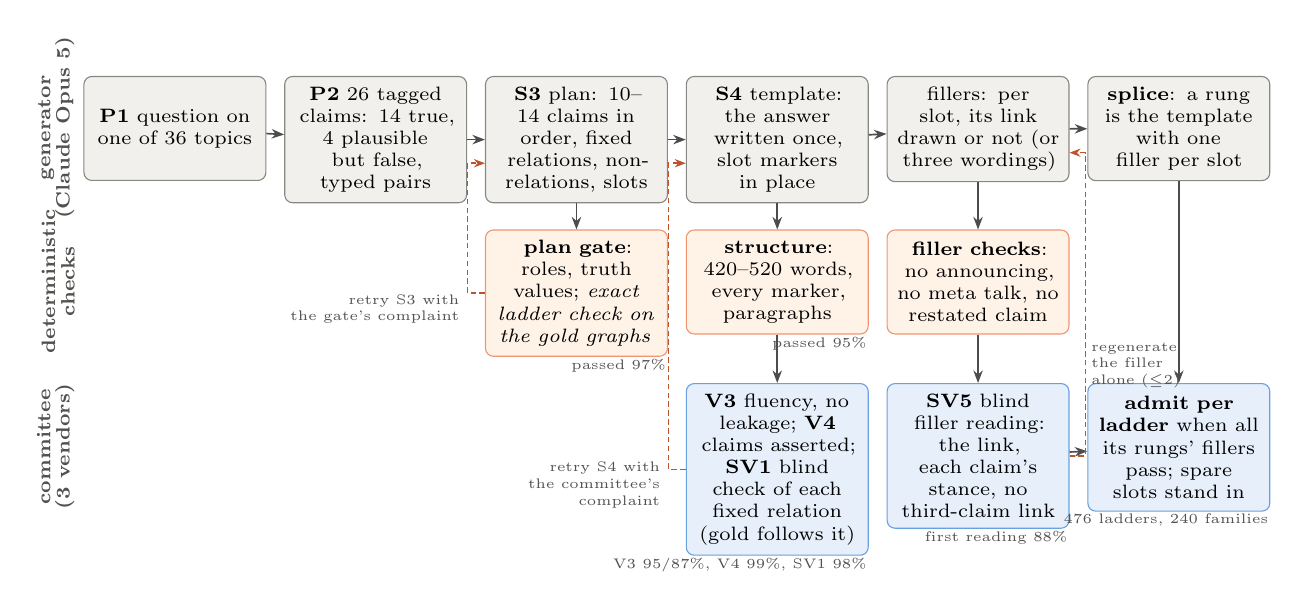
\begin{tikzpicture}[
  font=\scriptsize,
  box/.style={rounded corners=1mm,text width=2.05cm,align=center,inner sep=1.3mm,
              anchor=north},
  gen/.style={box,draw=lbline,fill=lbgen,minimum height=1.32cm},
  det/.style={box,draw=lbconflict!70,fill=lbdet,minimum height=1.32cm},
  com/.style={box,draw=lbsupport!70,fill=lbcom,minimum height=1.62cm},
  flow/.style={-{Stealth[length=1.6mm]},black!70,line width=0.6pt},
  back/.style={-{Stealth[length=1.4mm]},lbconflict!80!black,line width=0.55pt,
               dash pattern=on 2pt off 1.2pt},
  lane/.style={font=\scriptsize\bfseries,text=lbink,rotate=90,anchor=south,align=center},
  rate/.style={font=\tiny,text=lbink,inner sep=0.6pt,anchor=north},
]
\def\gy{0} \def\dy{-1.95} \def\cy{-3.9}
% columns
\foreach \n/\x in {c1/0,c2/2.55,c3/5.1,c4/7.65,c5/10.2,c6/12.75} \coordinate (\n) at (\x,0);
% ---- generator lane ----
\node[gen] (p1) at (c1|-0,\gy) {\textbf{P1} question on one of \lbTopics{} topics};
\node[gen] (p2) at (c2|-0,\gy) {\textbf{P2} 26 tagged claims: 14 true, 4 plausible but false, typed pairs};
\node[gen] (s3) at (c3|-0,\gy) {\textbf{S3} plan: 10--14 claims in order, fixed relations, non-relations, slots};
\node[gen] (s4) at (c4|-0,\gy) {\textbf{S4} template: the answer written once, slot markers in place};
\node[gen] (sf) at (c5|-0,\gy) {fillers: per slot, its link drawn or not (or three wordings)};
\node[gen] (sp) at (c6|-0,\gy) {\textbf{splice}: a rung is the template with one filler per slot};
\foreach \a/\b in {p1/p2,p2/s3,s3/s4,s4/sf,sf/sp} \draw[flow] (\a) -- (\b);
% ---- deterministic lane ----
\node[det] (g3) at (c3|-0,\dy) {\textbf{plan gate}: roles, truth values; \emph{exact ladder check on the gold graphs}};
\node[det] (g4) at (c4|-0,\dy) {\textbf{structure}: 420--520 words, every marker, paragraphs};
\node[det] (gf) at (c5|-0,\dy) {\textbf{filler checks}: no announcing, no meta talk, no restated claim};
\draw[flow] (s3) -- (g3); \draw[flow] (s4) -- (g4); \draw[flow] (sf) -- (gf);
% ---- committee lane ----
\node[com] (tg) at (c4|-0,\cy) {\textbf{V3} fluency, no leakage; \textbf{V4} claims asserted; \textbf{SV1} blind check of each fixed relation (gold follows it)};
\node[com] (sv5) at (c5|-0,\cy) {\textbf{SV5} blind filler reading: the link, each claim's stance, no third-claim link};
\node[com] (adm) at (c6|-0,\cy) {\textbf{admit per ladder} when all its rungs' fillers pass; spare slots stand in};
\draw[flow] (g4) -- (tg); \draw[flow] (gf) -- (sv5); \draw[flow] (sv5) -- (adm);
\draw[flow] (sp) -- (adm);
% ---- retry loops (dashed) ----
\draw[back] (g3.west) -- ++(-0.22,0) |- ([yshift=-3mm]s3.west);
\node[rate,anchor=east,align=right] at ([xshift=-0.3cm,yshift=-0.2cm]g3.west) {retry S3 with\\the gate's complaint};
\draw[back] (tg.west) -- ++(-0.22,0) |- ([yshift=-3mm]s4.west);
\node[rate,anchor=east,align=right] at ([xshift=-0.3cm,yshift=-0.2cm]tg.west) {retry S4 with\\the committee's\\complaint};
\draw[back] (sv5.east) -- ++(0.2,0) |- ([yshift=-3mm]sf.east);
\node[rate,anchor=west,align=left] at ([xshift=0.25cm,yshift=1.15cm]sv5.east) {regenerate\\the filler\\alone ($\le$2)};
% ---- pass rates ----
\node[rate,anchor=north east] at (g3.south east) {passed \lbGateSThreegatePct\%};
\node[rate,anchor=north east] at (g4.south east) {passed \lbGateSFourstructurePct\%};
\node[rate,align=right,anchor=north east] at (tg.south east) {V3 \lbGateVThreescoresPct/\lbGateVThreespansPct\%, V4 \lbGateVFourPct\%, SV1 \lbGateSVOnePct\%};
\node[rate,anchor=north east] at (sv5.south east) {first reading \lbGateSVFivePct\%};
\node[rate,anchor=north east] at (adm.south east) {\lbLadders{} ladders, \lbFamilies{} families};
% ---- lane labels ----
\node[lane] at (-1.15,\gy-0.66) {generator\\[-1pt](Claude Opus~5)};
\node[lane] at (-1.15,\dy-0.66) {deterministic\\[-1pt]checks};
\node[lane] at (-1.15,\cy-0.81) {committee\\[-1pt](3 vendors)};
\end{tikzpicture}
\caption{\textbf{The generation and validation pipeline.} Top: the generator writes a question,
a tagged claim pool, a plan and a template with slot markers, then the fillers of every slot;
every rung is a splice. Middle: deterministic checks, the first of which verifies, before any
prose exists, that each ladder's gold graphs are ordered exactly as declared. Bottom: a committee
of three models from three vendors, never the generator, reads the template and every filler
\emph{blind} to the plan and to the intended link. Dashed: what happens on a failure.
Percentages are pass rates over every evaluation of every attempt (\S\ref{sec:validation}).}
\label{fig:pipeline}
\end{figure*}


One generator (Claude Opus~5) writes every family in five stages (Figure~\ref{fig:pipeline},
top). Every prompt is reproduced verbatim in App.~\ref{app:prompts}.

\paragraph{P1: question.} Each family is assigned a canonical topic, one of \lbTopics{} in
\lbDomains{} domains, and a primary ladder type. The generator writes one open question about the
topic whose answer would naturally contain several kinds of logical relation; the prompt prefers
questions on which competing explanations are adjudicated (incident investigations, diagnostic
reasoning, competing scientific hypotheses), and forbids words such as ``cause'' or ``contrast''
that would prime the relations lexically.

\paragraph{P2: claim pool.} The generator writes 26 atomic claims that an answer to the question
could assert, each a single declarative sentence with no connective, each tagged: 14 factually
correct, 4 plausible but false, and three typed pairs that later relations need (two exhaustive
alternatives, two disjunctive claims, two equivalent claims) plus two holding claims in which an
authority settles a dispute. Nothing in a false claim's wording gives it away. The tags are the
factuality labels of the verdict world: only the 4 incorrect claims are false, and the labels are
set here, before any other stage.

\paragraph{S3: plan.} From the pool, the plan selects 10--14 claims in assertion order (12--14 in
the release), at least two of them false; 6--8 fixed relations among them, each joining claims at
most five positions apart, with a sense and a strength band; 3--5 declared non-relations; and the
slots its ladders need, each joining two consecutive claims and carrying a role. The requirements are
substituted per ladder type (App.~\ref{app:prompts}). Every plan must also use one or two rare
senses, allocated across the corpus so that each of \sense{Alternative}, \sense{Disjunction},
\sense{Restatement}, \sense{Refutation} and \sense{Precedence} appears in \lbRareAlternative{}
plans, rather than demanded of every plan.

\paragraph{The plan gate.} A deterministic gate checks the plan before any prose is written. Each
slot's endpoints must have the truth values its role needs (two true claims for \cp{conflict},
\cp{chain} and \cp{control}; a true claim followed by a false one for \cp{sign}); claims must be
quoted verbatim from the pool and every claim pair used at most once; and, crucially, each
ladder's gold graphs, compiled with the map of Table~\ref{tab:compile}, must be ordered exactly as
declared, at the verdict world, with a step of at least $0.05$ nats in the companion paper's score
between neighbouring rungs, so that no edit is saturated away. A plan that fails is retried with
the gate's complaint; \lbGateSThreegate{} plan evaluations passed.

\paragraph{S4: template and fillers.} The generator then writes the answer once, 420--520 words
in 3--5 paragraphs (4--5 self-contained ones for \cp{order}), with a marker where each slot goes,
together with every filler of every slot. It asserts every non-slot claim exactly once, false ones
in the same confident register as true ones, and realizes every fixed relation with an explicit
connective. The fillers of one slot must be \emph{interchangeable}: the same grammatical frame and
the same reference to the surrounding text, so that swapping fillers changes only the link. An
unlinked filler states its claims plainly without announcing that they are unrelated, and no
filler may talk about ``these claims'' or restate a claim the template already asserts. A deterministic structure check
enforces the length, the markers and the paragraphs. A filler that later fails validation is
regenerated on its own (SF) with the committee's readings as feedback.

\paragraph{Splicing.} Each rung is the template with one filler per marker; spacing is normalized
and nothing else changes. \cp{order} rungs are paragraph permutations of the base splice, each
re-verified by the committee (\S\ref{sec:validation}); a permutation that loses a relation is
replaced by the next candidate. Each rung's gold graph is the plan's fixed relations, as corrected
by the committee, plus the links of its fillers.

%% ============================================================================
\section{Validation}
\label{sec:validation}
%% ============================================================================

A committee of three models from three vendors (GPT-6.1, Gemini~3.1 Pro and Claude Opus~5.5)
validates every family. No committee member is the generator, and every gate is decided by a
majority of three. Figure~\ref{fig:gates} gives the pass rate of every gate.

\paragraph{V3: fluency and leakage.} Each rater scores the template's fluency, formality and
organization on a 1--5 scale and flags hedging and annotation leakage (text that talks about the
claims rather than asserting them). A template passes if a majority scores every criterion at
least 4 and no majority flags a span. V3 reads the \emph{base splice} and also a set of
\emph{coverage splices} that between them contain every filler, so no filler reaches a rung
unread.

\paragraph{V4: claims asserted.} A majority must find every claim asserted, and every false claim
asserted \emph{as written}, so that the template does not silently correct its falsehoods.

\paragraph{SV1: fixed relations, blind.} Each rater is shown the template and a list of claim
pairs, the fixed relations mixed with the declared non-relations, and asked how the text relates
each pair; it does not see the plan. A template stands only if a majority confirms at least
$75\%$ of its fixed relations. Where the majority's reading of a fixed relation or non-relation
departs from the plan, \emph{gold follows the reading}: the relation is dropped, added or
replaced, and the ladder check of \S\ref{sec:generation} is re-run on the corrected graphs. This
happened to \lbGoldCorr{} relations in \lbGoldCorrFamilies{} families (\lbGoldCorrDropped{}
dropped, \lbGoldCorrReplaced{} replaced, \lbGoldCorrAdded{} added; App.~\ref{app:checks}).

\paragraph{SV5: fillers, blind.} Each filler is read in its rung by every rater, who is told
which two claims the slot joins but not which link was intended, and is told to report what
the passage says without using outside knowledge of whether the claims are true. It reports the
link the passage draws between them, each claim's stance (asserted or denied), and any link the filler draws to a
third statement. A filler is admitted if a majority reads exactly the intended link and stances
and no majority reads a third-claim link (Table~\ref{tab:readings}). A rejected filler is
regenerated alone with the readings as feedback, up to twice, and then a spare slot stands in.

\paragraph{Deterministic filler checks.} Before the committee reads a filler, regular expressions
reject fillers that \emph{announce} that their claims are unconnected (``separately'', ``it is
also documented that''), which would mark the unlinked rung for any reader, fillers that talk
\emph{about} the claims (``these two statements cannot both be true''), which read as annotation,
and fillers that restate a claim already in the template (App.~\ref{app:checks}).

\paragraph{Admission.} Admission is per ladder: a ladder is admitted when every one of its rungs'
fillers has passed SV5, and a family is released when at least one ladder survives. Templates
that fail V3, V4 or SV1 are regenerated with the committee's complaint; fillers never cause a
template to be regenerated.

\begin{figure*}[t]
\centering
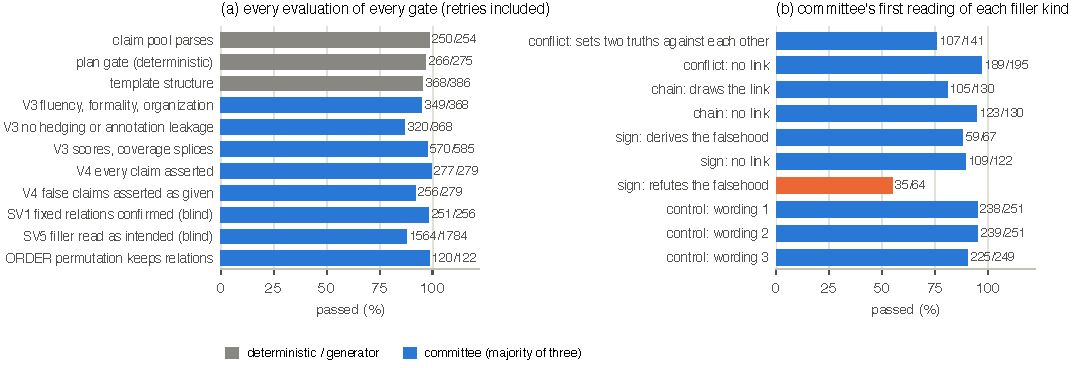
\includegraphics[width=\textwidth]{figures/fig_gates.pdf}
\caption{\textbf{How selective validation is.} (a) Pass rate of every gate over every evaluation
of every attempt (\lbAttempts{} family attempts), retries included. (b) The committee's
\emph{first} reading of each filler kind, before any regeneration: the refuting filler of
\cp{sign} is the hardest to write so that blind readers read a denial and nothing more
(\lbReadSigntfSupport{} on the first try); regeneration repaired almost all of them.}
\label{fig:gates}
\end{figure*}

\begin{table*}[t]
\centering\scriptsize
\rdTable
\caption{\textbf{A filler the committee rejected and the one that replaced it} (family
\rdFamily, \cp{conflict} slot joining $a_{\rdXPos}$: ``\rdX'' and $a_{\rdYPos}$: ``\rdY''). Raters
see the response with the filler in place and the two claims, not the intended link. The first
filler draws the intended incompatibility, but two raters also read a link to a third statement
(the ``since \ldots'' clause), so it is rejected and regenerated; the second is read as intended
by a majority. Readings are the committee's verbatim outputs.}
\label{tab:readings}
\end{table*}

\paragraph{What validation establishes, and what it does not.} The committee confirms relations
by blind pair-by-pair reading, not by the open recovery prompts that relation miners use, so
admission does not select for what a miner recovers. Two dependencies remain. Gold relations are
what the committee read, so a mined graph's agreement with gold is agreement with that reading;
and the committee and the reference miners share vendors, although no model is both. The
factuality labels are the generator's and are not re-verified. Fluency and blind readings are
model judgements; the human study of \S\ref{sec:study} tests them.

%% ============================================================================
\section{The Release}
\label{sec:release}
%% ============================================================================

\begin{table}[t]
\centering\small
\setlength{\tabcolsep}{3pt}
\begin{tabular}{@{}lr@{}}
\toprule
\multicolumn{2}{@{}l}{\emph{Composition}} \\
families, topics, domains & \lbFamilies, \lbTopics, \lbDomains \\
primary ladders, each type & \lbNConflict \\
\cp{control} ladders & \lbNControl \\
responses & \lbItems \\
\midrule
\multicolumn{2}{@{}l}{\emph{Per response}} \\
words & \lbWordsMin--\lbWordsMax{} (median \lbWordsMedian) \\
claims (false) & \lbClaimsMin--\lbClaimsMax{} (\lbFalseMin--\lbFalseMax) \\
relations (with coupling) & \lbRelsMin--\lbRelsMax{} (\lbFactorRelsMin--\lbFactorRelsMax) \\
declared non-relations & \lbNonRelsMin--\lbNonRelsMax \\
\midrule
\multicolumn{2}{@{}l}{\emph{Gold relations, all responses}} \\
total (with a coupling) & \lbRelTotal{} (\lbRelFactor) \\
fixed / from fillers & \lbRelPlan{} / \lbRelSlot \\
strong / moderate / weak & \lbBandStrong{} / \lbBandModerate{} / \lbBandWeak \\
sup.\ / conf., verdict world & \lbRelVerdictSup{} / \lbRelVerdictCon \\
sup.\ / conf., asserted world & \lbRelAssertSup{} / \lbRelAssertCon \\
\midrule
\multicolumn{2}{@{}l}{\emph{Generation}} \\
attempts (admitted first try) & \lbAttempts{} (\lbFirstTry) \\
LLM calls (per ladder) & \lbCalls{} (\lbCallsPerLadder) \\
gateway spend & \$\lbSpend \\
\bottomrule
\end{tabular}
\caption{The released test split.}
\label{tab:release}
\end{table}

\begin{figure*}[t]
\centering
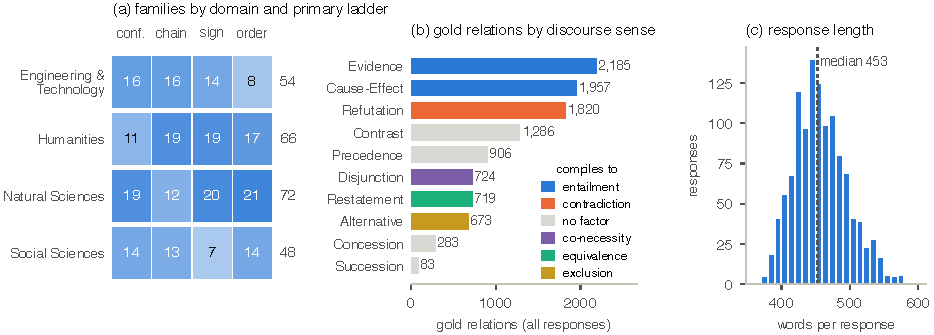
\includegraphics[width=\textwidth]{figures/fig_composition.pdf}
\caption{\textbf{What is in the release.} (a) Families per domain and primary ladder type
(\cp{control} ladders ride on every family). (b) Gold relations by discourse sense over all
responses, coloured by the coupling they compile to; the five rare senses are allocated across
plans. (c) Response length, every rung of every family.}
\label{fig:composition}
\end{figure*}

\paragraph{Composition.} The test split has \lbFamilies{} families, 6--7 on each of
\lbTopics{} topics in \lbDomains{} domains, with every topic carrying all four primary types
(Table~\ref{tab:release}, Figure~\ref{fig:composition}). Family $i$ takes topic $i \bmod 36$ and a
primary type from a shifted rotation, so every type has exactly \lbNConflict{} ladders. A family
has five responses: three on its primary ladder, of which the middle one is also the first rung of
its \cp{control} ladder, and two more on the \cp{control} ladder.

\paragraph{Generation record.} The split took \lbAttempts{} family attempts for \lbFamilies{}
families; \lbFirstTry{} were admitted on the first attempt. Of the \lbAttemptsRejected{} rejected
attempts, \lbRejStageTemplate{} failed at the template (V3 hedging or leakage \lbRejVThreeSpans,
V3 scores \lbRejVThreeScores, V4 false claims corrected \lbRejVFour, structure \lbRejSFour),
\lbRejContentFilter{} were one question that a content filter blocked, and \lbRejSVFive{} had a slot
with no admissible filler. \lbCalls{} LLM calls were made, most of
them committee readings (\lbCallsSVFive{} SV5 and \lbCallsVThree{} V3 calls), about \$\lbSpend{}
at gateway rates. Three events are documented in full in App.~\ref{app:record}. A first attempt
rotated three generators (Claude Opus~5, GPT-6.1, Gemini~3.1 Pro); the prompts, developed on
Claude, so rarely produced admissible templates from the other two that the split was generated
with Claude Opus~5 alone. One family's question was blocked by a provider's content filter and
replaced. Ten families that lost their primary ladder were regenerated from new questions so that
every type has \lbNConflict{} ladders; \lbMissingControl{} \cp{control} ladders failed and are
absent. The gateway caches identical requests, so every run bypasses its cache.

\paragraph{Splits.} A 16-family \emph{development split} (\lbDevLadders{} ladders, \lbDevItems{}
responses), built first and used to develop the prompts, is released separately and is not test
data (App.~\ref{app:dev}).

\paragraph{Format and use.} Each response is one JSON item with its text, claims (with factuality
label and stance), gold relations (with sense, coupling, band, provenance and sign at both
worlds), non-relations and its ladder memberships; a family file lists each ladder's responses in
rung order with its declared order (App.~\ref{app:schema}). A metric is evaluated on \emph{rung
pairs}: each ladder contributes its three pairs, \sThreeNIncPairs{} \emph{Increase} pairs from the
increasing ladders and \sThreeNInvPairs{} \emph{Invariance} pairs from \cp{order} and
\cp{control}. An Increase pair is satisfied by a strict rise, an Invariance pair by equality,
optionally within a tolerance on the metric's own scale; results are reported per ladder type with
family-level bootstrap intervals, since the rungs of a family share a template. The harness
computes all of this from a file of scores per response, and also reports \cp{sign} at both
worlds.

%% ============================================================================
\section{One Family, End to End}
\label{sec:family}
%% ============================================================================

% Figure: a real template with its slot markers, and the slot fillers (examples/*_f009).
\begin{figure*}[t]
\centering
\fbox{\begin{minipage}{0.97\textwidth}\scriptsize\setlength{\parskip}{3pt}
Resolving a dispute of this kind depends less on gathering more evidence than on locating the single observation that only one of the two accounts can accommodate. The standard first move is therefore to audit the platform layer, because a hardware story and a software story predict different distributions of symptoms across machines, releases and code paths. \slotmarker{S1}

\slotmarker{S2} Although correctable errors were logged during that window, ECC memory silently corrects double-bit errors without recording any event, so a sparse log is not by itself a clean bill of health. The machine check exceptions captured across the cluster nevertheless show that a subset of the cluster's memory modules produced uncorrectable errors; the continued failure of hosts whose memory had just been swapped out, by contrast, tells against reading the incident as a pure component defect. At that stage at least one of two conditions had to obtain, and perhaps both held together: uncorrectable errors in the cluster's memory, or an application that accessed shared state without synchronization.

The next step is to interrogate the corrupted output itself and the code that produced it. \slotmarker{S3} It was the unsynchronized sharing of that ring buffer across workers that produced the race condition instrumentation went on to detect. \slotmarker{S4} That sanitizer result confirms the second of the two candidate conditions, namely that the application was reaching shared state without the synchronization its correctness required.

The decisive discrimination comes from the pattern of occurrence rather than from any single log entry. Hardware-induced faults reproduce deterministically on every execution of the same code path; the corrupted responses, by contrast, appeared only on hosts running the new application release. That is, no host running the previous application release produced a corrupted response. The method, in summary, is to treat each account as a prediction about where symptoms should and should not appear, to find the boundary at which one prediction fails, and then to replace inference from telemetry with direct instrumentation of the suspect path.

\end{minipage}}
\par\medskip
{\scriptsize\setlength{\tabcolsep}{2.5pt}
\begin{tabular}{@{}lp{0.86\textwidth}@{}}
\toprule
Filler & Text \\
\midrule
\multicolumn{2}{@{}l}{\slotmarker{S1} conflict slot, $a_{1}$--$a_{2}$} \\
\quad conflict & Platform telemetry recorded machine check exceptions on several hosts in the cluster, a record that cannot be squared with the persistence of the failures on hosts whose memory modules had been freshly replaced. \\
\quad no link & Platform telemetry recorded machine check exceptions on several hosts in the cluster. The failures persisted on hosts whose memory modules had been freshly replaced. \\
\addlinespace
\multicolumn{2}{@{}l}{\slotmarker{S2} conflict slot, $a_{3}$--$a_{4}$} \\
\quad conflict & The ECC subsystem logged correctable single-bit errors on two hosts during the incident window, a signature that cannot be squared with the fact that hardware faults typically cluster on individual machines rather than following a single code path. \\
\quad no link & The ECC subsystem logged correctable single-bit errors on two hosts during the incident window. As a general matter, hardware faults typically cluster on individual machines rather than following a single code path. \\
\addlinespace
\multicolumn{2}{@{}l}{\slotmarker{S3} conflict (spare) slot, $a_{8}$--$a_{9}$} \\
\quad conflict & The corrupted responses carried checksums that did not match their payloads, which rules out the possibility that the suspect code path used a lock-free ring buffer shared between worker threads, as it did. \\
\quad no link & The corrupted responses carried checksums that did not match their payloads. The suspect code path used a lock-free ring buffer shared between worker threads. \\
\addlinespace
\multicolumn{2}{@{}l}{\slotmarker{S4} control slot, $a_{10}$--$a_{11}$} \\
\quad wording 1 & A thread-sanitizer build reported a data race on the ring buffer's write index, and that report led directly to a remediation that added a memory barrier around updates to the shared write index. \\
\quad wording 2 & Because a thread-sanitizer build reported a data race on the ring buffer's write index, the remediation added a memory barrier around updates to the shared write index. \\
\quad wording 3 & The remediation added a memory barrier around updates to the shared write index, a change brought about by a thread-sanitizer build's report of a data race on the ring buffer's write index. \\
\bottomrule
\end{tabular}
}
\caption{\textbf{A template and its fillers} (family f009, the ladder of
Figure~\ref{fig:teaser}). Top: the answer as the generator wrote it once, with four slot markers.
Bottom: each slot's fillers. \cp{conflict} slots S1 and S2 each have an unlinked filler and one
that sets the two claims against each other; S3 is the spare that stands in if S1 or S2 fails
validation (unused here); S4 is the \cp{control} slot, with three wordings of one entailment.
Splicing one filler into every marker yields a rung: the five responses of the family differ only
in these sentences. Full texts of all rungs, the claim list and the gold relations are in
App.~\ref{app:families}.}
\label{fig:template}
\end{figure*}


Figure~\ref{fig:template} shows the template of family f009 and the fillers of its four slots.
Its \cp{conflict} ladder (Figure~\ref{fig:teaser}) splices the refuting fillers into S1 and S2,
then into S1 only, then into neither; its \cp{control} ladder splices the three wordings into S4
while S1 carries its conflict and S2 its unlinked filler, which is the conflict ladder's middle
rung. App.~\ref{app:families} gives this family and one family of every other primary type in
full: the claim list with labels, the template, the fillers, the five responses with their
assignments and gold scores at both worlds, one response in full and its gold relations.

% Figure: one SIGN ladder at the verdict world and at the asserted world (examples/worlds_<fid>).
\begin{figure*}[t]
\centering\small
\setlength{\tabcolsep}{4pt}
\renewcommand{\arraystretch}{1.25}
\begin{tabular}{@{}l >{\raggedright\arraybackslash}p{5.35cm} l cc c cc c@{}}
\toprule
& & & \multicolumn{3}{c}{verdict world} & \multicolumn{3}{c}{asserted world} \\
\cmidrule(lr){4-6}\cmidrule(l){7-9}
Rung & The slot's text & Relation & $x_{\wTruePos}, x_{\wFalsePos}$ & sign & $\LCS$
  & $x_{\wTruePos}, x_{\wFalsePos}$ & sign & $\LCS$ \\
\midrule
$\rho_0$ derives & \csname wTextA\endcsname & \csname wCoupA\endcsname
  & 1, 0 & \csname wSignVTexA\endcsname & \csname wLcsVA\endcsname
  & 1, \csname wXaA\endcsname & \csname wSignATexA\endcsname & \csname wLcsAA\endcsname \\
$\rho_1$ no link & \csname wTextB\endcsname & ---
  & 1, 0 & \csname wSignVTexB\endcsname & \csname wLcsVB\endcsname
  & 1, \csname wXaB\endcsname & \csname wSignATexB\endcsname & \csname wLcsAB\endcsname \\
$\rho_2$ refutes & \csname wTextC\endcsname & \csname wCoupC\endcsname
  & 1, 0 & \csname wSignVTexC\endcsname & \csname wLcsVC\endcsname
  & 1, \csname wXaC\endcsname & \csname wSignATexC\endcsname & \csname wLcsAC\endcsname \\
\bottomrule
\end{tabular}
\caption{\textbf{The same ladder at two committed worlds} (family \wFamily, \cp{sign}). The slot
joins a true claim, $a_{\wTruePos}$: ``\wTrue'', and a false one, $a_{\wFalsePos}$: ``\wFalse''
The \emph{verdict world} sets each claim to its factuality label, $(x_{\wTruePos},
x_{\wFalsePos})=(1,0)$ on every rung. The \emph{asserted world} sets each claim to the response's
stance: both asserted on $\rho_0$ and $\rho_1$, the false claim denied on $\rho_2$. Deriving the
falsehood from the truth violates the entailment at the verdict world (a conflict, $\LCS$ falls)
but upholds it at the asserted world (a support); refuting it is a support at both. So the
declared order $\rho_0<\rho_1<\rho_2$ holds at the verdict world, while the asserted world rates
deriving and refuting the falsehood alike. Both worlds are fixed by the data before any prose is
written (\S\ref{sec:worlds}).}
\label{fig:worlds}
\end{figure*}


Figure~\ref{fig:worlds} follows one \cp{sign} slot through its ladder at both worlds. The slot
joins a true claim to a false one, and its rungs derive the falsehood, draw no link and refute it.
At the verdict world the derivation is a violated entailment and the refutation an upheld
contradiction, so the gold score rises along the ladder; at the asserted world the derivation is
upheld, and the score rates deriving and refuting the falsehood alike. A metric that reads the
response's commitments without the facts cannot tell the two apart, which is what the \cp{sign}
ladder is for.

\begin{figure*}[t]
\centering
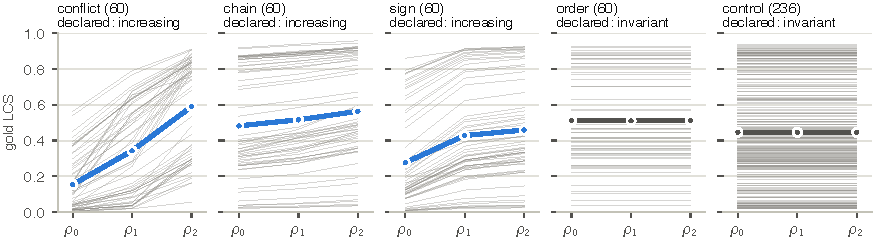
\includegraphics[width=\textwidth]{figures/fig_gold_lcs.pdf}
\caption{\textbf{The gold graphs realize the declared orders.} Gold $\LCS$ \citep{anoncoherence}
per rung for every ladder (gray) and their mean (bold). Every increasing ladder rises strictly at
every step and every invariant ladder is flat, as the plan gate requires; how far a ladder rises
depends on the rest of its graph, which is why \cp{chain} ladders that start near the top of the
scale rise least.}
\label{fig:gold-lcs}
\end{figure*}

Figure~\ref{fig:gold-lcs} shows gold $\LCS$ per rung for every ladder. Every increasing ladder
rises at every step and every invariant ladder is flat, which the plan gate guarantees; the size
of a step depends on the rest of the graph. A \cp{conflict} ladder removes two violated
contradictions and rises most, while a \cp{chain} ladder whose other relations already support its
claims strongly starts near the top of the scale and rises least.

%% ============================================================================
\section{Reference Evaluation}
\label{sec:reference}
%% ============================================================================

The companion paper \citep{anoncoherence} evaluates a coherence score on this split; we summarize
the setup and the results, which also serve as a check of the benchmark.

\paragraph{The score.} The logical coherence score (LCS) reads a Markov random field over the
claims' truth values, with one soft constraint per relation weighted by its strength, at a
committed world $\xs$: $\LCS=\sigma(\operatorname{logit}\PR(\xs)-\operatorname{logit}\pi(\xs))$,
where $\pi$ is the prior and $\PR$ the posterior given the relations. It is the weight of evidence
the relations lend to $\xs$, read on a $[0,1]$ scale, and it is strictly monotone in every
elementary improvement at $\xs$ for any priors and any relation graph. Read at the verdict world,
refuting a falsehood counts as support and deriving one as conflict.

\paragraph{Arms and baselines.} An \emph{arm} fixes where the relation graph comes from: the gold
graphs, or graphs mined from the text by a graph-level miner (GPT-6, and gpt-oss-120b) or a
pairwise miner (gpt-oss-120b and Llama-3.3-70B). Each arm is read at the verdict world (the
paper's score), at the asserted world, and by the mean posterior marginal, a natural but
non-monotone readout. The baselines are ladder-blind controls (claim count, length), DiscoScore and
an entity graph \citep{discoscore}, NLI contradiction and ROSCOE self-consistency over the claims
\citep{roscoe}, and G-Eval and 1--5 rating judges with GPT-6 and gpt-oss-120b, each averaged over
five independent runs \citep{geval}.

\begin{figure*}[t]
\centering
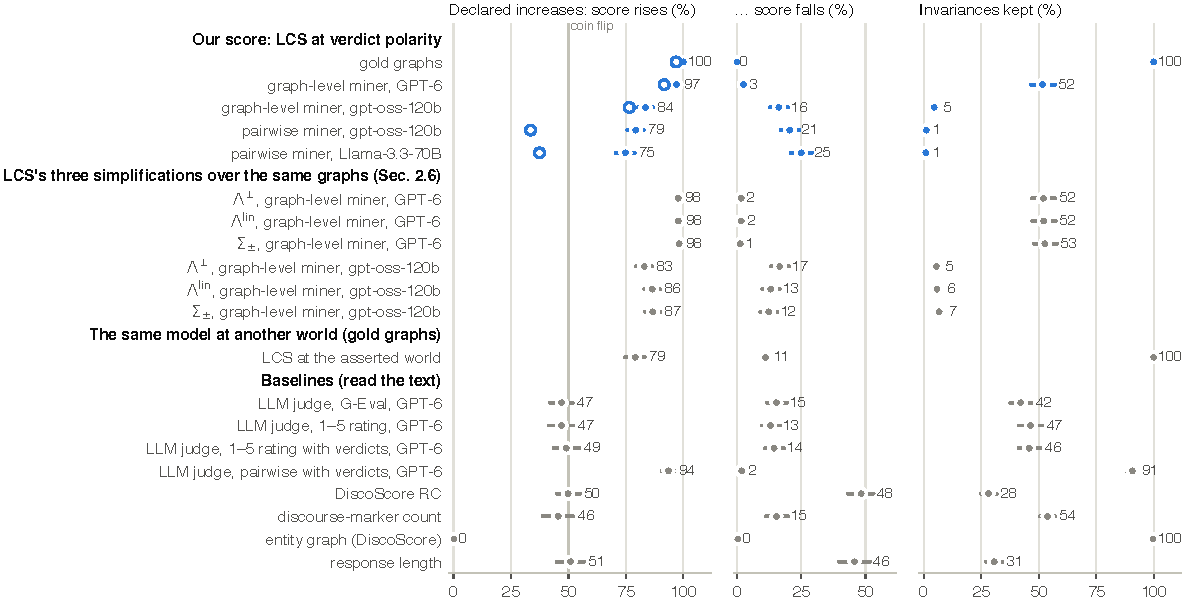
\includegraphics[width=\textwidth]{../coherence/figures/fig_ladders.pdf}
\caption{\textbf{Reference results on the test split} (from the companion paper). For every
score: the share of the \sThreeNIncPairs{} declared increases on which it rises (left) and falls
(middle), and of the \sThreeNInvPairs{} declared invariances it keeps within $0.01$ on its own
scale (right), with 95\% family-bootstrap intervals. Blue: LCS at the verdict world, on gold and
on mined graphs. A score that ignores the edits sits at $0\%$, $0\%$ and $100\%$; a random one at
about $50\%$, $50\%$ and below $100\%$. Hollow markers: invariance kept for a reason other than the
score (saturation, or a score that never changes within a family).}
\label{fig:reference}
\end{figure*}

\paragraph{What the benchmark shows.} Figure~\ref{fig:reference} summarizes the results.
\begin{itemize}[leftmargin=1.2em,itemsep=1pt,topsep=2pt]
\item \textbf{The gold graphs and the score agree.} LCS on gold graphs satisfies
  \sThreeGoldLamInc{} Increase and \sThreeGoldLamInv{} Invariance pairs, as the theory and the
  plan gate predict. This checks the data and the scorer, not new evidence.
\item \textbf{\cp{sign} separates the worlds.} At the asserted world the same score satisfies
  only \sThreeGoldLamASign{} gold \cp{sign} pairs, and the mean marginal \sThreeGoldMMSign: the
  ladder detects whether a metric uses the facts.
\item \textbf{The ladders locate errors in extraction.} With graphs mined by GPT-6, LCS rises on
  \sThreeGraphGptLamIncPct\% of the increases; on every pair whose two mined graphs are ordered as
  declared (\sThreeGraphGptDomForward{} of \sThreeNIncPairs) it rises, so every miss is on a pair
  whose mined graphs the coherence order cannot rank. With pairwise miners it rises on
  \sThreePairOssLamIncPct\% and \sThreePairLlamaLamIncPct\% of the increases, but their
  near-certain weights saturate the score near $0$.
\item \textbf{Surface baselines and judges do not track the edits.} Length passes
  \sThreeBCtlLengthChain{} \cp{chain} pairs because each added link adds words, and fails
  \cp{conflict}. LLM judges rise on \sThreeBGevalGptIncPct\% (G-Eval) and
  \sThreeBDirectGptIncPct\% (rating) of the increases with GPT-6: they read an explicit
  contradiction (\sThreeBGevalGptConflict{} \cp{conflict} pairs for G-Eval) but are close to
  chance on an added inference (\sThreeBGevalGptChain{} rise, \sThreeBGevalGptChainFalls{} fall),
  and keep only \sThreeBGevalGptInvTolUPct\% of the invariances.
\end{itemize}
The benchmark thus discriminates between metrics that respond to the relation an edit changes,
metrics that respond to its surface, and metrics that do not respond at all, and it separates
relation extraction from scoring. Full per-type tables are in App.~\ref{app:reference}.

%% ============================================================================
\section{A Human Validation Study (Planned)}
\label{sec:study}
%% ============================================================================

Every label and every admission decision in LoCoBench is model output. We specify a study that
tests what the construction leaves open; it is pre-registered and has not been run, so its results
are placeholders. The study is scaled to five annotators, the authors, at no more than five hours
each, and all its materials are released (App.~\ref{app:study}).

\paragraph{What the study validates, and why these three.} A declared order is a statement about
gold graphs, which the plan gate checks exactly (\S\ref{sec:declared}). What remains open is
whether the text realizes the graphs, whether people see the orders, and whether the committee
that admitted the data can be trusted.
\begin{description}[leftmargin=1.1em,itemsep=1pt,topsep=2pt,font=\normalfont\bfseries]
\item[1. Filler fidelity.] Rungs differ only in their fillers, and by the monotonicity theorem a
  declared order depends only on the links the fillers draw, whatever the fixed relations are.
  The labels that must be right are therefore the fillers' links: does a filler draw exactly its
  intended link between the slot's claims, with the intended stances, and nothing else?
\item[2. Ordering validity.] Do readers prefer the higher rung of every declared increase, and
  judge the \cp{control} rewordings equal?
\item[3. Committee validity.] Does the committee's blind filler verdict (SV5) agree with people's
  on both sides of the gate? The pipeline kept every filler it rejected, with its readings, so the
  gate can be tested on what it turned away.
\end{description}
Fixed relations are not tested, because they cannot change a declared order; nor are factuality
labels, because the benchmark is defined given the verdicts (annotators are told which claims are
false); nor is \cp{order}, which asks whether paragraph order is part of coherence, a question
about the construct rather than the labels.

\paragraph{Tasks.} \emph{Task 1 (aspects 1 and 3)} shows a filler highlighted in its paragraph,
with the slot's two claims X and Y, and asks what connection the highlighted text draws between
them (eight plain-language options that map onto the committee's labels), whether it asserts,
denies or does not state each claim, and whether it links either claim to any other statement;
this is the committee's SV5 question, put to people. \emph{Task 2 (aspect 2)} shows two complete
responses of one family side by side, with the sentences in which they differ highlighted and the
family's false claims listed as given, and asks which is more logically coherent, or whether they
are about equal. Both are Label Studio projects that each annotator runs locally
(Figure~\ref{fig:study-ui}).

\paragraph{Sample and assignment.} Task 1 has 120 fillers from the test split: 80 that the
committee admitted, 8 for each of the 10 combinations of slot role and filler kind, and 40 that
it rejected, 4 per combination; at most one per family, and none from a Task 2 family. Task 2 has
30 families, 10 each of \cp{conflict}, \cp{chain} and \cp{sign}, round-robin over domains; every
rung pair of their primary and \cp{control} ladders gives 90 Increase and 90 Invariance pairs.
Each item is judged by exactly three annotators, dealt over the ten possible triples so that every
pair of annotators overlaps equally, so each annotator judges 72 fillers and 108 pairs. With a
20-minute practice on the development split and a calibration discussion of the practice items
only, the projected load is 3.5--4 hours per annotator; a pre-registered fallback shrinks Task 1
to 100 fillers if the timed practice projects more than five hours.

\paragraph{Annotators who are the authors.} The annotators know the design, which is the main
threat to validity. Task screens carry no gold, ladder, rung, slot or committee information, and
a build-time check asserts this on every exported task; annotators work alone and do not open the
data. Two features guard against answering from knowledge of the design: Task 1 mixes rejected
with admitted fillers, so ``read as intended'' is not always right, and half of Task 2's pairs
are \cp{control} pairs, whose right answer is ``about equal'', with sides balanced. Each
annotator's screens include six attention checks from the development split; failing two excludes
the annotator. The gold key is committed by its hash in the pre-registration before annotation,
and the analysis refuses a key that does not match. No annotator adjudicates their own
disagreements, and the analysis is scripted.

\begin{table}[t]
\centering\small
\setlength{\tabcolsep}{2.5pt}
\begin{tabular}{@{}p{2.35cm}p{2.8cm}p{1.75cm}@{}}
\toprule
Hypothesis & Test & Result \\
\midrule
H1. Admitted fillers read as intended & exact binomial, rate $>0.80$, $n=80$ & \tbd{} \\
H2. Readers agree with declared increases & sign test, agree vs.\ disagree, $n=90$ (per type, Holm) & \tbd{} \\
H3. \cp{control} pairs read as equal & majority-equal share; side sign test & \tbd{} \\
H4. People agree with the committee & agreement, $\kappa$, reweighted pass and fail rates, $n=120$ & \tbd{} \\
\bottomrule
\end{tabular}
\caption{Pre-registered hypotheses ($\alpha=0.05$). H1 and pooled H2 are confirmatory; per-type
H2, H3 and H4 are reported with 95\% intervals.}
\label{tab:study}
\end{table}

\paragraph{Scoring and analysis.} A person's reading of a filler is scored by the committee's
own rule: the connection must match the intended link (exactly, including direction, for links
that constrain truth; any no-dependence answer for an unlinked filler), every claim the filler
asserts must have the intended stance, and a filler passes when a majority of its readers are
correct and no majority reports a link to another statement. In Task 2 each reader scores a pair
$+1$, $0$ or $-1$ for preferring the declared-higher rung, equal, or the lower one, and the sum
over readers decides agree, tie or disagree. Table~\ref{tab:study} lists the hypotheses. H1
has power $0.90$ at a true rate of $0.92$, and the pooled H2 has power near $1$ if pairs agree
$70\%$ and disagree $15\%$ of the time. Reliability is reported as Krippendorff's $\alpha$
\citep{krippendorff}, nominal for the connection and ordinal for the preference. As secondary
analyses, ladder strengths are fitted with a Bradley--Terry model \citep{bradleyterry}, and every
metric of \S\ref{sec:reference} is rescored against the human majority. Consequences are fixed in
advance: a filler that fails with people is flagged in a release update and every result is
re-run without its family, and a ladder type that fails H2 is reported as not validated by
readers. \tbd{Results.}

%% ============================================================================
\section{Limitations}
\label{sec:limitations}
%% ============================================================================

\textbf{Realism.} The ladders are diagnostic, not a sample of natural responses. Rungs differ in
one or two short sentences, fillers draw their links with explicit markers, and claims are given
rather than extracted, so the benchmark tests whether a metric orders responses whose relations
differ, not how often such differences arise or how well a metric handles implicit links; mined
results on it are best read as upper bounds. \textbf{One generator.} Every family was written by
Claude Opus~5; the prompts were developed on it and did not transfer to two other generators, so
the release reflects one model's style. \textbf{Model-made labels.} The factuality labels are the
generator's and were not verified; gold relations are what the committee read; the human study
that tests both has not been run. \textbf{Coverage.} The relation inventory has ten senses, six
couplings and pairwise relations only, and \cp{sign} covers derivations from a truth to a
falsehood but not the reverse. \textbf{English, expert register.} All families are English
answers in an academic register on \lbTopics{} topics.

\section*{Ethics Statement}

The data are synthetic expert-style answers on academic topics and contain no personal
information. Each response asserts some claims that are false by design; the release labels every
one of them, and the responses should not be used as sources of fact or to train models without
those labels. Generation used commercial models under their terms of use. The planned human study
will be reviewed before data collection and annotators paid at or above the local minimum wage.

\section{Conclusion}

LoCoBench provides what a coherence metric's two requirements need: responses that differ in
argument and in nothing else, with gold graphs and two committed worlds that say what each
response argues and what is true. Its construction checks each declared order exactly before any
prose exists, and validates the prose blind. On it, a monotone score on gold graphs satisfies
every declaration, the \cp{sign} ladder shows whether a metric uses the facts, and errors on mined
graphs are located in extraction; LLM judges miss about half of the declared increases. We release
the data, the pipeline and every prompt, and invite metrics to be evaluated on it.

\bibliography{ref}

\appendix
% Appendix of the LoCoBench dataset paper.

%% ============================================================================
\section{The Pipeline's Prompts, Verbatim}
\label{app:prompts}
%% ============================================================================

Every prompt below is exported from the pipeline's code by
\texttt{scripts/locobench\_export\_prompts.py}, so it is the text that was sent.
\texttt{[\ldots\_PLACEHOLDER]} marks where the pipeline substitutes a value. Prompts in the
function-call idiom (V3, V4, SV1, SV5) follow the committee format of LoReFact \citep{lorefact}:
the model is asked to evaluate a Python call and return JSON.

\subsection{Generation}

\paragraph{P1: topic to question.}
\promptfile{prompts/PROMPT_P1.txt}

\paragraph{P2: question to tagged claim pool.}
\promptfile{prompts/PROMPT_P2.txt}

\paragraph{S3: claims to slot plan.} \texttt{[SENSES\_PLACEHOLDER]} receives the family's one or
two rare senses; \texttt{[SLOTS\_PLACEHOLDER]} receives the slot requirement of its primary ladder
type, given after the prompt.
\promptfile{prompts/PROMPT_S3.txt}

\noindent Slot requirement, \cp{conflict}:
\promptfile{prompts/INSERT_S3_SLOTS_CONFLICT.txt}
\noindent Slot requirement, \cp{chain}:
\promptfile{prompts/INSERT_S3_SLOTS_CHAIN.txt}
\noindent Slot requirement, \cp{sign}:
\promptfile{prompts/INSERT_S3_SLOTS_SIGN.txt}
\noindent Slot requirement, \cp{order}:
\promptfile{prompts/INSERT_S3_SLOTS_ORDER.txt}

\paragraph{S4: plan to template and fillers.} \texttt{[LAYOUT\_PLACEHOLDER]} receives
``Organize the answer into 3-5 paragraphs.'' for \cp{conflict}, \cp{chain} and \cp{sign}, and for
\cp{order}:
\promptfile{prompts/INSERT_S4_LAYOUT_ORDER.txt}
\promptfile{prompts/PROMPT_S4.txt}

\paragraph{SF: regenerating one filler.}
\promptfile{prompts/PROMPT_SF.txt}

\paragraph{Retry notes.} Appended to a prompt whose output failed to parse, or failed a
deterministic check, together with the reason:
\promptfile{prompts/RETRY_PARSE.txt}
\promptfile{prompts/RETRY_SEMANTIC.txt}

\subsection{Committee}

\paragraph{V3: fluency, leakage, hedging, artifacts.}
\promptfile{prompts/PROMPT_V3.txt}

\paragraph{V4: claim coverage.}
\promptfile{prompts/PROMPT_V4.txt}

\paragraph{SV1: blind pair-by-pair relation reading.}
\promptfile{prompts/PROMPT_SV1.txt}

\paragraph{SV5: blind filler reading.}
\promptfile{prompts/PROMPT_SV5.txt}

\subsection{Reference Evaluation}

The prompts of the companion paper's relation miners and LLM judges (\S\ref{sec:reference}).

\paragraph{Graph-level miner.}
\promptfile{prompts/EVAL_GRAPH_MINER.txt}

\paragraph{Pairwise miner, Prompt A (sense and coupling).}
\promptfile{prompts/EVAL_PAIR_A.txt}

\paragraph{Pairwise miner, Prompt B (strength).}
\promptfile{prompts/EVAL_PAIR_B.txt}

\paragraph{G-Eval coherence judge.}
\promptfile{prompts/EVAL_JUDGE_GEVAL.txt}

\paragraph{Direct 1--5 coherence rating.}
\promptfile{prompts/EVAL_JUDGE_DIRECT.txt}

%% ============================================================================
\section{Worked Families}
\label{app:families}
%% ============================================================================

One family of each primary ladder type, extracted from the release by
\texttt{scripts/locobench\_paper\_examples.py}. Each lists the question, the plan's claims with
their labels, the template with its slot markers, every slot's fillers, the five responses with
the filler each carries in the edited slots and its gold $\LCS$ at both worlds, one response in
full with its slot sentences highlighted, and that response's gold relations. The other responses
are the template with the listed fillers spliced in.

\subsection{A \cp{conflict} family (f009)}
% Generated by scripts/locobench_paper_examples.py from f009.
\paragraph{Question.} How do engineers establish whether an intermittent failure in a large distributed system originates in application logic or in the underlying hardware, when the postmortem evidence initially supports two competing accounts? (Computer Science, Engineering \& Technology.)

\paragraph{Claims.} The plan's claims in assertion order, with their factuality labels; claims joined by a ladder's slots are boxed.

\begin{center}\scriptsize
\setlength{\tabcolsep}{2.5pt}
\begin{tabular}{@{}rp{0.76\linewidth}l@{}}
\toprule
& Claim & Label \\
\midrule
\slotclaim{$a_{1}$} & Platform telemetry recorded machine check exceptions on several hosts in the cluster. & true \\
\slotclaim{$a_{2}$} & The failures persisted on hosts whose memory modules had been freshly replaced. & true \\
\slotclaim{$a_{3}$} & The ECC subsystem logged correctable single-bit errors on two hosts during the incident window. & true \\
\slotclaim{$a_{4}$} & Hardware faults typically cluster on individual machines rather than following a single code path. & true \\
$a_{5}$ & ECC memory silently corrects double-bit errors without recording any event. & \textbf{false} \\
$a_{6}$ & A subset of the cluster's memory modules produced uncorrectable errors. & true \\
$a_{7}$ & The application accessed shared state without synchronization. & true \\
$a_{8}$ & The corrupted responses carried checksums that did not match their payloads. & true \\
$a_{9}$ & The suspect code path used a lock-free ring buffer shared between worker threads. & true \\
\slotclaim{$a_{10}$} & A thread-sanitizer build reported a data race on the ring buffer's write index. & true \\
\slotclaim{$a_{11}$} & The remediation added a memory barrier around updates to the shared write index. & true \\
$a_{12}$ & Hardware-induced faults reproduce deterministically on every execution of the same code path. & \textbf{false} \\
$a_{13}$ & Corrupted responses appeared only on hosts running the new application release. & true \\
$a_{14}$ & No host running the previous application release produced a corrupted response. & true \\
\bottomrule
\end{tabular}
\end{center}

\paragraph{Template.} The answer as written once, with its slot markers.

\begin{quote}\small
Resolving a dispute of this kind depends less on gathering more evidence than on locating the single observation that only one of the two accounts can accommodate. The standard first move is therefore to audit the platform layer, because a hardware story and a software story predict different distributions of symptoms across machines, releases and code paths. \slotmarker{S1}

\slotmarker{S2} Although correctable errors were logged during that window, ECC memory silently corrects double-bit errors without recording any event, so a sparse log is not by itself a clean bill of health. The machine check exceptions captured across the cluster nevertheless show that a subset of the cluster's memory modules produced uncorrectable errors; the continued failure of hosts whose memory had just been swapped out, by contrast, tells against reading the incident as a pure component defect. At that stage at least one of two conditions had to obtain, and perhaps both held together: uncorrectable errors in the cluster's memory, or an application that accessed shared state without synchronization.

The next step is to interrogate the corrupted output itself and the code that produced it. \slotmarker{S3} It was the unsynchronized sharing of that ring buffer across workers that produced the race condition instrumentation went on to detect. \slotmarker{S4} That sanitizer result confirms the second of the two candidate conditions, namely that the application was reaching shared state without the synchronization its correctness required.

The decisive discrimination comes from the pattern of occurrence rather than from any single log entry. Hardware-induced faults reproduce deterministically on every execution of the same code path; the corrupted responses, by contrast, appeared only on hosts running the new application release. That is, no host running the previous application release produced a corrupted response. The method, in summary, is to treat each account as a prediction about where symptoms should and should not appear, to find the boundary at which one prediction fails, and then to replace inference from telemetry with direct instrumentation of the suspect path.
\end{quote}

\paragraph{Fillers.} Each slot's fillers, as admitted by the committee.

\begin{center}\scriptsize
\setlength{\tabcolsep}{2.5pt}
\begin{tabular}{@{}lp{0.80\linewidth}@{}}
\toprule
Filler & Text \\
\midrule
\multicolumn{2}{@{}l}{\slotmarker{S1} conflict slot, $a_{1}$--$a_{2}$} \\
\quad conflict & Platform telemetry recorded machine check exceptions on several hosts in the cluster, a record that cannot be squared with the persistence of the failures on hosts whose memory modules had been freshly replaced. \\
\quad no link & Platform telemetry recorded machine check exceptions on several hosts in the cluster. The failures persisted on hosts whose memory modules had been freshly replaced. \\
\addlinespace
\multicolumn{2}{@{}l}{\slotmarker{S2} conflict slot, $a_{3}$--$a_{4}$} \\
\quad conflict & The ECC subsystem logged correctable single-bit errors on two hosts during the incident window, a signature that cannot be squared with the fact that hardware faults typically cluster on individual machines rather than following a single code path. \\
\quad no link & The ECC subsystem logged correctable single-bit errors on two hosts during the incident window. As a general matter, hardware faults typically cluster on individual machines rather than following a single code path. \\
\addlinespace
\multicolumn{2}{@{}l}{\slotmarker{S3} conflict (spare) slot, $a_{8}$--$a_{9}$} \\
\quad conflict & The corrupted responses carried checksums that did not match their payloads, which rules out the possibility that the suspect code path used a lock-free ring buffer shared between worker threads, as it did. \\
\quad no link & The corrupted responses carried checksums that did not match their payloads. The suspect code path used a lock-free ring buffer shared between worker threads. \\
\addlinespace
\multicolumn{2}{@{}l}{\slotmarker{S4} control slot, $a_{10}$--$a_{11}$} \\
\quad wording 1 & A thread-sanitizer build reported a data race on the ring buffer's write index, and that report led directly to a remediation that added a memory barrier around updates to the shared write index. \\
\quad wording 2 & Because a thread-sanitizer build reported a data race on the ring buffer's write index, the remediation added a memory barrier around updates to the shared write index. \\
\quad wording 3 & The remediation added a memory barrier around updates to the shared write index, a change brought about by a thread-sanitizer build's report of a data race on the ring buffer's write index. \\
\bottomrule
\end{tabular}
\end{center}

\paragraph{Rungs.} The five responses of the family, which filler each carries in the edited slots, and gold $\LCS$ at the verdict and the asserted world.

\begin{center}\scriptsize
\setlength{\tabcolsep}{2.5pt}
\begin{tabular}{@{}l>{\raggedright\arraybackslash}p{0.27\linewidth}>{\raggedright\arraybackslash}p{0.30\linewidth}cc@{}}
\toprule
& Ladder, rung & Fillers & \multicolumn{2}{c}{$\LCS$ at world} \\
& & & verdict & asserted \\
\midrule
t0 & conflict $\rho_0$ & S1: conflict, S2: conflict & 0.151 & 0.151 \\
t1 & conflict $\rho_1$, control $\rho_0$ & S1: conflict, S2: no link & 0.343 & 0.343 \\
t2 & conflict $\rho_2$ & S1: no link, S2: no link & 0.849 & 0.849 \\
t3 & control $\rho_1$ & S4: wording 2 & 0.343 & 0.343 \\
t4 & control $\rho_2$ & S4: wording 3 & 0.343 & 0.343 \\
\bottomrule
\end{tabular}
\end{center}

\paragraph{Response t1 in full} (conflict $\rho_1$; edited slots highlighted, 447 words).

\begin{quote}\small
Resolving a dispute of this kind depends less on gathering more evidence than on locating the single observation that only one of the two accounts can accommodate. The standard first move is therefore to audit the platform layer, because a hardware story and a software story predict different distributions of symptoms across machines, releases and code paths. \slotfill{S1}{Platform telemetry recorded machine check exceptions on several hosts in the cluster, a record that cannot be squared with the persistence of the failures on hosts whose memory modules had been freshly replaced.}

\slotfill{S2}{The ECC subsystem logged correctable single-bit errors on two hosts during the incident window. As a general matter, hardware faults typically cluster on individual machines rather than following a single code path.} Although correctable errors were logged during that window, ECC memory silently corrects double-bit errors without recording any event, so a sparse log is not by itself a clean bill of health. The machine check exceptions captured across the cluster nevertheless show that a subset of the cluster's memory modules produced uncorrectable errors; the continued failure of hosts whose memory had just been swapped out, by contrast, tells against reading the incident as a pure component defect. At that stage at least one of two conditions had to obtain, and perhaps both held together: uncorrectable errors in the cluster's memory, or an application that accessed shared state without synchronization.

The next step is to interrogate the corrupted output itself and the code that produced it. The corrupted responses carried checksums that did not match their payloads. The suspect code path used a lock-free ring buffer shared between worker threads. It was the unsynchronized sharing of that ring buffer across workers that produced the race condition instrumentation went on to detect. \slotfill{S4}{A thread-sanitizer build reported a data race on the ring buffer's write index, and that report led directly to a remediation that added a memory barrier around updates to the shared write index.} That sanitizer result confirms the second of the two candidate conditions, namely that the application was reaching shared state without the synchronization its correctness required.

The decisive discrimination comes from the pattern of occurrence rather than from any single log entry. Hardware-induced faults reproduce deterministically on every execution of the same code path; the corrupted responses, by contrast, appeared only on hosts running the new application release. That is, no host running the previous application release produced a corrupted response. The method, in summary, is to treat each account as a prediction about where symptoms should and should not appear, to find the boundary at which one prediction fails, and then to replace inference from telemetry with direct instrumentation of the suspect path.
\end{quote}

\paragraph{Gold relations of response t1.} Sense, compiled coupling, strength band, and the relation's sign at the verdict (v.) and asserted (a.) world ($+$ support, $-$ conflict, $\cdot$ no factor); a slot id marks a relation drawn by a filler.

\begin{center}\scriptsize
\setlength{\tabcolsep}{2.2pt}
\begin{tabular}{@{}lllllcc@{}}
\toprule
Pair & & Sense & Coupling & Band & v. & a. \\
\midrule
$a_{1}\to a_{2}$ & S1 & Refutation & contradiction & strong & $-$ & $-$ \\
$a_{1}\to a_{6}$ &  & Evidence & entailment & moderate & $+$ & $+$ \\
$a_{2}\to a_{6}$ &  & Contrast & none & moderate & $\cdot$ & $\cdot$ \\
$a_{3}\to a_{5}$ &  & Concession & none & moderate & $\cdot$ & $\cdot$ \\
$a_{6}\to a_{7}$ &  & Disjunction & co-necessity & strong & $+$ & $+$ \\
$a_{9}\to a_{10}$ &  & Cause-Effect & entailment & moderate & $+$ & $+$ \\
$a_{10}\to a_{7}$ &  & Evidence & entailment & strong & $+$ & $+$ \\
$a_{10}\to a_{11}$ & S4 & Cause-Effect & entailment & strong & $+$ & $+$ \\
$a_{12}\to a_{13}$ &  & Contrast & none & moderate & $\cdot$ & $\cdot$ \\
$a_{13}\to a_{14}$ &  & Restatement & equivalence & strong & $+$ & $+$ \\
\bottomrule
\end{tabular}
\end{center}


\subsection{A \cp{chain} family (f224)}
% Generated by scripts/locobench_paper_examples.py from f224.
\paragraph{Question.} How do economists adjudicate between the claim that the 1970s stagflation originated in oil supply shocks and the claim that it originated in monetary policy errors, and what evidence settled the dispute? (Economics, Social Sciences.)

\paragraph{Claims.} The plan's claims in assertion order, with their factuality labels; claims joined by a ladder's slots are boxed.

\begin{center}\scriptsize
\setlength{\tabcolsep}{2.5pt}
\begin{tabular}{@{}rp{0.76\linewidth}l@{}}
\toprule
& Claim & Label \\
\midrule
\slotclaim{$a_{1}$} & OPEC imposed an oil embargo on the United States in October 1973. & true \\
\slotclaim{$a_{2}$} & The price of crude oil roughly quadrupled between 1973 and early 1974. & true \\
\slotclaim{$a_{3}$} & Hamilton documented a statistical relationship between oil price increases and postwar US recessions. & true \\
$a_{4}$ & Oil supply shocks account for the entire rise in US inflation during the 1970s. & \textbf{false} \\
$a_{5}$ & US consumer price inflation exceeded 5 percent before the October 1973 oil embargo. & true \\
$a_{6}$ & US consumer price inflation remained below 5 percent until the October 1973 oil embargo. & true \\
$a_{7}$ & OPEC production cuts sharply raised the real price of crude oil in 1973 and 1974. & true \\
$a_{8}$ & US money growth accelerated in the years preceding 1973. & true \\
$a_{9}$ & Japan experienced lower consumer price inflation than the United States in 1974. & \textbf{false} \\
$a_{10}$ & The Federal Reserve's policy interest rate stood below the rate of inflation for much of the 1970s. & true \\
$a_{11}$ & Real policy interest rates in the United States were negative during much of the 1970s. & true \\
$a_{12}$ & Clarida, Gali and Gertler estimated that the pre-1979 Federal Reserve policy rule violated the Taylor principle. & true \\
\slotclaim{$a_{13}$} & Paul Volcker became chairman of the Federal Reserve in August 1979. & true \\
\slotclaim{$a_{14}$} & The Volcker tightening pushed the federal funds rate above 19 percent in 1981. & true \\
\bottomrule
\end{tabular}
\end{center}

\paragraph{Template.} The answer as written once, with its slot markers.

\begin{quote}\small
Adjudicating between the supply-shock and the monetary-policy accounts of the 1970s turns on timing, on cross-country comparison, and on the estimated behaviour of the central bank's reaction function. \slotmarker{S1} \slotmarker{S2} That recession regularity indicates that oil supply shocks account for the entire rise in US inflation during the 1970s.

The chronology, however, disciplines any such attribution. Only two descriptions of the pre-embargo record are available, and exactly one of them can be correct: either US consumer price inflation exceeded 5 percent before the October 1973 oil embargo, or it remained below 5 percent until that embargo. The published price indices place the decade in the first case, and inflation already above 5 percent in advance of the embargo cannot be squared with the view that oil supply shocks produced the whole of the decade's inflation. What can be affirmed is that at least one of two impulses was in operation, and perhaps both were: OPEC production cuts sharply raised the real price of crude oil in 1973 and 1974, and US money growth accelerated in the years preceding 1973.

The monetary side of the ledger rests on further evidence. Japan experienced lower consumer price inflation than the United States in 1974. The Federal Reserve's policy interest rate stood below the rate of inflation for much of the 1970s; in other words, real policy interest rates in the United States were negative during much of the decade, and the Japanese comparison for 1974 is precisely the sort of international evidence that shows those American real rates to have been negative. That sustained shortfall of real rates below zero is in turn evidence for the estimate of Clarida, Gali and Gertler that the pre-1979 Federal Reserve policy rule violated the Taylor principle: a central bank that raises its nominal rate by less than one-for-one with inflation will let real rates fall as prices accelerate.

The dispute was settled less by any single regression than by an institutional experiment at the close of the decade. \slotmarker{S3} The lesson drawn from that episode is that a determined central bank can end an inflation whose proximate trigger lay in commodity markets, and the weight of professional judgment shifted accordingly toward the monetary account.
\end{quote}

\paragraph{Fillers.} Each slot's fillers, as admitted by the committee.

\begin{center}\scriptsize
\setlength{\tabcolsep}{2.5pt}
\begin{tabular}{@{}lp{0.80\linewidth}@{}}
\toprule
Filler & Text \\
\midrule
\multicolumn{2}{@{}l}{\slotmarker{S1} chain link slot, $a_{1}$--$a_{2}$} \\
\quad support & OPEC imposed an oil embargo on the United States in October 1973, and that embargo caused the price of crude oil to roughly quadruple between 1973 and early 1974. \\
\quad no link & OPEC imposed an oil embargo on the United States in October 1973. The price of crude oil, which can be traced through posted contract terms, roughly quadrupled between 1973 and early 1974. \\
\addlinespace
\multicolumn{2}{@{}l}{\slotmarker{S2} chain link slot, $a_{2}$--$a_{3}$} \\
\quad support & A quadrupling of that magnitude confirms the statistical relationship Hamilton documented between oil price increases and postwar US recessions. \\
\quad no link & Hamilton, working through the postwar US record, documented a statistical relationship between oil price increases and recessions. \\
\addlinespace
\multicolumn{2}{@{}l}{\slotmarker{S3} control slot, $a_{13}$--$a_{14}$} \\
\quad wording 1 & Paul Volcker became chairman of the Federal Reserve in August 1979, and his arrival led to a tightening that pushed the federal funds rate above 19 percent in 1981. \\
\quad wording 2 & The federal funds rate was driven above 19 percent in 1981 by the tightening that resulted from Paul Volcker's accession to the chairmanship of the Federal Reserve in August 1979. \\
\quad wording 3 & Because Paul Volcker took charge of the Federal Reserve as chairman in August 1979, a tightening followed that carried the federal funds rate past 19 percent in 1981. \\
\bottomrule
\end{tabular}
\end{center}

\paragraph{Rungs.} The five responses of the family, which filler each carries in the edited slots, and gold $\LCS$ at the verdict and the asserted world.

\begin{center}\scriptsize
\setlength{\tabcolsep}{2.5pt}
\begin{tabular}{@{}l>{\raggedright\arraybackslash}p{0.27\linewidth}>{\raggedright\arraybackslash}p{0.30\linewidth}cc@{}}
\toprule
& Ladder, rung & Fillers & \multicolumn{2}{c}{$\LCS$ at world} \\
& & & verdict & asserted \\
\midrule
t0 & chain $\rho_0$ & S1: no link, S2: no link & 0.337 & 0.067 \\
t1 & chain $\rho_1$, control $\rho_0$ & S1: support, S2: no link & 0.398 & 0.086 \\
t2 & chain $\rho_2$ & S1: support, S2: support & 0.478 & 0.115 \\
t3 & control $\rho_1$ & S3: wording 2 & 0.398 & 0.086 \\
t4 & control $\rho_2$ & S3: wording 3 & 0.398 & 0.086 \\
\bottomrule
\end{tabular}
\end{center}

\paragraph{Response t1 in full} (chain $\rho_1$; edited slots highlighted, 440 words).

\begin{quote}\small
Adjudicating between the supply-shock and the monetary-policy accounts of the 1970s turns on timing, on cross-country comparison, and on the estimated behaviour of the central bank's reaction function. \slotfill{S1}{OPEC imposed an oil embargo on the United States in October 1973, and that embargo caused the price of crude oil to roughly quadruple between 1973 and early 1974.} \slotfill{S2}{Hamilton, working through the postwar US record, documented a statistical relationship between oil price increases and recessions.} That recession regularity indicates that oil supply shocks account for the entire rise in US inflation during the 1970s.

The chronology, however, disciplines any such attribution. Only two descriptions of the pre-embargo record are available, and exactly one of them can be correct: either US consumer price inflation exceeded 5 percent before the October 1973 oil embargo, or it remained below 5 percent until that embargo. The published price indices place the decade in the first case, and inflation already above 5 percent in advance of the embargo cannot be squared with the view that oil supply shocks produced the whole of the decade's inflation. What can be affirmed is that at least one of two impulses was in operation, and perhaps both were: OPEC production cuts sharply raised the real price of crude oil in 1973 and 1974, and US money growth accelerated in the years preceding 1973.

The monetary side of the ledger rests on further evidence. Japan experienced lower consumer price inflation than the United States in 1974. The Federal Reserve's policy interest rate stood below the rate of inflation for much of the 1970s; in other words, real policy interest rates in the United States were negative during much of the decade, and the Japanese comparison for 1974 is precisely the sort of international evidence that shows those American real rates to have been negative. That sustained shortfall of real rates below zero is in turn evidence for the estimate of Clarida, Gali and Gertler that the pre-1979 Federal Reserve policy rule violated the Taylor principle: a central bank that raises its nominal rate by less than one-for-one with inflation will let real rates fall as prices accelerate.

The dispute was settled less by any single regression than by an institutional experiment at the close of the decade. \slotfill{S3}{Paul Volcker became chairman of the Federal Reserve in August 1979, and his arrival led to a tightening that pushed the federal funds rate above 19 percent in 1981.} The lesson drawn from that episode is that a determined central bank can end an inflation whose proximate trigger lay in commodity markets, and the weight of professional judgment shifted accordingly toward the monetary account.
\end{quote}

\paragraph{Gold relations of response t1.} Sense, compiled coupling, strength band, and the relation's sign at the verdict (v.) and asserted (a.) world ($+$ support, $-$ conflict, $\cdot$ no factor); a slot id marks a relation drawn by a filler.

\begin{center}\scriptsize
\setlength{\tabcolsep}{2.2pt}
\begin{tabular}{@{}lllllcc@{}}
\toprule
Pair & & Sense & Coupling & Band & v. & a. \\
\midrule
$a_{1}\to a_{2}$ & S1 & Cause-Effect & entailment & strong & $+$ & $+$ \\
$a_{3}\to a_{4}$ &  & Evidence & entailment & weak & $-$ & $+$ \\
$a_{5}\to a_{4}$ &  & Refutation & contradiction & strong & $+$ & $-$ \\
$a_{5}\to a_{6}$ &  & Alternative & exclusive & strong & $-$ & $-$ \\
$a_{7}\to a_{8}$ &  & Disjunction & co-necessity & strong & $+$ & $+$ \\
$a_{9}\to a_{11}$ &  & Evidence & entailment & weak & $+$ & $+$ \\
$a_{10}\to a_{11}$ &  & Restatement & equivalence & strong & $+$ & $+$ \\
$a_{11}\to a_{12}$ &  & Evidence & entailment & moderate & $+$ & $+$ \\
$a_{13}\to a_{14}$ & S3 & Cause-Effect & entailment & strong & $+$ & $+$ \\
\bottomrule
\end{tabular}
\end{center}


\subsection{A \cp{sign} family (f003)}
% Generated by scripts/locobench_paper_examples.py from f003.
\paragraph{Question.} How did astronomers establish whether the ``Great Debate'' nebulae lay within the Milky Way or formed separate galaxies, and what evidence ultimately settled the dispute? (Astronomy, Natural Sciences.)

\paragraph{Claims.} The plan's claims in assertion order, with their factuality labels; claims joined by a ladder's slots are boxed.

\begin{center}\scriptsize
\setlength{\tabcolsep}{2.5pt}
\begin{tabular}{@{}rp{0.76\linewidth}l@{}}
\toprule
& Claim & Label \\
\midrule
$a_{1}$ & The Great Debate was held on 26 April 1920 at the Smithsonian Museum of Natural History in Washington, D.C. & true \\
$a_{2}$ & Harlow Shapley argued that the spiral nebulae were gaseous clouds lying inside a single large Milky Way system. & true \\
$a_{3}$ & Heber Curtis argued that the spiral nebulae were distant stellar systems comparable in size to the Milky Way. & true \\
\slotclaim{$a_{4}$} & Curtis cited novae observed in spiral nebulae as evidence that those nebulae lay at great distances. & true \\
\slotclaim{$a_{5}$} & Curtis's analysis of novae in spiral nebulae placed M31 about 10,000 light years from the Sun. & \textbf{false} \\
$a_{6}$ & S Andromedae, which appeared in 1885, was a supernova far more luminous than an ordinary nova. & true \\
$a_{7}$ & Shapley relied on Adriaan van Maanen's reported measurements of internal rotation in spiral nebulae. & true \\
$a_{8}$ & Van Maanen's measurements of rotation in spiral nebulae were confirmed by later photographic plate comparisons. & \textbf{false} \\
$a_{9}$ & A later reexamination of van Maanen's plates concluded that the reported rotations of spiral nebulae were measurement artifacts. & true \\
$a_{10}$ & Henrietta Leavitt established the period-luminosity relation from Cepheid variables in the Magellanic Clouds. & true \\
\slotclaim{$a_{11}$} & Edwin Hubble identified Cepheid variable stars in M31 using the 100-inch Hooker telescope at Mount Wilson. & true \\
\slotclaim{$a_{12}$} & Hubble derived a distance to M31 of roughly 900,000 light years. & true \\
$a_{13}$ & M31 lies outside the boundaries of the Milky Way system. & true \\
$a_{14}$ & M31 lies within the boundaries of the Milky Way system. & true \\
\bottomrule
\end{tabular}
\end{center}

\paragraph{Template.} The answer as written once, with its slot markers.

\begin{quote}\small
The status of the spiral nebulae was first contested in open argument and only afterwards resolved by measurement. The Great Debate was held on 26 April 1920 at the Smithsonian Museum of Natural History in Washington, D.C. Harlow Shapley argued that the spiral nebulae were gaseous clouds lying inside a single large Milky Way system, whereas Heber Curtis argued that the spiral nebulae were distant stellar systems comparable in size to the Milky Way. The issue therefore turned on distance, and distance could be extracted only from objects of known intrinsic brightness.

\slotmarker{S1} By contrast, S Andromedae, which appeared in 1885, was a supernova far more luminous than an ordinary nova. The two classes of outburst were not yet separated in the photometry then available, so the eruptions recorded in the spirals could not yet be made to yield a secure scale.

Shapley's case for a single, all-encompassing system rested on evidence of a quite different kind, namely apparent motion within the spirals themselves, since a nebula visibly turning on a human timescale would have to be small and close at hand. \slotmarker{S2} A later reexamination of van Maanen's plates concluded that the reported rotations of spiral nebulae were measurement artifacts, and that verdict cannot be squared with any claim that subsequent comparisons of photographic plates had confirmed those rotations.

Resolution came from a calibrated distance indicator rather than from debate. Earlier, Henrietta Leavitt established the period-luminosity relation from Cepheid variables in the Magellanic Clouds; the search for such stars in the spirals came only afterwards. \slotmarker{S3} A figure of that magnitude demonstrates that M31 lies outside the boundaries of the Milky Way system. The two placements exclude one another: either M31 lies beyond the Galaxy's confines, or M31 lies within the boundaries of the Milky Way system, and exactly one of these must hold. On the Cepheid evidence, the spirals are stellar systems in their own right.
\end{quote}

\paragraph{Fillers.} Each slot's fillers, as admitted by the committee.

\begin{center}\scriptsize
\setlength{\tabcolsep}{2.5pt}
\begin{tabular}{@{}lp{0.80\linewidth}@{}}
\toprule
Filler & Text \\
\midrule
\multicolumn{2}{@{}l}{\slotmarker{S1} sign slot, $a_{4}$--$a_{5}$} \\
\quad conflict & Curtis cited novae observed in spiral nebulae as evidence that those nebulae lay at great distances; that evidence indicates a remove for M31 of about 10,000 light years from the Sun, the figure his analysis of those novae yielded. \\
\quad no link & Curtis cited novae observed in spiral nebulae as evidence that those nebulae lay at great distances. His analysis of novae in spiral nebulae placed M31 about 10,000 light years from the Sun. \\
\quad support & Curtis cited novae observed in spiral nebulae as evidence that those nebulae lay at great distances, and that evidence rules out the claim, sometimes attached to his analysis of novae in spiral nebulae, that it placed M31 about 10,000 light years from the Sun. \\
\addlinespace
\multicolumn{2}{@{}l}{\slotmarker{S2} sign (spare) slot, $a_{7}$--$a_{8}$} \\
\quad conflict & Shapley relied on Adriaan van Maanen's reported measurements of internal rotation in spiral nebulae, and that reliance shows that the rotations van Maanen reported were confirmed by later comparisons of photographic plates. \\
\quad no link & Shapley relied on Adriaan van Maanen's reported measurements of internal rotation in spiral nebulae. The rotations van Maanen reported were confirmed by later comparisons of photographic plates. \\
\quad support & Shapley relied on Adriaan van Maanen's reported measurements of internal rotation in spiral nebulae, and because nothing beyond those original reports of rotation stood behind the figures, the rotations cannot have been confirmed by later comparisons of photographic plates. \\
\addlinespace
\multicolumn{2}{@{}l}{\slotmarker{S3} control slot, $a_{11}$--$a_{12}$} \\
\quad wording 1 & Edwin Hubble identified Cepheid variable stars in M31 using the 100-inch Hooker telescope at Mount Wilson, and that identification led him to a distance for the nebula of roughly 900,000 light years. \\
\quad wording 2 & Because Edwin Hubble was able to pick out Cepheid variable stars in M31 with the 100-inch Hooker telescope at Mount Wilson, a distance of roughly 900,000 light years followed for that nebula. \\
\quad wording 3 & A distance to M31 of roughly 900,000 light years was the direct result of Edwin Hubble's detection of Cepheid variable stars in that nebula with the 100-inch Hooker telescope at Mount Wilson. \\
\bottomrule
\end{tabular}
\end{center}

\paragraph{Rungs.} The five responses of the family, which filler each carries in the edited slots, and gold $\LCS$ at the verdict and the asserted world.

\begin{center}\scriptsize
\setlength{\tabcolsep}{2.5pt}
\begin{tabular}{@{}l>{\raggedright\arraybackslash}p{0.27\linewidth}>{\raggedright\arraybackslash}p{0.30\linewidth}cc@{}}
\toprule
& Ladder, rung & Fillers & \multicolumn{2}{c}{$\LCS$ at world} \\
& & & verdict & asserted \\
\midrule
t0 & sign $\rho_0$ & S1: conflict & 0.123 & 0.036 \\
t1 & sign $\rho_1$, control $\rho_0$ & S1: no link & 0.292 & 0.030 \\
t2 & sign $\rho_2$ & S1: support & 0.334 & 0.036 \\
t3 & control $\rho_1$ & S3: wording 2 & 0.292 & 0.030 \\
t4 & control $\rho_2$ & S3: wording 3 & 0.292 & 0.030 \\
\bottomrule
\end{tabular}
\end{center}

\paragraph{Response t1 in full} (sign $\rho_1$; edited slots highlighted, 406 words).

\begin{quote}\small
The status of the spiral nebulae was first contested in open argument and only afterwards resolved by measurement. The Great Debate was held on 26 April 1920 at the Smithsonian Museum of Natural History in Washington, D.C. Harlow Shapley argued that the spiral nebulae were gaseous clouds lying inside a single large Milky Way system, whereas Heber Curtis argued that the spiral nebulae were distant stellar systems comparable in size to the Milky Way. The issue therefore turned on distance, and distance could be extracted only from objects of known intrinsic brightness.

\slotfill{S1}{Curtis cited novae observed in spiral nebulae as evidence that those nebulae lay at great distances. His analysis of novae in spiral nebulae placed M31 about 10,000 light years from the Sun.} By contrast, S Andromedae, which appeared in 1885, was a supernova far more luminous than an ordinary nova. The two classes of outburst were not yet separated in the photometry then available, so the eruptions recorded in the spirals could not yet be made to yield a secure scale.

Shapley's case for a single, all-encompassing system rested on evidence of a quite different kind, namely apparent motion within the spirals themselves, since a nebula visibly turning on a human timescale would have to be small and close at hand. Shapley relied on Adriaan van Maanen's reported measurements of internal rotation in spiral nebulae. The rotations van Maanen reported were confirmed by later comparisons of photographic plates. A later reexamination of van Maanen's plates concluded that the reported rotations of spiral nebulae were measurement artifacts, and that verdict cannot be squared with any claim that subsequent comparisons of photographic plates had confirmed those rotations.

Resolution came from a calibrated distance indicator rather than from debate. Earlier, Henrietta Leavitt established the period-luminosity relation from Cepheid variables in the Magellanic Clouds; the search for such stars in the spirals came only afterwards. \slotfill{S3}{Edwin Hubble identified Cepheid variable stars in M31 using the 100-inch Hooker telescope at Mount Wilson, and that identification led him to a distance for the nebula of roughly 900,000 light years.} A figure of that magnitude demonstrates that M31 lies outside the boundaries of the Milky Way system. The two placements exclude one another: either M31 lies beyond the Galaxy's confines, or M31 lies within the boundaries of the Milky Way system, and exactly one of these must hold. On the Cepheid evidence, the spirals are stellar systems in their own right.
\end{quote}

\paragraph{Gold relations of response t1.} Sense, compiled coupling, strength band, and the relation's sign at the verdict (v.) and asserted (a.) world ($+$ support, $-$ conflict, $\cdot$ no factor); a slot id marks a relation drawn by a filler.

\begin{center}\scriptsize
\setlength{\tabcolsep}{2.2pt}
\begin{tabular}{@{}lllllcc@{}}
\toprule
Pair & & Sense & Coupling & Band & v. & a. \\
\midrule
$a_{2}\to a_{3}$ &  & Contrast & none & strong & $\cdot$ & $\cdot$ \\
$a_{4}\to a_{6}$ &  & Contrast & none & moderate & $\cdot$ & $\cdot$ \\
$a_{7}\to a_{2}$ &  & Evidence & entailment & moderate & $+$ & $+$ \\
$a_{8}\to a_{9}$ &  & Refutation & contradiction & strong & $+$ & $-$ \\
$a_{10}\to a_{11}$ &  & Precedence & none & moderate & $\cdot$ & $\cdot$ \\
$a_{11}\to a_{12}$ & S3 & Cause-Effect & entailment & strong & $+$ & $+$ \\
$a_{12}\to a_{13}$ &  & Evidence & entailment & strong & $+$ & $+$ \\
$a_{13}\to a_{14}$ &  & Alternative & exclusive & strong & $-$ & $-$ \\
\bottomrule
\end{tabular}
\end{center}


\subsection{An \cp{order} family (f055)}
% Generated by scripts/locobench_paper_examples.py from f055.
\paragraph{Question.} How did geologists resolve the dispute over whether the end-Cretaceous mass extinction was triggered by the Chicxulub impact or by Deccan Traps volcanism? (Geology, Natural Sciences.)

\paragraph{Claims.} The plan's claims in assertion order, with their factuality labels; claims joined by a ladder's slots are boxed.

\begin{center}\scriptsize
\setlength{\tabcolsep}{2.5pt}
\begin{tabular}{@{}rp{0.76\linewidth}l@{}}
\toprule
& Claim & Label \\
\midrule
$a_{1}$ & The Alvarez team reported an anomalous enrichment of iridium in the Cretaceous-Paleogene boundary clay at Gubbio, Italy. & true \\
$a_{2}$ & Iridium is scarce in Earth's crust and comparatively abundant in meteoritic material. & true \\
$a_{3}$ & The iridium anomaly has been documented at more than 100 Cretaceous-Paleogene boundary sections worldwide. & true \\
$a_{4}$ & The Alvarez iridium results were published in the journal Nature in 1980. & \textbf{false} \\
$a_{5}$ & Shocked quartz grains are present in the Cretaceous-Paleogene boundary layer. & true \\
$a_{6}$ & Glen Penfield and Antonio Camargo identified a buried circular structure beneath the Yucatán Peninsula during petroleum surveys for Pemex. & true \\
$a_{7}$ & Alan Hildebrand and colleagues published a 1991 paper linking the Chicxulub structure to the Cretaceous-Paleogene boundary. & true \\
$a_{8}$ & The Deccan Traps form a flood basalt province covering much of west-central India. & true \\
$a_{9}$ & The shocked quartz at the boundary layer formed during explosive eruptions of the Deccan Traps. & \textbf{false} \\
$a_{10}$ & Gerta Keller argued that Deccan Traps volcanism was the primary driver of the end-Cretaceous extinction. & true \\
$a_{11}$ & The Chicxulub impact and the Cretaceous-Paleogene boundary are coeval within radiometric dating uncertainty. & true \\
$a_{12}$ & The Chicxulub impact predates the Cretaceous-Paleogene boundary by roughly 300,000 years. & true \\
\slotclaim{$a_{13}$} & IODP-ICDP Expedition 364 drilled into the Chicxulub peak ring in 2016. & true \\
\slotclaim{$a_{14}$} & The Expedition 364 drill core recovered shocked granite and suevite from the Chicxulub peak ring. & true \\
\bottomrule
\end{tabular}
\end{center}

\paragraph{Template.} The answer as written once, with its slot markers.

\begin{quote}\small
The case was assembled measurement by measurement over four decades. The Alvarez team reported an anomalous enrichment of iridium in the Cretaceous–Paleogene boundary clay at Gubbio, Italy. Iridium is scarce in Earth's crust and comparatively abundant in meteoritic material. The Gubbio measurements came first; only afterwards was the same anomaly documented at more than 100 Cretaceous–Paleogene boundary sections worldwide. The Alvarez iridium results were published in the journal Nature in 1980 — that is, the enrichment measured by that team in the Italian boundary clay appeared as a 1980 Nature paper.

Much of the dispute turned on what the boundary layer itself contains, and on how the minerals in it could have been made. Shocked quartz grains are present in the Cretaceous–Paleogene boundary layer, and the petrography of those grains was examined at length by partisans of both the impact and the volcanic hypotheses.

Glen Penfield and Antonio Camargo identified a buried circular structure beneath the Yucatán Peninsula during petroleum surveys for Pemex. More than a decade after that identification, Alan Hildebrand and colleagues published a 1991 paper linking the Chicxulub structure to the Cretaceous–Paleogene boundary. The Deccan Traps form a flood basalt province covering much of west-central India. The shocked quartz at the boundary layer formed during explosive eruptions of the Deccan Traps, a derivation that cannot be squared with the standing of the Deccan Traps as a flood basalt province covering much of west-central India. The eruptive origin of those grains is the evidence on which Gerta Keller argued that Deccan Traps volcanism was the primary driver of the end-Cretaceous extinction. The correlation established in the 1991 Hildebrand paper indicates, for its part, that the Chicxulub impact and the Cretaceous–Paleogene boundary are coeval within radiometric dating uncertainty. Either that indistinguishability of ages holds, or the Chicxulub impact predates the Cretaceous–Paleogene boundary by roughly 300,000 years: the crater is either synchronous with the boundary or some 300,000 years older than it, and it cannot be both.

\slotmarker{S1} Deep drilling into the crater structure thus supplied the physical material against which the competing accounts of the extinction could be tested, and it is on such direct sampling, rather than on argument from correlation alone, that the judgement of the geological community finally rested.
\end{quote}

\paragraph{Fillers.} Each slot's fillers, as admitted by the committee.

\begin{center}\scriptsize
\setlength{\tabcolsep}{2.5pt}
\begin{tabular}{@{}lp{0.80\linewidth}@{}}
\toprule
Filler & Text \\
\midrule
\multicolumn{2}{@{}l}{\slotmarker{S1} control slot, $a_{13}$--$a_{14}$} \\
\quad wording 1 & In 2016 IODP–ICDP Expedition 364 drilled into the Chicxulub peak ring, and as a result the expedition's core recovered shocked granite and suevite from that peak ring. \\
\quad wording 2 & The recovery of shocked granite and suevite from the Chicxulub peak ring came about because IODP–ICDP Expedition 364 drilled into that peak ring in 2016. \\
\quad wording 3 & IODP–ICDP Expedition 364 sank a borehole into the Chicxulub peak ring in 2016, an operation that produced a core of shocked granite and suevite from the peak ring. \\
\bottomrule
\end{tabular}
\end{center}

\paragraph{Rungs.} The five responses of the family, which filler each carries in the edited slots, and gold $\LCS$ at the verdict and the asserted world.

\begin{center}\scriptsize
\setlength{\tabcolsep}{2.5pt}
\begin{tabular}{@{}l>{\raggedright\arraybackslash}p{0.27\linewidth}>{\raggedright\arraybackslash}p{0.30\linewidth}cc@{}}
\toprule
& Ladder, rung & Fillers & \multicolumn{2}{c}{$\LCS$ at world} \\
& & & verdict & asserted \\
\midrule
t0 & order $\rho_0$ & paragraphs 4-3-2-1 & 0.115 & 0.115 \\
t1 & order $\rho_1$, control $\rho_0$ & paragraphs as written & 0.115 & 0.115 \\
t2 & order $\rho_2$ & paragraphs 2-3-4-1 & 0.115 & 0.115 \\
t3 & control $\rho_1$ & S1: wording 2 & 0.115 & 0.115 \\
t4 & control $\rho_2$ & S1: wording 3 & 0.115 & 0.115 \\
\bottomrule
\end{tabular}
\end{center}

\paragraph{Response t1 in full} (order $\rho_1$; edited slots highlighted, 399 words).

\begin{quote}\small
The case was assembled measurement by measurement over four decades. The Alvarez team reported an anomalous enrichment of iridium in the Cretaceous–Paleogene boundary clay at Gubbio, Italy. Iridium is scarce in Earth's crust and comparatively abundant in meteoritic material. The Gubbio measurements came first; only afterwards was the same anomaly documented at more than 100 Cretaceous–Paleogene boundary sections worldwide. The Alvarez iridium results were published in the journal Nature in 1980 — that is, the enrichment measured by that team in the Italian boundary clay appeared as a 1980 Nature paper.

Much of the dispute turned on what the boundary layer itself contains, and on how the minerals in it could have been made. Shocked quartz grains are present in the Cretaceous–Paleogene boundary layer, and the petrography of those grains was examined at length by partisans of both the impact and the volcanic hypotheses.

Glen Penfield and Antonio Camargo identified a buried circular structure beneath the Yucatán Peninsula during petroleum surveys for Pemex. More than a decade after that identification, Alan Hildebrand and colleagues published a 1991 paper linking the Chicxulub structure to the Cretaceous–Paleogene boundary. The Deccan Traps form a flood basalt province covering much of west-central India. The shocked quartz at the boundary layer formed during explosive eruptions of the Deccan Traps, a derivation that cannot be squared with the standing of the Deccan Traps as a flood basalt province covering much of west-central India. The eruptive origin of those grains is the evidence on which Gerta Keller argued that Deccan Traps volcanism was the primary driver of the end-Cretaceous extinction. The correlation established in the 1991 Hildebrand paper indicates, for its part, that the Chicxulub impact and the Cretaceous–Paleogene boundary are coeval within radiometric dating uncertainty. Either that indistinguishability of ages holds, or the Chicxulub impact predates the Cretaceous–Paleogene boundary by roughly 300,000 years: the crater is either synchronous with the boundary or some 300,000 years older than it, and it cannot be both.

\slotfill{S1}{In 2016 IODP–ICDP Expedition 364 drilled into the Chicxulub peak ring, and as a result the expedition's core recovered shocked granite and suevite from that peak ring.} Deep drilling into the crater structure thus supplied the physical material against which the competing accounts of the extinction could be tested, and it is on such direct sampling, rather than on argument from correlation alone, that the judgement of the geological community finally rested.
\end{quote}

\paragraph{Gold relations of response t1.} Sense, compiled coupling, strength band, and the relation's sign at the verdict (v.) and asserted (a.) world ($+$ support, $-$ conflict, $\cdot$ no factor); a slot id marks a relation drawn by a filler.

\begin{center}\scriptsize
\setlength{\tabcolsep}{2.2pt}
\begin{tabular}{@{}lllllcc@{}}
\toprule
Pair & & Sense & Coupling & Band & v. & a. \\
\midrule
$a_{1}\to a_{3}$ &  & Precedence & none & strong & $\cdot$ & $\cdot$ \\
$a_{4}\to a_{1}$ &  & Restatement & equivalence & moderate & $-$ & $+$ \\
$a_{6}\to a_{7}$ &  & Precedence & none & strong & $\cdot$ & $\cdot$ \\
$a_{7}\to a_{11}$ &  & Evidence & entailment & moderate & $+$ & $+$ \\
$a_{8}\to a_{9}$ &  & Refutation & contradiction & moderate & $+$ & $-$ \\
$a_{9}\to a_{10}$ &  & Evidence & entailment & weak & $+$ & $+$ \\
$a_{11}\to a_{12}$ &  & Alternative & exclusive & strong & $-$ & $-$ \\
$a_{13}\to a_{14}$ & S1 & Cause-Effect & entailment & strong & $+$ & $+$ \\
\bottomrule
\end{tabular}
\end{center}


%% ============================================================================
\section{Checks, Thresholds and Gold Corrections}
\label{app:checks}
%% ============================================================================

\paragraph{The plan gate} (\texttt{slots.check\_plan}). A plan is rejected, with a specific
complaint fed back to S3, if: a claim is not quoted verbatim from the pool or is not at a fresh
consecutive position; a relation or non-relation joins claims more than five positions apart, or
two of them share a pair; the plan has the wrong number of slots of a role for its ladder type; a
slot's endpoints are not consecutive, or do not have the truth values its role needs; a required
rare sense is missing; or a ladder's gold graphs, compiled with taxonomy v2 at the verdict world
and weighted at their band midpoints, are not ordered exactly as declared, with a step of at least
$0.05$ nats in $\Lambda=\log\PR(\xs)/\pi(\xs)$ between neighbouring rungs. The factuality of each
planned claim is read from the pool's tags, not from the planner's output.

\paragraph{Structure.} The base splice must have every slot marker, 3--5 paragraphs (4--5 for
\cp{order}) and 380--650 words (the prompt asks for 420--520 with the base fillers).

\paragraph{Deterministic filler checks.} A filler is rejected before the committee reads it if it
matches the \emph{announcing} pattern (``separately'', ``independently'', ``in a separate'',
``unrelated'', ``on a different note'', ``it is (also) documented / established / recorded / noted
that''), which would mark an unlinked filler for any reader; the \emph{meta} pattern, which
catches fillers that talk about ``these claims'', ``these propositions'' or ``these statements'';
or if it restates a claim the template already asserts.

\paragraph{Committee thresholds.} V3: a template is rejected if a majority scores any of fluency,
formality and organization below 4, or a majority flags the same kind of span (leakage, hedging,
artifacts); it is applied to the base splice and to coverage splices that together contain every
filler. V4: a majority must find each claim asserted, and each false claim asserted as written.
SV1: a majority must confirm at least $75\%$ of the fixed relations. SV5: a majority must read the
intended link and stances and no majority a third-claim link. A failed filler is regenerated at
most twice before a spare slot is tried; an \cp{order} rung tries up to four permutations.

\paragraph{Gold corrections.} Where SV1's majority reading of a planned fixed relation or declared
non-relation departs from the plan, gold follows the reading: a relation read as unlinked is
dropped, one read with a different link is replaced by it, and a declared non-relation read as
linked becomes a relation. Over the release this changed \lbGoldCorr{} relations in
\lbGoldCorrFamilies{} families: \lbGoldCorrDropped{} dropped, \lbGoldCorrReplaced{} replaced and
\lbGoldCorrAdded{} added. Each correction is recorded in the family file with the three raters'
labels, and the ladder check is re-run on the corrected graphs.

%% ============================================================================
\section{Data Format}
\label{app:schema}
%% ============================================================================

The release has \texttt{items.jsonl} (one response per line), \texttt{families.json} (one record
per family), the generator's stored state (\texttt{state.json}: question, claim pool, plan,
template, every filler and every committee reading, including rejected fillers) and the run
configuration.

{\raggedright
\paragraph{Items.} \texttt{id}; \texttt{response}; \texttt{atoms}: \texttt{id}, \texttt{pos},
\texttt{text}, \texttt{factual} (the factuality label), \texttt{stance} (\texttt{asserted} or
\texttt{denied}); \texttt{relations}: \texttt{source\_id}, \texttt{target\_id},
\texttt{level2\_sense}, \texttt{level1\_coupling}, \texttt{intended\_strength\_band} and
\texttt{strength\_range}, \texttt{slot\_id} and \texttt{filler} (for relations drawn by a filler),
\texttt{provenance} (\texttt{plan} or \texttt{slot}), \texttt{sign\_verdict} and
\texttt{sign\_assertion} (\texttt{support}, \texttt{conflict} or \texttt{none} at each world);
\texttt{non\_relations}; \texttt{expected}: \texttt{family\_id}, \texttt{primary},
\texttt{assignment} (the filler kind in each slot), \texttt{paragraph\_order} (\cp{order}),
\texttt{ladders} (ladder ids and rung indices); \texttt{meta}: topic, domain, question, split,
word count, generator, taxonomy.

\paragraph{Families.} \texttt{family\_id}, topic, domain, question, generator, \texttt{primary},
\texttt{rare\_senses}; \texttt{ladders}: \texttt{ladder\_id}, \texttt{type}, \texttt{declared}
(\texttt{increase} or \texttt{invariant}), \texttt{item\_ids} in rung order, and the gold $\Lambda$
and $\LCS$ per rung at the verdict world as the plan gate computed them; \texttt{gold\_corrections}.
\par}

\paragraph{An item} (trimmed; \texttt{...} marks omissions):
\VerbatimInput[fontsize=\scriptsize,frame=single,framesep=3pt,breaklines=true,
breakanywhere=true]{examples/schema_item.json}

\paragraph{A family record} (trimmed):
\VerbatimInput[fontsize=\scriptsize,frame=single,framesep=3pt,breaklines=true,
breakanywhere=true]{examples/schema_family.json}

%% ============================================================================
\section{Dataset Statistics}
\label{app:stats}
%% ============================================================================

\begin{table}[h]
\centering\scriptsize
\setlength{\tabcolsep}{3pt}
\resizebox{\columnwidth}{!}{% Generated by scripts/locobench_paper_stats.py -- do not edit by hand.
\begin{tabular}{@{}llrrrrr@{}}
\toprule
Domain & Topic & \cp{conf.} & \cp{chain} & \cp{sign} & \cp{order} & all \\
\midrule
Eng.\,\&\,Tech. & Artificial Intelligence & 2 & 2 & 2 & 1 & 7 \\
 & Civil Engineering & 2 & 2 & 2 & 1 & 7 \\
 & Computer Science & 2 & 2 & 2 & 1 & 7 \\
 & Cybersecurity & 2 & 2 & 2 & 1 & 7 \\
 & Electrical Engineering & 2 & 2 & 2 & 1 & 7 \\
 & Mechanical Engineering & 2 & 2 & 2 & 1 & 7 \\
 & Renewable Energy Technologies & 2 & 2 & 1 & 1 & 6 \\
 & Robotics & 2 & 2 & 1 & 1 & 6 \\
Humanities & Archaeology & 1 & 2 & 2 & 2 & 7 \\
 & Art & 1 & 2 & 2 & 2 & 7 \\
 & Culture & 1 & 2 & 2 & 2 & 7 \\
 & Ethics & 1 & 2 & 2 & 2 & 7 \\
 & Gender Studies & 1 & 2 & 2 & 2 & 7 \\
 & History & 1 & 2 & 2 & 2 & 7 \\
 & Linguistics & 1 & 2 & 2 & 1 & 6 \\
 & Literature & 1 & 2 & 2 & 1 & 6 \\
 & Philosophy & 2 & 1 & 1 & 2 & 6 \\
 & Religion & 1 & 2 & 2 & 1 & 6 \\
Nat.\ Sci. & Astronomy & 2 & 1 & 2 & 2 & 7 \\
 & Biology & 2 & 1 & 2 & 2 & 7 \\
 & Botany & 2 & 1 & 2 & 2 & 7 \\
 & Chemistry & 2 & 1 & 2 & 2 & 7 \\
 & Geology & 2 & 1 & 2 & 2 & 7 \\
 & Human Biology & 2 & 1 & 2 & 2 & 7 \\
 & Medicine & 1 & 1 & 2 & 2 & 6 \\
 & Meteorology & 1 & 1 & 2 & 2 & 6 \\
 & Oceanography & 2 & 2 & 1 & 1 & 6 \\
 & Physics & 1 & 1 & 2 & 2 & 6 \\
 & Zoology & 2 & 1 & 1 & 2 & 6 \\
Soc.\ Sci. & Anthropology & 2 & 2 & 1 & 2 & 7 \\
 & Economics & 2 & 2 & 1 & 2 & 7 \\
 & Education & 2 & 2 & 1 & 2 & 7 \\
 & Law & 2 & 2 & 1 & 2 & 7 \\
 & Political Science & 2 & 2 & 1 & 2 & 7 \\
 & Psychology & 2 & 2 & 1 & 2 & 7 \\
 & Sociology & 2 & 1 & 1 & 2 & 6 \\
\bottomrule
\end{tabular}
}
\caption{Families per topic and primary ladder type. Every family also has a \cp{control} ladder,
except \lbMissingControl.}
\label{tab:topics}
\end{table}

\begin{table}[h]
\centering\small
\begin{tabular}{@{}lr@{}}
\toprule
Sense & Gold relations \\
\midrule
\sense{Evidence} & \lbSenseEvidence \\
\sense{Cause-Effect} & \lbSenseCauseEffect \\
\sense{Refutation} & \lbSenseRefutation \\
\sense{Contrast} & \lbSenseContrast \\
\sense{Precedence} & \lbSensePrecedence \\
\sense{Disjunction} & \lbSenseDisjunction \\
\sense{Restatement} & \lbSenseRestatement \\
\sense{Alternative} & \lbSenseAlternative \\
\sense{Concession} & \lbSenseConcession \\
\sense{Succession} & \lbSenseSuccession \\
\midrule
all & \lbRelTotal \\
\bottomrule
\end{tabular}
\caption{Gold relations by discourse sense over all \lbItems{} responses (a relation shared by the
five responses of a family is counted five times).}
\label{tab:senses}
\end{table}

Responses have \lbClaimsMin--\lbClaimsMax{} claims (mean \lbClaimsMean), of which
\lbFalseMin--\lbFalseMax{} are false (mean \lbFalseMean); \lbWordsMin--\lbWordsMax{} words
(median \lbWordsMedian); \lbRelsMin--\lbRelsMax{} gold relations (mean \lbRelsMean), of which
\lbFactorRelsMin--\lbFactorRelsMax{} carry a coupling (mean \lbFactorRelsMean); and
\lbNonRelsMin--\lbNonRelsMax{} declared non-relations. \lbFillersAdmitted{} fillers are in the
released families, with a median of \lbFillerWordsMedian{} words. Each of the five rare senses
appears in the plans of \lbRareAlternative{} families.

%% ============================================================================
\section{Reference Evaluation in Detail}
\label{app:reference}
%% ============================================================================

The tables below are the companion paper's \citep{anoncoherence}, generated from the same
evaluation.

% Copied from docs/arr2027/coherence/main.tex (same macros).
\begin{table*}[t]
\centering\small
\setlength{\tabcolsep}{3.4pt}
\begin{tabular}{@{}ll ccc c cc@{}}
\toprule
& & \multicolumn{4}{c}{Increase} & \multicolumn{2}{c}{Invariance, exact} \\
\cmidrule(lr){3-6}\cmidrule(l){7-8}
Arm & Readout & \cp{conflict} & \cp{chain} & \cp{sign} & resolved & \cp{order} & \cp{control} \\
\midrule
\multirow{3}{*}{\cp{gold}}
 & mean marginal & \sThreeGoldMMConflict & \sThreeGoldMMChain & \sThreeGoldMMSign & \sThreeGoldMMIncTol & \sThreeGoldMMOrder & \sThreeGoldMMControl \\
 & $\LCS$, assertion & \sThreeGoldLamAConflict & \sThreeGoldLamAChain & \sThreeGoldLamASign & \sThreeGoldLamAIncTol & \sThreeGoldLamAOrder & \sThreeGoldLamAControl \\
 & $\LCS$, verdict (ours) & \sThreeGoldLamConflict & \sThreeGoldLamChain & \sThreeGoldLamSign & \sThreeGoldLamIncTol & \sThreeGoldLamOrder & \sThreeGoldLamControl \\
\midrule
\multirow{3}{*}{graph, GPT-6}
 & mean marginal & \sThreeGraphGptMMConflict & \sThreeGraphGptMMChain & \sThreeGraphGptMMSign & \sThreeGraphGptMMIncTol & \sThreeGraphGptMMOrder & \sThreeGraphGptMMControl \\
 & $\LCS$, assertion & \sThreeGraphGptLamAConflict & \sThreeGraphGptLamAChain & \sThreeGraphGptLamASign & \sThreeGraphGptLamAIncTol & \sThreeGraphGptLamAOrder & \sThreeGraphGptLamAControl \\
 & $\LCS$, verdict (ours) & \sThreeGraphGptLamConflict & \sThreeGraphGptLamChain & \sThreeGraphGptLamSign & \sThreeGraphGptLamIncTol & \sThreeGraphGptLamOrder & \sThreeGraphGptLamControl \\
\midrule
\multirow{3}{*}{graph, gpt-oss}
 & mean marginal & \sThreeGraphOssMMConflict & \sThreeGraphOssMMChain & \sThreeGraphOssMMSign & \sThreeGraphOssMMIncTol & \sThreeGraphOssMMOrder & \sThreeGraphOssMMControl \\
 & $\LCS$, assertion & \sThreeGraphOssLamAConflict & \sThreeGraphOssLamAChain & \sThreeGraphOssLamASign & \sThreeGraphOssLamAIncTol & \sThreeGraphOssLamAOrder & \sThreeGraphOssLamAControl \\
 & $\LCS$, verdict (ours) & \sThreeGraphOssLamConflict & \sThreeGraphOssLamChain & \sThreeGraphOssLamSign & \sThreeGraphOssLamIncTol & \sThreeGraphOssLamOrder & \sThreeGraphOssLamControl \\
\midrule
\multirow{3}{*}{pairwise, gpt-oss}
 & mean marginal & \sThreePairOssMMConflict & \sThreePairOssMMChain & \sThreePairOssMMSign & \sThreePairOssMMIncTol & \sThreePairOssMMOrder & \sThreePairOssMMControl \\
 & $\LCS$, assertion & \sThreePairOssLamAConflict & \sThreePairOssLamAChain & \sThreePairOssLamASign & \sThreePairOssLamAIncTol & \sThreePairOssLamAOrder & \sThreePairOssLamAControl \\
 & $\LCS$, verdict (ours) & \sThreePairOssLamConflict & \sThreePairOssLamChain & \sThreePairOssLamSign & \sThreePairOssLamIncTol & \sThreePairOssLamOrder & \sThreePairOssLamControl \\
\midrule
\multirow{3}{*}{pairwise, Llama}
 & mean marginal & \sThreePairLlamaMMConflict & \sThreePairLlamaMMChain & \sThreePairLlamaMMSign & \sThreePairLlamaMMIncTol & \sThreePairLlamaMMOrder & \sThreePairLlamaMMControl \\
 & $\LCS$, assertion & \sThreePairLlamaLamAConflict & \sThreePairLlamaLamAChain & \sThreePairLlamaLamASign & \sThreePairLlamaLamAIncTol & \sThreePairLlamaLamAOrder & \sThreePairLlamaLamAControl \\
 & $\LCS$, verdict (ours) & \sThreePairLlamaLamConflict & \sThreePairLlamaLamChain & \sThreePairLlamaLamSign & \sThreePairLlamaLamIncTol & \sThreePairLlamaLamOrder & \sThreePairLlamaLamControl \\
\bottomrule
\end{tabular}
\caption{Ladder assertions on the test split by type (pairs satisfied / pairs). ``Resolved'':
Increase pairs whose $[0,1]$-scale score rises by more than
$\tau=\sThreeTol$, out of \sThreeNIncPairs.}
\label{tab:ref-bytype}
\end{table*}

\begin{table}[h]
\centering\small
\setlength{\tabcolsep}{2.6pt}
\begin{tabular}{@{}lccccc@{}}
\toprule
& \multicolumn{4}{c}{Increase satisfied (\%)} & Inv.$_\tau$ \\
\cmidrule(lr){2-5}
Score & all & \cp{conf.} & \cp{chain} & \cp{sign} & (\%) \\
\midrule
claim count & \sThreeBCtlClaimsIncPct & \sThreeBCtlClaimsConflictPct & \sThreeBCtlClaimsChainPct & \sThreeBCtlClaimsSignPct & \sThreeBCtlClaimsInvTolUPct \\
length & \sThreeBCtlLengthIncPct & \sThreeBCtlLengthConflictPct & \sThreeBCtlLengthChainPct & \sThreeBCtlLengthSignPct & \sThreeBCtlLengthInvTolUPct \\
DiscoScore RC & \sThreeBDiscRCIncPct & \sThreeBDiscRCConflictPct & \sThreeBDiscRCChainPct & \sThreeBDiscRCSignPct & \sThreeBDiscRCInvTolUPct \\
DiscoScore LC & \sThreeBDiscLCIncPct & \sThreeBDiscLCConflictPct & \sThreeBDiscLCChainPct & \sThreeBDiscLCSignPct & \sThreeBDiscLCInvTolUPct \\
entity graph & \sThreeBDiscEGIncPct & \sThreeBDiscEGConflictPct & \sThreeBDiscEGChainPct & \sThreeBDiscEGSignPct & \sThreeBDiscEGInvTolUPct \\
NLI contradiction & \sThreeBNliContraIncPct & \sThreeBNliContraConflictPct & \sThreeBNliContraChainPct & \sThreeBNliContraSignPct & \sThreeBNliContraInvTolUPct \\
ROSCOE SC & \sThreeBRoscoeMaxIncPct & \sThreeBRoscoeMaxConflictPct & \sThreeBRoscoeMaxChainPct & \sThreeBRoscoeMaxSignPct & \sThreeBRoscoeMaxInvTolUPct \\
G-Eval, GPT-6 & \sThreeBGevalGptIncPct & \sThreeBGevalGptConflictPct & \sThreeBGevalGptChainPct & \sThreeBGevalGptSignPct & \sThreeBGevalGptInvTolUPct \\
G-Eval, gpt-oss & \sThreeBGevalOssIncPct & \sThreeBGevalOssConflictPct & \sThreeBGevalOssChainPct & \sThreeBGevalOssSignPct & \sThreeBGevalOssInvTolUPct \\
rating, GPT-6 & \sThreeBDirectGptIncPct & \sThreeBDirectGptConflictPct & \sThreeBDirectGptChainPct & \sThreeBDirectGptSignPct & \sThreeBDirectGptInvTolUPct \\
rating, gpt-oss & \sThreeBDirectOssIncPct & \sThreeBDirectOssConflictPct & \sThreeBDirectOssChainPct & \sThreeBDirectOssSignPct & \sThreeBDirectOssInvTolUPct \\
\midrule
$\LCS$, gold & \sThreeGoldLamIncPct & \sThreeGoldLamConflictPct & \sThreeGoldLamChainPct & \sThreeGoldLamSignPct & \sThreeGoldLamInvTolPct \\
$\LCS$, graph GPT-6 & \sThreeGraphGptLamIncPct & \sThreeGraphGptLamConflictPct & \sThreeGraphGptLamChainPct & \sThreeGraphGptLamSignPct & \sThreeGraphGptLamInvTolPct \\
\bottomrule
\end{tabular}
\caption{Baselines on the test split: Increase pairs satisfied, in \% of \sThreeNIncPairs{}
(\sThreeNConflict{} ladders, 180 pairs, per type), and Invariance pairs within $\tau=\sThreeTol$ on
each score's $[0,1]$ scale, in \% of \sThreeNInvPairs. Judges are averaged over five independent
runs.}
\label{tab:ref-baselines}
\end{table}


%% ============================================================================
\section{User Study Materials}
\label{app:study}
%% ============================================================================

\begin{figure*}[t]
\centering
\fbox{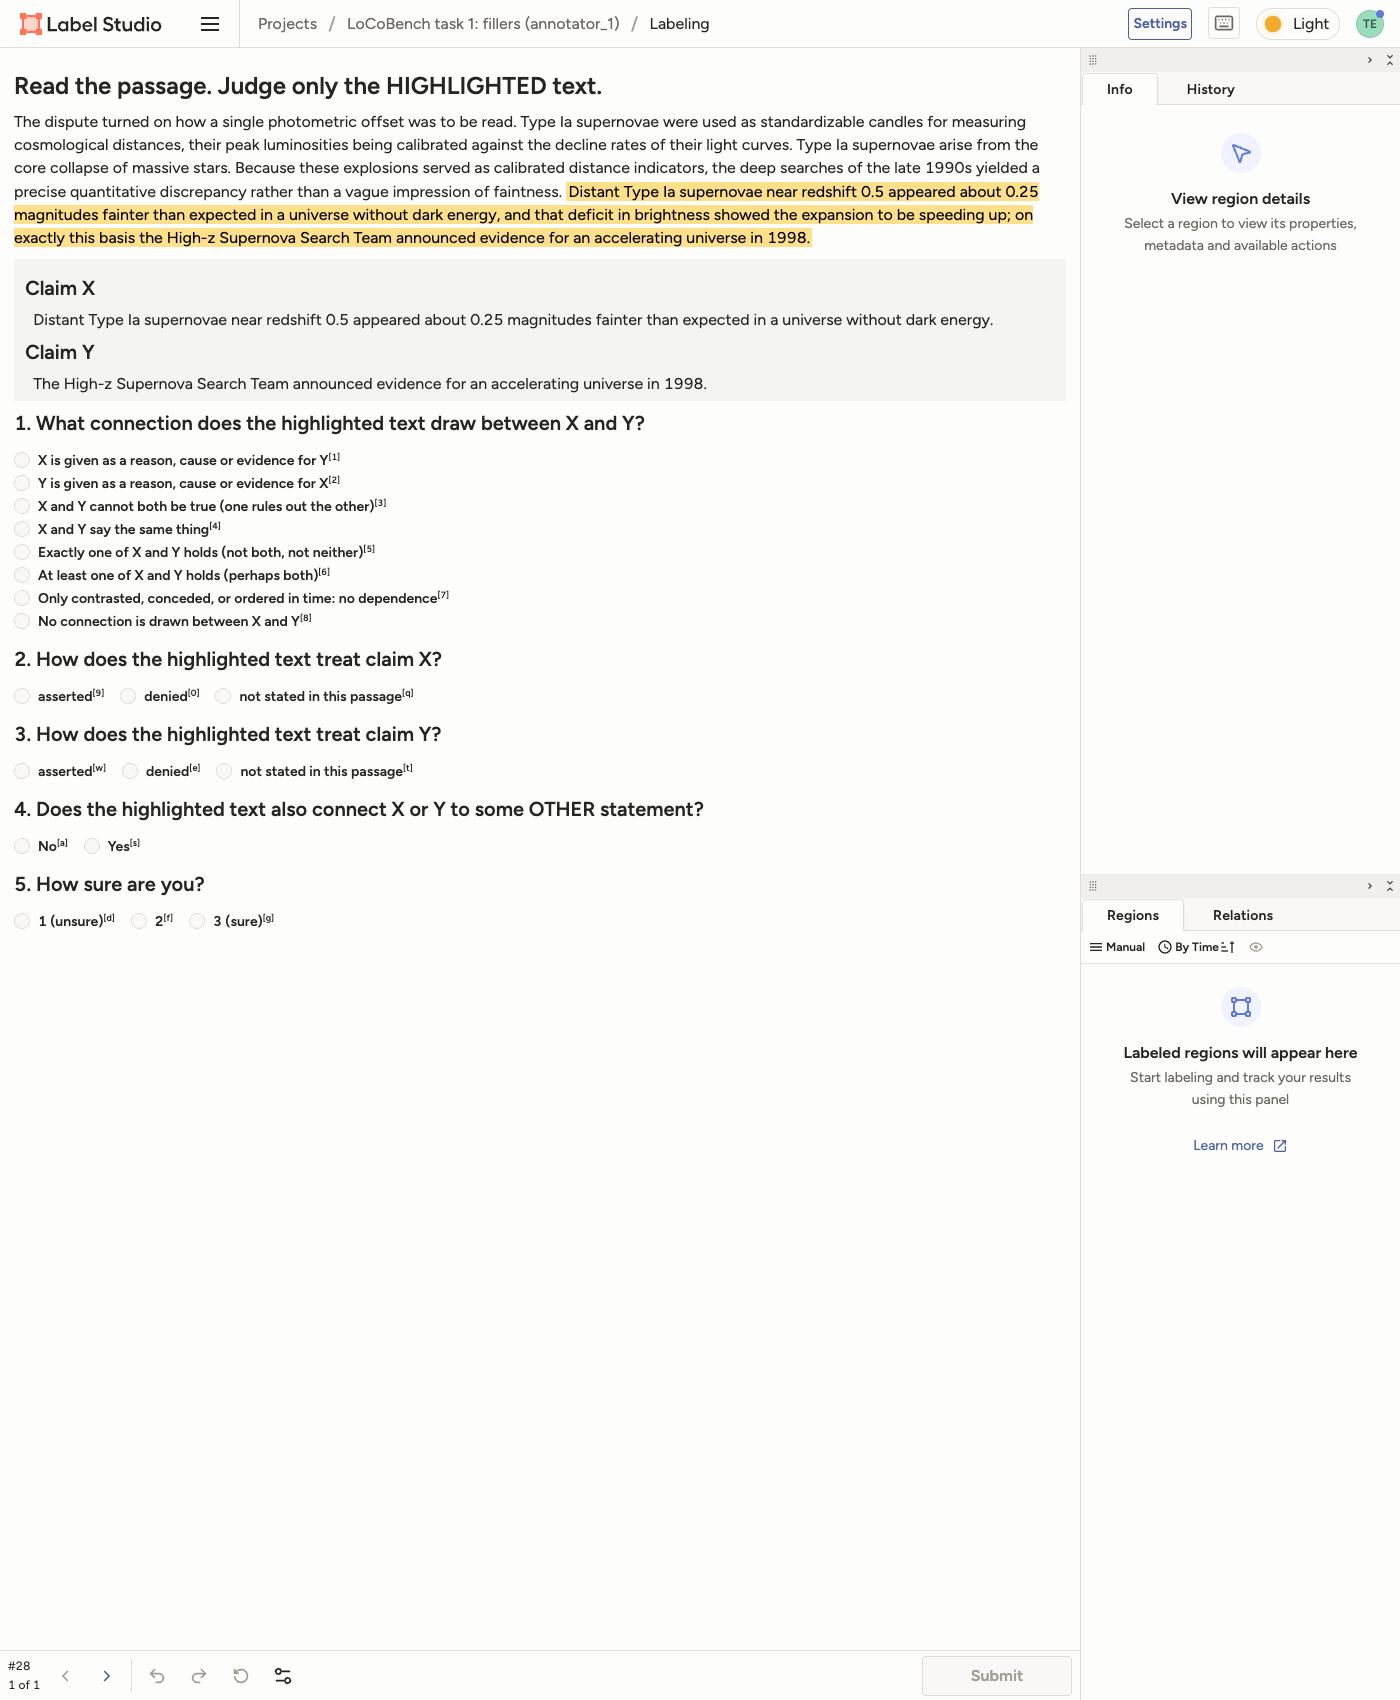
\includegraphics[width=0.9\textwidth,trim=0 755 325 45,clip]{figures/study_task1.png}}
\caption{\textbf{Task 1 in Label Studio}, as each annotator sees it locally: a filler
highlighted in its paragraph, the slot's two claims, and the five questions. Nothing on the screen
says which link was intended or whether the committee admitted the filler.}
\label{fig:study-ui}
\end{figure*}

\begin{figure*}[t]
\centering
\fbox{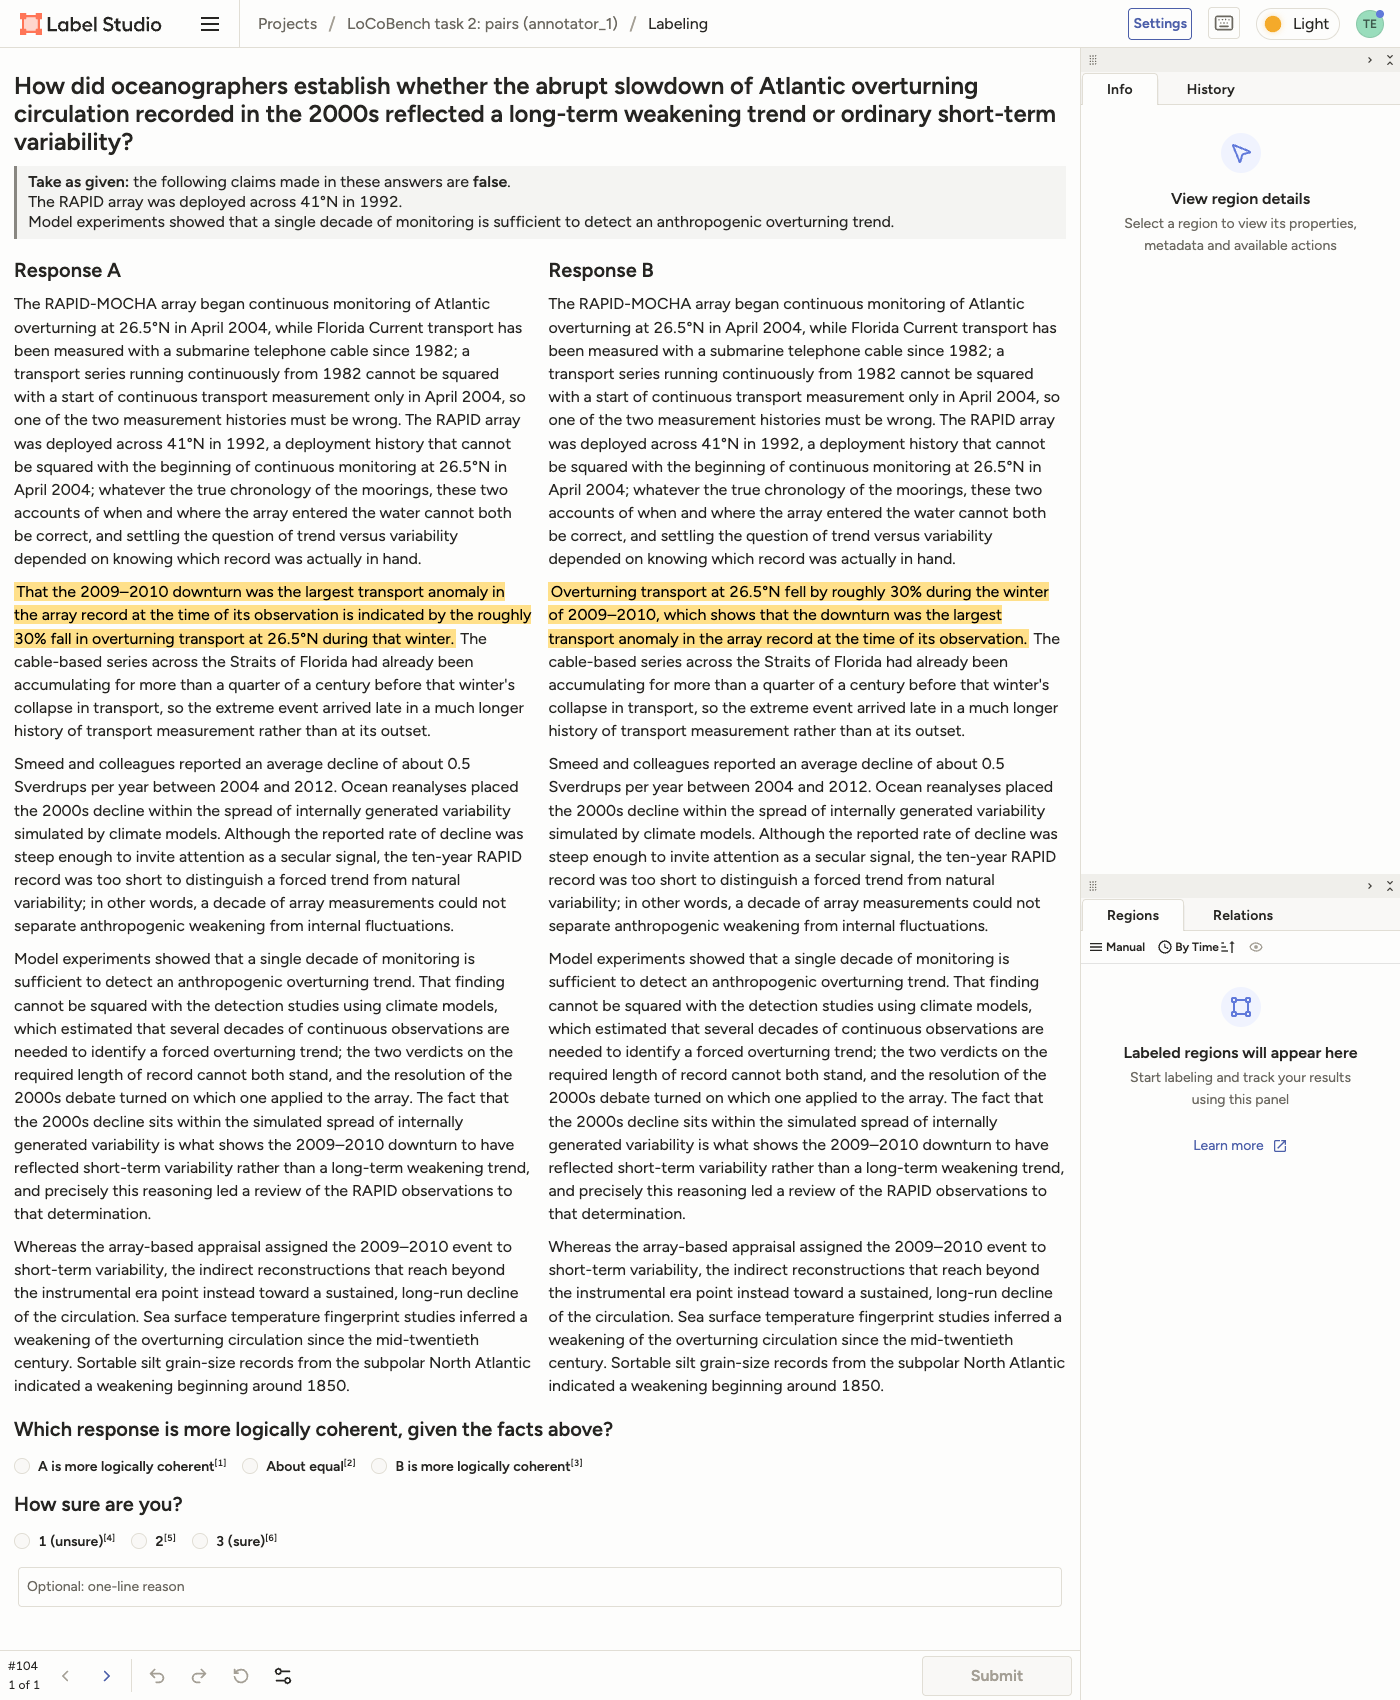
\includegraphics[width=0.9\textwidth,trim=0 520 325 45,clip]{figures/study_task2.png}}
\caption{\textbf{Task 2 in Label Studio} (top of the screen; the responses continue below, followed
by the preference, confidence and reason questions): the question, the family's false claims
given as facts, and two responses that differ only in the highlighted sentences.}
\label{fig:study-ui2}
\end{figure*}

Everything the study needs is generated by \texttt{scripts/locobench\_study\_build.py} from the
release and a fixed seed, and released with the paper:
\begin{itemize}[leftmargin=1.2em,itemsep=1pt,topsep=2pt]
\item one bundle per annotator, with its Task 1 and Task 2 files, the practice files, the two Label Studio labeling configurations, the annotator brief, setup
  instructions, the practice answers for the calibration discussion, and a script that creates
  the annotator's four projects in a local Label Studio;
\item the gold key, committed by hash in the pre-registration and never imported into Label
  Studio, which holds the sample, the intended answers, the committee's verdicts, the declared
  orders and the attention-check answers;
\item the pre-registration (hypotheses, sample, exclusions, scoring, power, consequences);
\item \texttt{scripts/locobench\_study\_analyze.py}, which checks the key against its hash,
  scores the Label Studio exports, and writes the report and the paper's macros. It was tested
  end to end on simulated exports, and on a real Label Studio instance (configuration validation,
  task import, annotation and JSON export), before annotation.
\end{itemize}

\paragraph{Task 1 options and their mapping.} The eight connection options map onto the
committee's SV5 labels: \emph{X is given as a reason, cause or evidence for Y} (and the reverse)
to the two directions of entailment; \emph{X and Y cannot both be true} to incompatibility;
\emph{say the same thing}, \emph{exactly one holds} and \emph{at least one holds} to equivalence,
exclusion and co-necessity; \emph{only contrasted, conceded, or ordered in time} and \emph{no
connection} to the no-factor readings, which score alike.

\paragraph{Budget.} Practice and calibration about 25 minutes, Task 1 about 75 minutes (72
fillers and 4 checks), Task 2 about two hours (18 families, 108 pairs and 2 checks), in sessions
of at most 90 minutes: 3.5--4 hours per annotator against a five-hour cap. \tbd{Measured times
and results.}


\end{document}
